\documentclass[11pt]{book}

\tolerance=600

% for \begin{center}, etc.
\usepackage[margin=1.0in]{geometry}

\usepackage{seqsplit}

% all kinds of math macros
\usepackage{amsmath}
\usepackage{amssymb}

% eps figures
\usepackage{epsfig}

% chapter title styles
\usepackage[Sonny]{fncychap}
\ChNameVar{\LARGE}
\ChTitleVar{\LARGE\sl}

% index
\usepackage{makeidx}
\makeindex


% part page style see
% http://tex.stackexchange.com/questions/6609/problems-with-part-labels-using-titlesec
\usepackage{titlesec}

\titleformat{\part}[display]
   {\Huge\filcenter}
   {{\partname{}} \thepart}
   {0em}
   {\hrule}



% hyperlinks -- load after fncychap
\usepackage{hyperref}

% color package
\usepackage[usenames]{color}

% longtable package used to split tables across pages
\usepackage{longtable}

% PDF-aware landscape package, used for rotating tables (including the
% longtable)
\usepackage{pdflscape}

% table coloring
\usepackage{colortbl}
\definecolor{tableShade}{rgb}{0.945,0.961,0.980}

% caption
\usepackage{caption}
\captionsetup[figure]{font=small,labelfont=small}

% make the MarginPars look pretty
\setlength{\marginparwidth}{0.75in}
\newcommand{\MarginPar}[1]{\marginpar{\vskip-\baselineskip\raggedright\tiny\sffamily
\hrule\smallskip{\color{red}#1}\par\smallskip\hrule}}

% to increase the likelihood that floats will occur "here" when you
% want them to
\renewcommand{\floatpagefraction}{1.0}
\renewcommand{\topfraction}{1.0}
\renewcommand{\bottomfraction}{1.0}
\renewcommand{\textfraction}{0.0}

% number subsubsections and put them in the TOC
\setcounter{tocdepth}{3}
\setcounter{secnumdepth}{3}

% custom hrule for title page
\newcommand{\HRule}{\rule{\linewidth}{0.125mm}}

% control sequences in verbatim
\usepackage{fancyvrb}

% short table of contents
\usepackage{shorttoc}

% spacing in the table of contents
\usepackage[titles]{tocloft}

\setlength{\cftbeforechapskip}{2ex}
\setlength{\cftbeforesecskip}{0.25ex}

% For splitting up lists into multitple columns
\usepackage{multicol}

% don't put a header on blank pages, see
% http://www.latex-community.org/forum/viewtopic.php?f=4&p=51559
% change ``plain'' to ``empty'' to eliminate the page number
\makeatletter
\renewcommand*\cleardoublepage{\clearpage\if@twoside
\ifodd\c@page\else
\hbox{}
\thispagestyle{empty}
\newpage
\if@twocolumn\hbox{}\newpage\fi\fi\fi}
\makeatother


% don't make the chapter/section headings uppercase.  See the fancyhdr
% documentation (section 9)
\usepackage{fancyhdr}
\renewcommand{\chaptermark}[1]{%
 \markboth{\chaptername
\ \thechapter.\ #1}{}}

\renewcommand{\sectionmark}[1]{\markright{\thesection---#1}}


% skip a bit of space between paragraphs, to enhance readability
\usepackage{parskip}



% special fraction
\newcommand{\sfrac}[2]{\mathchoice
  {\kern0em\raise.5ex\hbox{\the\scriptfont0 #1}\kern-.15em/
   \kern-.15em\lower.25ex\hbox{\the\scriptfont0 #2}}
  {\kern0em\raise.5ex\hbox{\the\scriptfont0 #1}\kern-.15em/
   \kern-.15em\lower.25ex\hbox{\the\scriptfont0 #2}}
  {\kern0em\raise.5ex\hbox{\the\scriptscriptfont0 #1}\kern-.2em/
   \kern-.15em\lower.25ex\hbox{\the\scriptscriptfont0 #2}}
  {#1\!/#2}}

\def\Ab {{\bf A}}
\def\eb {{\bf e}}
\def\Fb {{\bf F}}
\def\gb {{\bf g}}
\def\Hb {{\bf H}}
\def\ib {{\bf i}}
\def\Ib {{\bf I}}
\def\Kb {{\bf K}}
\def\lb {{\bf l}}
\def\Lb {{\bf L}}
\def\nb {{\bf n}}
\def\Pb {{\bf P}}
\def\Qb {{\bf Q}}
\def\rb {{\bf r}}
\def\Rb {{\bf R}}
\def\Sb {{\bf S}}
\def\ub {{\bf u}}
\def\Ub {{\bf U}}
\def\xb {{\bf x}}

\def\dt       {\Delta t}
\def\omegadot {\dot\omega}

\def\inp  {{\rm in}}
\def\outp {{\rm out}}
\def\sync {{\rm sync}}

\def\half   {\frac{1}{2}}
\def\myhalf {\sfrac{1}{2}}
\def\nph    {{n+\myhalf}}

% Level Set Macros
\def\ADDNODE       {{\tt{\bf ADDNODE}}}
\def\ADVANCE       {{\tt{\bf ADVANCE}}}
\def\done          {{\tt{\bf done}}}
\def\EVAL          {{\tt{\bf EVAL}}}
\def\INITPHI       {{\tt{\bf INITPHI}}}
\def\FASTMARCH     {{\tt{\bf FASTMARCH}}}
\def\FINDINTRFCE   {{\tt{\bf FINDINTRFCE}}}
\def\heap          {{\tt{\bf heap}}}
\def\heaploc       {{\tt{\bf heaploc}}}
\def\intface       {{\tt{\bf intface}}}
\def\intfacen      {{\tt{\bf intfacen}}}
\def\intfacenum    {{\tt{\bf intfacenum}}}
\def\intfacenumn   {{\tt{\bf intfacenumn}}}
\def\intfacenump   {{\tt{\bf intfacenump}}}
\def\intfacep      {{\tt{\bf intfacep}}}
\def\isnew         {{\tt{\bf isnew}}}
\def\LARGEINT      {{\tt{\bf LARGEINT}}}
\def\lvlerr        {{\tt{\bf lvlerr}}}
\def\LSCFL         {{\tt{\bf LSCFL}}}
\def\LStype        {{\tt{\bf LStype}}}
\def\LSnband       {{\tt{\bf LSnband}}}
\def\LSmine        {{\tt{\bf LSmine}}}
\def\mine          {{\tt{\bf mine}}}
\def\MINE          {{\tt{\bf MINE}}}
\def\mineloc       {{\tt{\bf mineloc}}}
\def\NARROWBAND    {{\tt{\bf NARROWBAND}}}
\def\nband         {{\tt{\bf nband}}}
\def\nbandnum      {{\tt{\bf nbandnum}}}
\def\nbandwidth    {{\tt{\bf nbandwidth}}}
\def\numtent       {{\tt{\bf numtent}}}
\def\PHIUPD        {{\tt{\bf PHIUPD}}}
\def\REINIT        {{\tt{\bf REINIT}}}
\def\RETYPIFY      {{\tt{\bf RETYPIFY}}}
\def\RMVNODE       {{\tt{\bf RMVNODE}}}
\def\sign          {{\tt{\bf sign}}}
\def\type          {{\tt{\bf type}}}
\def\UPDATE        {{\tt{\bf UPDATE}}}
\def\UPDATEF       {{\tt{\bf UPDATEF}}}
\def\UPDATENODE    {{\tt{\bf UPDATENODE}}}
\def\new           {{\rm new}}
\def\old           {{\rm old}}


\usepackage{listings}

\usepackage{subfig}

\definecolor{gray}{rgb}       {0.8,0.8,0.8}
\definecolor{light-blue}{rgb} {0.8,0.8,1.0}
\definecolor{light-green}{rgb}{0.8,1.0,0.8}
\definecolor{light-red}{rgb}  {1.0,0.9,0.9}

\lstset{frame=single,basicstyle=\footnotesize\ttfamily,showstringspaces=false,showspaces=false,xleftmargin=5pt,xrightmargin=6pt}

\lstset{language=C++,
                basicstyle=\footnotesize\ttfamily,
                keywordstyle=\color{blue}\footnotesize\ttfamily,
                commentstyle=\color{cyan}\footnotesize\ttfamily
}

\lstdefinelanguage{cpp}{
  language     = C++,
  morekeywords =
  [2]{amrex,amrex_real,
      Array,BaseFab,Box,BoxArray,DistributionMapping,FabArray,FArrayBox,
      Geometry,IArrayBox,IntVect,IndexType,MFIter,MultiFab,
      ParallelDescriptor,ParmParse,Real,RealBox,
      AMREX_SPACEDIM,AMREX_D_DECL},
  keywordstyle = [2]\color{red}\footnotesize\ttfamily,
}

% \lstset{
%   basicstyle=\small\ttfamily,%
%   frame=single,%
%   rulesepcolor=\color{gray},%
%   backgroundcolor=\color{white}%
% }
% \lstset{belowskip=-0.25em}


% Macros for indexing
\newcommand{\idxamrex}[1]{\index{\tt{amrex}!{\tt #1}}{\tt #1}}

%------------------------------------------------------------------------------
\input amrexsymbols
% \graphicspath{{Verification/}{Software/}{ConvertCheckpoint/}{Scaling/}{Visualization/}}


%------------------------------------------------------------------------------
\begin{document}



\frontmatter

\begin{titlepage}
\begin{center}
\ \\[3in]
{\sf \Huge AMReX}
\ \\[0.2in]

\begin{minipage}{5.5in}
\HRule\\[2mm]
\centering
{\Large \em An adaptive mesh refinement software framework}

\HRule
\end{minipage}

\ \\[.5 in]
{\sf \huge User's Guide}

\vfill

{\large AMReX Developers}
\ \\[0.3 in]
{\large \today}
\end{center}

\end{titlepage}


\shorttoc{Chapter Listing}{0}

\setcounter{tocdepth}{2}
\tableofcontents

\clearpage

\listoffigures
\addcontentsline{toc}{chapter}{list of figures}

\clearpage

\listoftables
\addcontentsline{toc}{chapter}{list of tables}


\cleardoublepage

\chapter*{Preface}
\addcontentsline{toc}{chapter}{Preface}
\noindent The current version of the \BoxLib\ User's Guide can be found in 
the \BoxLib\ git repository in {\tt BoxLib/docs}.  Visit our website
at {\tt https://ccse.lbl.gov} for free access to \BoxLib.  Any questions,
comments, suggestions, etc., regarding this User's Guide should be directed
to Andy Nonaka of CCSE at {\tt AJNonaka@lbl.gov}.  Further information 
about \BoxLib\ can be found by contacting Ann Almgren of CCSE at 
{\tt ASAlmgren@lbl.gov} or by visiting our website.\\

\noindent (c) 1996-2000 The Regents of the University of California (through
E.O. Lawrence Berkeley National Laboratory), subject to approval by
the U.S. Department of Energy.  Your use of this software is under
license -- the license agreement is attached and included in the
\BoxLib\ home directory as license.txt or you may contact Berkeley Lab's Technology
Transfer Department at TTD@lbl.gov.  NOTICE OF U.S. GOVERNMENT RIGHTS.
The Software was developed under funding from the U.S. Government
which consequently retains certain rights as follows: the
U.S. Government has been granted for itself and others acting on its
behalf a paid-up, nonexclusive, irrevocable, worldwide license in the
Software to reproduce, prepare derivative works, and perform publicly
and display publicly.  Beginning five (5) years after the date
permission to assert copyright is obtained from the U.S. Department of
Energy, and subject to any subsequent five (5) year renewals, the
U.S. Government is granted for itself and others acting on its behalf
a paid-up, nonexclusive, irrevocable, worldwide license in the
Software to reproduce, prepare derivative works, distribute copies to
the public, perform publicly and display publicly, and to permit
others to do so.\\



\mainmatter

\chapter{Introduction}\label{Chap:Introduction}
\amrex\ is a publicly available software framework designed for
building massively parallel block-structured adaptive mesh refinement
(AMR) applications.

Key features of \amrex\ include:
\begin{itemize}
\item \cpp\ and Fortran interfaces
\item 1-, 2- and 3-D support
\item Support for cell-centered, face-centered, edge-centered, and
  nodal data
\item Support for hyperbolic, parabolic, and elliptic solves on
  hierarchical adaptive grid structure
\item Optional subcycling in time for time-dependent PDEs
\item Support for particles
\item Parallelization via flat MPI, OpenMP, hybrid MPI/OpenMP, or MPI/MPI
\item Parallel I/O
\item Plotfile format supported by \amrvis, \visit, \paraview, and \yt.
\end{itemize}

Because \amrex's core is mainly written in \cpp, the basics of \amrex\
is first introduced in \cpp\ and then their Fortran wrappers if
available will be described as well.  

Besides the User's Guide, there is document generated by Doxygen at
\url{https://ccse.lbl.gov/pub/AMReX_Docs/}.  Documentation on
migration from \boxlib\ is available at {\tt Docs/Migration}.


\chapter{Getting Started}\label{Chap:GettingStarted}
We now proceed through a series of tutorial applications of increasing complexity
to help understand how to write your own application.  Any of these examples
can be used as a starting point for your own application.  Each of the examples
will be presented in Fortran90 and C++.  The examples are contained in the \BoxLib\
release found at {\tt https://ccse.lbl.gov/pub/BoxLib/}.

\section{Diffusion Equation - Fortran90}
Our first example, contained in {\tt BoxLib/Tutorials/WaveEquation\_F/}, advances the 
equations
\begin{eqnarray}
\frac{\partial\phi_1}{\partial t} &=& \phi_2, \\
\frac{\partial\phi_2}{\partial t} &=& \nabla^2\phi_1,
\end{eqnarray}
on a domain from -1 to 1 in each spatial direction with initial conditions
\begin{eqnarray}
\phi_1(t=0) &=& 0 \\
\phi_2(t=0) &=& e^{-100r^2},
\end{eqnarray}
where $r$ is the distance from the cell-center to the center of the domain.
We use uniform grid spacing in each direction, i.e., $\Delta x = \Delta y = \Delta z$,
and for this example, we used a fixed time step with $\Delta t = 0.1\Delta x$.
To advance these equations, we use a Runge-Kutta temporal discretization and a 
fourth-order spatial discretization of the Laplacian.  This example does not use AMR, 
and uses periodic boundary conditions on all sides.

In the problem directory, you will see the following files:
\begin{itemize}
\item {\tt GNUmakefile}

This contains compiler settings and directories required by the make system to build the code.

  \begin{itemize}

    \item {\tt BOXLIB\_HOME}

    Change this to point to the \BoxLib\ home directory.  Alternatively, you can define {\tt BOXLIB\_HOME}
    as an environment variables on your system.

    \item {\tt MKVERBOSE}

    Verbosity of compile-time output.

    \item {\tt NDEBUG}
      
    ``Not Debug'' (we know, confusing).  If 't', modifies compiler flags to build a more optimized version
    of the code.

    \item {\tt MPI}

    Indicate whether you want your executable to be MPI-compatible.  In general there is no reason to turn this
    off since you can still run the resulting executable serially.

    \item {\tt OMP}

    Turns on OpenMP compiler flags.  Note that you still must write OpenMP directives into your code.

    \item {\tt COMP}

    The compiler.  Supported options include Intel, PathScale, and PGI.  gfortran seems to be bug-free
    on all systems we've run on.  Intel after version 9 seems flaky.  PathScale (available at OLCF and NERSC)
    seems to work as long as you don't turn the optimization flags too high.  PGI seems to work fine, but
    is slower than the others.

  \end{itemize}

\item {\tt GPackage.mak}

List of local files needed to be included in the build.  The {\tt GNUmakefile} points to this.

\item {\tt main.f90}, {\tt init\_data.f90}, {\tt advance.f90}, {\tt write\_plotfile.f90}

Source code that is not within the {\tt BoxLib/Src/} tree.  Note: if a file that exists in the
{\tt BoxLib/Src/} tree also exists in the local directory, the local copy takes precedence.
{\tt main.f90} is the driver program that calls subroutines from the other Fortran90 files.

\item {\tt inputs\_2d}, {\tt inputs\_3d}

Inputs files to customize the simulation parameters.

\end{itemize}

To build the code, simply type ``make''.  An exectubale will appear that has some indication (but not complete)
about what setting you used in the {\tt GNUmakefile}.  To run the code serially, simply type, for example,
\begin{verbatim}
./main.Linux.gfortran.mpi.exe inputs_2d
\end{verbatim}
To run in parallel, if you have MPI on your machine, instead type, for example,
\begin{verbatim}
mpiexec -n 4 ./main.Linux.gfortran.mpi.exe inputs_2d
\end{verbatim}
In the parallel case,you should see the following on your screen at the beginning
\begin{verbatim}
MPI initialized with            4  MPI processes
MPI initialized with            1  threads
\end{verbatim}
The program will complete and there will be a series of plotfiles, e.g., {\tt plt00000}, in the run directory.
You can open these using {\tt VisIt} (available at {\tt https://wci.llnl.gov/codes/visit/}) by opening
the {\tt Header} file within the plotfile directory.  (For the {\tt VisIt} novice, after you open the {\tt Header}
file, select ``Add'' $\rightarrow$ ``Pseudocolor'' $\rightarrow$ ``Variable 2'' and then click ``Draw''.)


\chapter{Building AMReX}\label{Chap:BuildingAMReX}

In this chapter, we discuss \amrex's build systems.  There are three
ways to use \amrex.  The approach used by \amrex\ developers uses GNU
Make.  There is no installation step in this approach.  Application
codes adopt \amrex's build system and compile \amrex\ while compiling
their own codes.  This will be discussed in more details in
Section~\ref{sec:build:make}.  The second approach is to build \amrex\
into a library and install it (Section~\ref{sec:build:lib}).  Then an
application code uses its own build system and links \amrex\ as an
external library.  \amrex\ can also be built with CMake
(Section~\ref{sec:build:cmake}).

\section{Building with GNU Make}
\label{sec:build:make}

In this build approach, you write your own make files defining a
number of variables and rules.  Then you invoke {\tt make} to start
the building process.  This will result in an executable upon
successful completion.  The temporary files generated in the building
process are stored in a temporary directory named {\tt
  tmp\_build\_dir}.

\subsection{Dissecting a Simple Make File}

An example of building with GNU Make can be found in {\tt
  amrex/Tutorials/Basic/HelloWorld\_C}.  Table~\ref{tab:makevarimp}
shows a list of important variables.
\begin{table}[t]
  \centering
  \begin{tabular}{lcc}
    Variable & Value & Default \\
    \hline
    {\tt AMREX\_HOME} & Path to amrex & environment \\
    {\tt COMP} & {\tt gnu}, {\tt cray}, {\tt intel}, {\tt llvm}, or {\tt pgi} & none \\
    {\tt DEBUG} & {\tt TRUE} or {\tt FALSE} & {\tt TRUE} \\
    {\tt DIM} & 1 or 2 or 3 & none \\
    {\tt USE\_MPI} & {\tt TRUE} or {\tt FALSE} & {\tt FALSE} \\
    {\tt USE\_OMP} & {\tt TRUE} or {\tt FALSE} & {\tt FALSE} \\
    \hline
  \end{tabular}
  \caption{\label{tab:makevarimp} Important make variables}
\end{table}

At the beginning of {\tt
  amrex/Tutorials/Basic/HelloWorld\_C/GNUmakefile}, {\tt AMREX\_HOME}
is set to the path to the top directory of \amrex.  Note that in the
example {\tt ?=} is a conditional variable assignment operator that
only has an effect if {\tt AMREX\_HOME} has not been defined
(including in the environment).  One can also set it through
environment variable.  For example in bash, one can set {\tt export
  AMREX\_HOME=/path/to/amrex}.

One must set the {\tt COMP} variable to choose a compiler.  Currently
the list of supported compilers includes {\tt gnu}, {\tt cray}, {\tt
  intel}, {\tt llvm}, and {\tt pgi}.  One must also set the {\tt DIM}
variable to either 1, 2, or 3, depending on the dimensionality of the
problem. 

Variables {\tt DEBUG}, {\tt USE\_MPI} and {\tt USE\_OMP} are optional
with default set to {\tt TRUE}, {\tt FALSE} and {\tt FALSE},
respectively.  The meaning of these variables should be obvious.  In
{\tt DEBUG} build, aggressive compiler optimization flags are turned
off and assertions in \amrex\ source code are turned on.  For
production runs, {\tt DEBUG} should be set to {\tt FALSE}.

After defining these make variables, a number of files, {\tt
  Make.defs}, {\tt Make.package} and {\tt Make.rules}, are included in
{\tt GNUmakefile}.  \amrex\ are split into a number of packages.  An
application code does not include every package.  In this simple
example, we only need to include {\tt
  \$(AMREX\_HOME)/Src/Base/Make.package}.  An application code also
has its own {\tt Make.package} file (e.g., {\tt ./Make.package} in
this example) to append source files to the build system using
operator {\tt +=}.  Variables for various source files are shown
below.
\begin{quote}
\begin{description}
\item [{CEXE\_sources}] \cpp\ source files.  Note that \cpp\
  source files are assumed to have a {\tt .cpp} extension.
\item [{CEXE\_headers}] \cpp\ headers with {\tt .h} or {\tt .H} extension.
\item [{cEXE\_sources}] C source files with {\tt .c} extension.
\item [{cEXE\_headers}] C headers with {\tt .h} extension.
\item [{f90EXE\_sources}] Free format Fortran source with {\tt
    .f90} extension.
\item [{F90EXE\_sources}] Free format Fortran source with {\tt
    .F90} extension.  Note that these Fortran files will go through
  preprocessing.
\end{description}
\end{quote}
In this simple example, the extra source file, {\tt main.cpp} is in
the current directory that is already in the build system's search
path.  If this example has files in a subdirectory (e.g., {\tt
  mysrcdir}), you will then need to add the following to {\tt
  Make.package}. 
\begin{verbatim}
    VPATH_LOCATIONS += mysrcdir
    INCLUDE_LOCATIONS += mysrcdir
\end{verbatim}
Here {\tt VPATH\_LOCATIONS} and {\tt INCLUDE\_LOCATIONS} are the search
path for source and header files, respectively.

\subsection{Tweaking Make System}

The GNU Make build system is located at {\tt amrex/Tools/GNUMake}.
You can read {\tt README.md} and the make files there for more
information.  Here we will give a brief overview.

Besides building executable, other common make commands include:
\begin{quote}
\begin{description}
  \item[make clean] This removes the executable, {\tt .o} files, and
    the temporarily generated files.  Note that one can add additional
    targets to this rule by using the double colon (::)
  \item[make realclean] This removes all files generated by make.
  \item[make help] This shows the rules for compilation.
  \item[make print-xxx] shows the value of varible {\tt xxx}.  This is
    very useful for debugging and tweaking the make system.
\end{description}
\end{quote}

Compiler flags are set in {\tt amrex/Tools/GNUMake/comps/}.  Note that
variables like {\tt CC} and {\tt CFLAGS} are reset in that directory
and their values in environment variables are disregarded. Site
specific setups (e.g., MPI installation) are in {\tt
  amrex/Tools/GNUMake/sites/}, which includes a generic setup in {\tt
  Make.unknown}.  You can override the setup by having your own {\tt
  Make.\$(host\_name)} file, where variable {\tt host\_name} is your
host name in the make system and can be found via {\tt make
  print-host\_name}.  You can also have a {\tt
  amrex/Tools/GNUMake/Make.local} file to override various variables.
See {\tt amrex/Tools/GNUMake/Make.local.template} for an example.

\section{Building {\tt libamrex}}
\label{sec:build:lib}

If an application code already has its own elaborated build system and
wants to use \amrex\ as an external library, this might be your
choice.  In this approach, one runs {\tt ./configure}, followed by
{\tt make} and {\tt make install}.  In the top \amrex\ directory, one
can run {\tt ./configure -h} to show the various options for the {\tt
  configure} script.  This approach is built on the \amrex\ GNU Make
system.  Thus Section~\ref{sec:build:make} is recommended if any fine
tuning is needed.

\section{Building with CMake}
\label{sec:build:cmake}

\MarginPar{todo}



\chapter{{\tt Base} Source Code}\label{Chap:Basics}
In this chapter, we present the basics of \amrex.  The implementation
source codes are in {\tt amrex/Src/Base/}.  Note that \amrex\ classes
and functions are in namespace {\tt amrex}.  For clarity, we usually
drop {\tt amrex::} in the example codes here.  It is also assumed that
headers have been properly {\tt include}d.  We recommend you study
tutorials at {\tt amrex/Tutorials/Basic/} while reading this chapter.
After reading this chapter, one should be able to develop single-level
parallel codes using \amrex.  It should also be noted that this is not
a comprehensive reference manual.

\section{Dimensionality}
\label{sec:basics:dim}

As we have mentioned in Chapter~\ref{Chap:BuildingAMReX}, the
dimensionality of \amrex\ must be set at compile time.  A macro, {\tt
  AMREX\_SPACEDIM}, is defined to be the number of spatial
dimensions.  C++ codes can also use the {\tt amrex::SpaceDim}
variable.  Fortran codes can use either the macro and preprocessing or
do 
\begin{verbatim}
    use amrex_fort_module, only : amrex_spacedim
\end{verbatim}
The coordinate directions are zero based. \MarginPar{Not in Fortran}

\section{Array}

{\tt Array} class is derived from {\tt std::vector}.  The only
difference between {\tt Array} and {\tt std::vector} is that {\tt
  Array::operator[]} provides bound checking when compiled with {\tt
  DEBUG=TRUE}. 

\section{Real}

\amrex\ can be compiled to use either double precision (which is the
default) or single precision.  {\tt amrex::Real} is {\tt typedef}'d to
either {\tt double} or {\tt float}.  C codes can use {\tt
  amrex\_real}.  The data type is accessible in Fortran codes via
\begin{verbatim}
    use amrex_fort_module, only : amrex_real
\end{verbatim}

\section{ParallelDescriptor}

\amrex\ users do not need to use MPI directly.  Parallel communication
is often handled by the data abstraction classes (e.g., {\tt
  MultiFab}; Section~\ref{sec:basics:multifab}).  In addition, \amrex\
has provided {\tt namespace ParallelDesriptor}.  The frequently used
functions are 
\begin{lstlisting}[language=cpp]
 int myproc = ParallelDescriptor::MyProc();  // Return the rank
 
 int nprocs = ParallelDescriptor::NProcs();  // Return the number of processes
 
 if (ParallelDescriptor::IOProcessor()) { 
     // Only the I/O process executes this
 }
 
 int ioproc = ParallelDescriptor::IOProcessorNumber();  // I/O rank
 
 ParallelDescriptor::Barrier();
 
 // Broadcast 100 ints from the I/O Processor
 Array<int> a(100);
 ParallelDescriptor::Bcast(a.data(), a.size(),
                     ParallelDescriptor::IOProcessorNumber())
 
 // See AMReX_ParallelDescriptor.H for many other Reduce functions 
 ParallelDescriptor::ReduceRealSum(x);
\end{lstlisting}

\section{Print}
\label{sec:basics:print}

\amrex\ provides classes for printing messages to standard output or
any \cpp\ {\tt ostream}.  The main reason one should use them instead
of {\tt std::cout} is that messages from multiple processes or
threads do not get mixed up.  Below are some examples.
\begin{lstlisting}[language=cpp]
 Print() <<  "x = " << x << "\n"; // Print on I/O processor
 
 Real pi = std::atan(1.0)*4.0;
 // Print on rank 3 with precision of 17 digits
 // SetPrecision does not modify cout's floating-point decimal precision setting.
 Print(3).SetPrecision(17) << pi << "\n";

 int oldprec = std::cout.precision(10);
 Print() << pi << "\n";  // Print with 10 digits
 
 AllPrint() << "Every process prints\n";  // Print on every process
 
 std::ofstream ofs("my.txt", std::ofstream::out);
 Print(ofs) << "Print to a file" << std::endl;
 ofs.close();
\end{lstlisting}

\section{ParmParse}

{\tt ParmParse} is a class providing a database for the storage and
retrieval of command-line and input-file arguments.  When {\tt
  amrex::Initialize()} is called, the first command-line argument
after the executable name (if there is one and it does not contain
character {\tt =}) is taken to be the inputs file, and the contents in
the file are used to initialized the {\tt ParmParse} database.  The
rest of the command-line arguments are also parsed by {\tt ParmParse}.
The format of the inputs file is a series of definitions in the form
of {\tt prefix.name = value value ...}.  For each line, texts after a
{\tt \#} are comments.  Here is an example inputs file.
\begin{verbatim}
nsteps    = 100               # integer
nsteps    = 1000              # nsteps appears a second time
dt        = 0.03              # floating point number
ncells    = 128 64 32         # a list of 3 ints
xrange    = -0.5 0.5          # a list of 2 reals
title     = "Three Kingdoms"  # a string
hydro.cfl = 0.8               # with prefix, hydro 
\end{verbatim}
The following code shows how to use {\tt ParmParse} to get the values.
\begin{lstlisting}[language=cpp]
 ParmParse pp;
 
 int nsteps = 0;
 pp.query("nsteps", nsteps);
 amrex::Print() << nsteps << "\n";  // 1000
 
 Real dt;
 pp.get("dt", dt);  // runtime error if dt is not in inputs
 
 Array<int> numcells;
 // A different name say 'numcells' can be used
 pp.getarr("ncells", numcells);
 amrex::Print() << numcells.size() << "\n";  // 3
 
 Array<Real> xr {-1.0, 1.0};
 if (!queryarr("xrange", xr)) {
     amrex::Print() << "Cannot find xrange in inputs, "
                    << "so the default {-1.0,1.0} will be used\n";
 }
 
 std::string title;
 query("title", title);  // query string
 
 ParmParse pph("hydro");  // with prefix 'hydro'
 Real cfl;
 pph.get("cfl", cfl);    // get parameter with prefix
\end{lstlisting}
Note that when there are multiple definitions for a parameter {\tt
  ParamParse} by default returns the last one.  The difference between
{\tt query} and {\tt get} should also be noted.  It is a runtime error
if {\tt get} fails to get the value, whereas {\tt query} returns an
error code without generating a runtime error that will abort the run.
If it is sometimes convenient to override parameters with command-line
arguments without modifying the inputs file.  The command-line
arguments after the inputs file are added later to the database and
are therefore used be default.  For example, one can run with
\begin{verbatim}
    myexecutable myinputsfile ncells="64 32 16" hydro.cfl=0.9
\end{verbatim}
to change the value of {\tt ncells} and {\tt hydro.cfl}.

\section{Box, IntVect and IndexType}
\label{sec:basics:box}

In \amrex, the computational domain (on each AMR level) is decomposed
into a union of rectangular domains.  {\tt Box} is the data
structure for representing such rectangular domains in indexing space.
{\tt Box} is a dimension dependent class.  It has lower and upper
corners (represented by {\tt IntVect} and an index type
(represented by {\tt IndexType}).  There are no floating-point data in
the object.

\subsection{IntVect}

{\idxamrex{IntVect}} is a dimension dependent class representing an
integer vector in {\idxamrex{AMREX\_SPACEDIM}}-dimensional space.  An
{\tt IntVect} can be constructed as follows,
\begin{lstlisting}[language=cpp]
 IntVect iv(AMREX_D_DECL(19, 0, 5));
\end{lstlisting}
Here {\tt AMREX\_D\_DECL} is a macro that expands {\tt
  AMREX\_D\_DECL(19,0,5)} to either {\tt 19} or {\tt 19,0} or {\tt
  19,0,5} depending on the number of dimensions.  The data can be
accessed via {\tt operator[]}, and the internal data pointer can be
returned by function {\tt getVect}.  For example
\begin{lstlisting}[language=cpp]
 for (int idim = 0; idim < AMREX_SPACEDIM; ++idim) {
     amrex::Print() << "iv[" << idim << "] = " << iv[idim] << "\n";
 }
 const int * p = iv.getVect();  // This can be passed to Fortran/C as an array
\end{lstlisting}

The class has a static function {\tt TheZeroVector()} returning the
zero vector, {\tt TheUnitVector()} returning the unit vector, and {\tt
  TheDimensionVector (int dir)} returning a reference to a constant
{\tt IntVect} that is zero except in the {\tt dir}-direction.  Note
the direction is zero-based.  {\tt IntVect} has a number of relational
operators, {\tt ==}, {\tt !=}, {\tt <}, {\tt <=}, {\tt >}, and {\tt
  >=} that can be used for lexicographical comparison (e.g., key of
{\tt std::map}), and a class {\tt IntVect::shift\_hasher} that can be
used as a hash function (e.g., for {\tt std::unordered\_map}).  It
also has various arithmetic operators.  For example,
\begin{lstlisting}[language=cpp]
 IntVect iv(AMREX_D_DECL(19, 0, 5));
 IntVect iv2((AMREX_D_DECL(4, 8, 0));
 iv += iv2;  // iv is now (23,8,5)
 iv *= 2;    // iv is now (46,16,10);
\end{lstlisting}

In AMR codes, one often needs to do refinement and coarsening on {\tt
  IntVect}.  The refinement operation can be done with the
multiplication operation.  However, the coarsening requires care
because of the rounding towards zero behavior of integer division in
Fortran, C and C++.  For example {\tt int i = -1/2} gives {\tt i =
  0}, and what we want is usually {\tt i = -1}.  Thus, one should use
the {\tt coarsen} functions:
\begin{lstlisting}[language=cpp]
  IntVect iv(AMREX_D_DECL(127,127,127));
  IntVect coarsening_ratio(AMREX_D_DECL(2,2,2));
  iv.coarsen(2);                 // Coarsen each component by 2
  iv.coarsen(coarsening_ratio);  // Component-wise coarsening
  const auto& iv2 = amrex::coarsen(iv, 2); // Return an IntVect w/o modifying iv
  IntVect iv3 = amrex::coarsen(iv, coarsening_return); // iv not modified
\end{lstlisting}

Finally, we note that {\tt operator<<} is overloaded for {\tt
  IntVect} and therefore one can call
\begin{lstlisting}[language=cpp]
  amrex::Print() << iv << "\n";
  std::cout << iv << "\n";
\end{lstlisting}

\subsection{IndexType}

This class defines an index as being cell based or node based in
each dimension.  The default constructor defines a cell based type in
all directions.  One can also construct an {\tt IndexType} with an
{\tt IntVect} with zero and one representing cell and node,
respectively.
\begin{lstlisting}[language=cpp]
 // Node in x-direction and cell based in y and z-directions
 // (i.e., x-face of numerical cells)
 IndexType xface(IntVect{AMREX_D_DECL(1,0,0)});
\end{lstlisting}
The class provides various functions including
\begin{lstlisting}[language=cpp]
 // True if the IndexType is cell based in all directions.
 bool cellCentered () const;

 // True if the IndexType is cell based in dir-direction.
 bool cellCentered (int dir) const;

 // True if the IndexType is node based in all directions.
 bool nodeCentered () const;

 // True if the IndexType is node based in dir-direction.
 bool nodeCentered (int dir) const;
\end{lstlisting}

Index type is a very important concept in \amrex.  It is a way of
representing the notion of indices $i$ and $i+1/2$.  

\subsection{Box}

A {\tt Box} is an abstraction for defining discrete regions of {\tt
  AMREX\_SPACEDIM}-dimensional indexing space.  {\tt Box}es have an
{\tt IndexType} and two {\tt IntVect}s representing the lower and
upper corners.  Boxes can exist in positive and negative indexing
space.   Typical ways of defining a {\tt Box} are
\begin{lstlisting}[language=cpp]
 IntVect lo(AMREX_D_DECL(64,64,64));
 IntVect hi(AMREX_D_DECL(127,127,127));
 IndexType typ({AMREX_D_DECL(1,1,1)});
 Box cc(lo,hi);        // By default, Box is cell based.
 Box nd(lo,hi+1,typ);  // Construct a nodal Box.
 Print() << "A cell-centered Box " << cc << "\n";
 Print() << "An all nodal Box    " << nd << "\n";
\end{lstlisting}
Depending the dimensionality, the output of the code above is
\begin{verbatim}
  A cell-centered Box ((64,64,64) (127,127,127) (0,0,0))
  An all nodal Box    ((64,64,64) (128,128,128) (1,1,1))
\end{verbatim}
For simplicity, we will assume it is 3D for the rest of this section.
In the output, three integer tuples for each box are the lower corner
indices, upper corner indices, and the index types.  Note that {\tt 0}
and {\tt 1} denote cell and node, respecitively.  For each tuple like
{\tt (64,64,64)}, the 3 numbers are for 3 directions.  The two {\tt
  Box}es in the code above represent different indexing views of the
same domain of $64^3$ cells.  Note that in \amrex\ convention, the
lower side of a cell has the same integer value as the cell centered
index.  That is if we consider a cell based index represent $i$, the
nodal index with the same integer value represents $i-1/2$.  

There are a number of ways of converting a {\tt Box} from one type to
another.
\begin{lstlisting}[language=cpp]
  Box b0 ({64,64,64}, {127,127}); // Index type: (cell, cell, cell)

  Box b1 = surroundingNodes(b0);  // A new Box with type (node, node, node)
  Print() << b1;                  // ((64,64,64) (128,128,128) (1,1,1))
  Print() << b0;                  // Still ((64,64,64) (127,127,127) (0,0,0))

  Box b2 = enclosedCells(b1);     // A new Box with type (node, node, node)
  if (b2 == b0) {                 // Yes, they are identical.
     Print() << "b0 and b2 are identical!\n";
  }

  Box b3 = convert(b0, {0,1,0});  // A new Box with type (cell, node, cell)
  Print() << b3;                  // ((64,64,64) (127,128,127) (0,1,0))

  b3.convert({0,0,1});            // Convert b0 to type (cell, cell, node)
  Print() << b3;                  // ((64,64,64) (127,127,128) (0,0,1))

  b3.surroundingNodes();          //  Exercise for you
  b3.enclosedCells();             //  Exercise for you
\end{lstlisting}

The internal data of {\tt Box} can be accessed via various member functions.
Examples are
\begin{lstlisting}[language=cpp]
  const IntVect& smallEnd () const&;  // Get the small end of the Box
  int bigEnd (int dir) const;         // Get the big end in dir direction
  const int* loVect () const&;        // Get a const pointer to the lower end
  const int* hiVect () const&;        // Get a const pointer to the upper end
\end{lstlisting}

{\tt Box}es can be refined and coarsened.  Refinement or coarsening
does not change the index type.  Some examples are shown below.
\begin{lstlisting}[language=cpp]
  Box ccbx ({16,16,16}, {31,31,31});
  ccbx.refine(2);
  Print() << ccbx;                   // ((32,32,32) (63,63,63) (0,0,0))
  Print() << ccbx.coarsen(2);        // ((16,16,16) (31,31,31) (0,0,0))

  Box ndbx ({16,16,16}, {32,32,32}, {1,1,1});
  ndbx.refine(2);
  Print() << ndbx;                   // ((32,32,32) (64,64,64) (1,1,1))
  Print() << ndbx.coarsen(2);        // ((16,16,16) (32,32,32) (1,1,1))

  Box facebx ({16,16,16}, {32,31,31}, {1,0,0});
  facebx.refine(2);
  Print() << facebx;                 // ((32,32,32) (64,63,63) (1,0,0))
  Print() << facebx.coarsen(2);      // ((16,16,16) (32,31,31) (1,0,0))

  Box uncoarsenable ({16,16,16}, {30,30,30});
  print() << uncoarsenable.coarsen(2); // ({8,8,8}, {15,15,15});
  print() << uncoarsenable.refine(2);  // ({16,16,16}, {31,31,31});
                                       // Different from the original!
\end{lstlisting}
Note that refinement and coarsening behaviors depend on the indexing
type.  One should think the refinement and coarsening in AMR context
that refined or coarsened {\tt Box} still covers the same physical
domain.  {\tt Box uncoarsenable} in the example above is considered
uncoarsenable because its coarsened version does not cover the same
physical domain in the AMR context.

{\tt Box}es can grow and they can grow in all directions or just one
direction.  There are a number of {\tt grow} functions.  Some are
member functions of the {\tt Box} class and others are non-member
functions in the {\tt amrex} namespace. 

{\tt Box} class provides the following member functions testing if a {\tt
  Box} or {\tt IntVect} is contained within this {\tt Box}.  Note that
it is a runtime error if the two {\tt Box}es have different types.
\begin{lstlisting}[language=cpp]
  bool contains (const Box& b) const;
  bool strictly_contains (const Box& b) const;
  bool contains (const IntVect& p) const;
  bool strictly_contains (const IntVect& p) const;
\end{lstlisting}

Another very common operation is the intersection of two {\tt Box}es
like in the following examples.
\begin{lstlisting}[language=cpp]
  Box b0 ({16,16,16}, {31,31,31});
  Box b1 ({ 0, 0,30}, {23,23,63});
  if (b0.intersects(b1)) {                  // true
      Print() << "b0 and b1 intersect.\n"; 
  }

  Box b2 = b0 & b1;     // b0 and b1 unchanged
  Print() << b2;        // ((16,16,30) (23,23,31) (0,0,0))

  Box b3 = surroundingNodes(b0) & surroundingNodes(b1); // b0 and b1 unchanged
  Print() << b3;        // ((16,16,30) (24,24,32) (1,1,1))

  b0 &= b2;             // b2 unchanged
  Print() << b0;        // ((16,16,30) (23,23,31) (0,0,0))

  b0 &= b3;             // Runtime error because of type mismatch!
\end{lstlisting}

\section{RealBox and Geometry}

A {\tt RealBox} stores the physical location in floating-point numbers
of the lower and upper corners of a rectangular domain.

{\tt Geometry} class describes problem domain and coordinate system
for rectangular problem domains.  A {\tt Geometry} object can be
constructed with
\begin{lstlisting}[language=cpp]
  explicit Geometry (const Box&     dom,
                     const RealBox* rb     = nullptr,
                     int            coord  = -1,
                     int*           is_per = nullptr);
\end{lstlisting}
Here the constructor takes a {\tt Box} specifying the indexing space
domain, an optional argument of {\tt RealBox} pointer specifying the
physical domain, an optional {\tt int} specifying coordinate system
type, and an optional {\tt int *} specifying periodicity.  If a {\tt
  RealBox} is not given, \amrex\ will construct one based on {\tt
  ParmParse} parameters, {\tt geometry.prob\_lo} and {\tt
  geometry.prob\_hi}, where each of the parameter is an array of {\tt
  AMREX\_SPACEDIM} real numbers.  It's a runtime error if this fails.
The optional argument for coordinate system is an integer type with
valid values being 0 (Cartesian), or 1 (cylindrical), or 2
(spherical).  If it is invalid as in the case of the default argument
value, \amrex\ will query the {\tt ParmParse} database for {\tt
  geometry.coord\_sys} and use it if one is found.  If it cannot find
the parameter, the coordinate system is set to 0 (i.e., Cartesian
coordinates).  {\tt Geometry} class has the concept of periodicity.
An optional argument can be passed specifying periodicity in each
dimension.  If it is not given, the domain is assumed to be
non-periodic unless there is the {\tt ParmParse} integer array
parameter {\tt geometry.is\_periodic} with {\tt 0} denoting
non-periodic and {\tt 1} denoting periodic.  Below is an example of
defining a {\tt Geometry} for a periodic rectangular domain of
$[-1.0,1.0]$ in each direction discretized with $64$ numerical cells
in each direction.
\begin{lstlisting}[language=cpp]
  int n_cell = 64;

  // This defines a Box with n_cell cells in each direction.
  Box domain(IntVect{AMREX_D_DECL(       0,        0,        0)},
             IntVect{AMREX_D_DECL(n_cell-1, n_cell-1, n_cell-1)});

  // This defines the physical box, [-1,1] in each direction.
  RealBox real_box({AMREX_D_DECL(-1.0,-1.0,-1.0)},
                   {AMREX_D_DECL( 1.0, 1.0, 1.0)});
  
  // This says we are using Cartesian coordinates
  int coord = 0;
  
  // This sets the boundary conditions to be doubly or triply periodic
  std::array<int,AMREX_SPACEDIM> is_periodic {AMREX_D_DECL(1,1,1)};
  
  // This defines a Geometry object
  Geometry geom(domain, &real_box, coord, is_periodic.data());
\end{lstlisting}

A {\tt Geometry} object can return various information of the physical
domain and the indexing space domain.  For example,
\begin{lstlisting}[language=cpp]
  const Real* problo = geom.ProbLo();  // Lower corner of the physical domain
  Real yhi = geom.ProbHi(1);           // y-direction upper corner
  const Real* dx = geom.CellSize();    // Cell size for each direction
  const Box& domain = geom.Domain();   // Index domain
  bool is_per = geom.isPeriodic(0);    // Is periodic in x-direction?
\end{lstlisting}


\section{BaseFab, FArrayBox and IArrayBox}

\amrex\ is a block-structured AMR framework.  Although AMR introduces
irregularity to the data and algorithms, there is regularity at the
block/{\tt Box} level due to rectangular domain and the data structure
at the {\tt Box} level is conceptually simple.  {\tt BaseFab} is a
class template for multi-dimensional array-like data structure on a
{\tt Box}.  The template parameter is typically basic types such as
{\tt Real}, {\tt int} or {\tt char}.  The dimensionality of the array
is {\tt AMREX\_SPACEDIM} plus one.  The additional dimensional is for
the number of components.  The data are internally stored in a
contiguous block of memory in Fortran array order (i.e., column-major
order) for $(x,y,z,\mathrm{component})$, and each component also
occupies a contiguous block of memory because of the ordering.  For
example, a {\tt BaseFab<Real>} with 4 components defined on a
three-dimensional {\tt Box(IntVect\{-4,8,32\},IntVect\{32,64,48\})} is
like a Fortran array of {\tt real(amrex\_real),
  dimension(-4:32,8:64,32:48,0:3)}.  Note that the convention in \cpp\
part of \amrex\ is the component index is zero based.  The code for
constructing such an object is as follows,
\begin{lstlisting}[language=cpp]
  Box bx(IntVect{-4,8,32}, IntVect{32,64,48});
  int numcomps = 4;
  BaseFab<Real> fab(bx,numcomps);
\end{lstlisting}

Most applications do not use {\tt BaseFab} directly, but utilize
specialized classes derived from {\tt BaseFab}.  The most common types
are {\tt FArrayBox} derived from {\tt BaseFab<Real>} and {\tt
  IArrayBox} derived from {\tt BaseFab<int>}.

These derived classes also obtain many {\tt BaseFab} member functions
via inheritance.  We now show some common usages of these functions.
To get the {\tt Box} where a {\tt BaseFab} or its derived object is
defined, one can call
\begin{lstlisting}[language=cpp]
  const Box& box() const;
\end{lstlisting}
To the number of component, one can call
\begin{lstlisting}[language=cpp]
  int nComp() const;
\end{lstlisting}
To get a pointer to the array data, one can call
\begin{lstlisting}[language=cpp]
  T* dataPtr(int n=0);     // Data pointer to the nth component
                           // T is template parameter (e.g., Real)
  const T* dataPtr(int n=0) const; // const version
\end{lstlisting}
The typical usage of the returned pointer is then to pass it to a
Fortran or C function that works on the array data (see
Section~\ref{sec:basics:fortran}).
{\tt BaseFab} has several functions that set the array data to a
constant value (e.g., 0).  Two examples are as follows.  
\begin{lstlisting}[language=cpp]
  void setVal(T x);        // Set all data to x
  // Set the sub-region specified by bx to value x starting from component
  // nstart.  ncomp is the total number of component to be set.
  void setVal(T x, const Box& bx, int nstart, int ncomp);
\end{lstlisting}
One can copy data from one {\tt BaseFab} to another.
\begin{lstlisting}[language=cpp]
  BaseFab<T>& copy (const BaseFab<T>& src, const Box& srcbox, int srccomp,
                    const Box& destbox, int destcomp, int numcomp);
\end{lstlisting}
Here the function copies the data from the region specified by {\tt
  srcbox} in the source {\tt BaseFab src} into the region specified by
{\tt destbox} in the destination {\tt BaseFab} that invokes the
function.  Note that although {\tt srcbox} and {\tt destbox} may be
different, they must be the same size and shape, otherwise a runtime
error occurs.  The user also specifies how many components ({\tt int
  numcomp}) are copied starting at component {\tt srccomp} in {\tt
  src} and stored starting at component {\tt destcomp}.  {\tt BaseFab}
has functions returning the minimum or maximum value.
\begin{lstlisting}[language=cpp] 
  T min (int comp=0) const;  // Minimum value of given component.
  T min (const Box& subbox, int comp=0) const; // Minimum value of given 
                                               // component in given subbox.
  T max (int comp=0) const;  // Maximum value of given component.
  T max (const Box& subbox, int comp=0) const; // Maximum value of given 
                                               // component in given subbox.
\end{lstlisting}

{\tt BaseFab} also has many arithmetic functions.  Here are some
examples using {\tt FArrayBox}.
\begin{lstlisting}[language=cpp]
  Box box(IntVect{0,0,0}, IntVect{63,63,63});
  int ncomp = 2;
  FArrayBox fab1(box, ncomp);
  FArrayBox fab2(box, ncomp);
  fab1.setVal(1.0);    // Fill fab1 with 1.0
  fab1.mult(10.0, 0);  // Multiply component 0 by 10.0
  fab2.setVal(2.0);    // Fill fab2 with 2.0
  Real a = 3.0;
  fab2.saxpy(a, fab1); // For both components, fab2 <- a * fab1 + fab2
\end{lstlisting}
For more complicated expressions that not supported, one can write
Fortran or C functions for those (Section~\ref{sec:basics:fortran}).
Note that {\tt BaseFab} does provide operators for accessing the
data directly in \cpp.  For example, the {\tt saxpy} example above can
be done with
\begin{lstlisting}[language=cpp]
  // Iterate over all components
  for (int icomp=0; icomp < fab1.nComp(); ++icomp) {
      // Iterate over all cells in Box
      for (BoxIterator bit(fab1.box()); bit.ok(); ++bit) {
          // bit() returns IntVect
          fab2(bit(),icomp) = a * fab1(bit(),icomp) + fab2(bit(),icomp);
      }
  }
\end{lstlisting}
But this approach is generally not recommended for performance reason.
However, it can be handy for debugging.

{\tt BaseFab} and its derived classes are containers data on {\tt
  Box}.  We recall that {\tt Box} has types
(Section~\ref{sec:basics:box}).  The examples in this section so far
use the default cell based type.  However, some functions will result
in a runtime error if the types mismatch.  For example.
\begin{lstlisting}[language=cpp]
  Box ccbx ({16,16,16}, {31,31,31});           // cell centered box
  Box ndbx ({16,16,16}, {31,31,31}, {1,1,1});  // nodal box
  FArrayBox ccfab(ccbx);
  FArrayBox ndfab(ndbx);
  ccfab.setVal(0.0);
  ndfab.copy(ccfab);   // runtime error due to type mismatch
\end{lstlisting}

Because it typically contains a lot of data, {\tt BaseFab}'s copy
constructor and copy assignment operator are disabled for performance
reason.  However, it does provide a move constructor.  In addition, it
also provides a constructor for making an alias of an existing
object.  Here is an example using {\tt FArrayBox}.
\begin{lstlisting}[language=cpp]
  FArrayBox orig_fab(box, 4);  // 4-component FArrayBox
  // Make a 2-component FArrayBox that is an alias of rhs
  // starting from component 1.
  FArrayBox alias_fab(rhs, amrex::make_alias, 1, 2);
\end{lstlisting}
In the example, the alias {\tt FArrayBox} has only two components even
though the original one has four components.  The alias has a sliced
component view of the original {\tt FArrayBox}.  This is possible
because of the array ordering.  It is however not possible to slice in
the real space (i.e., the first {\tt AMREX\_SPACEDIM} dimensions).
Note that no new memory is allocated in constructing the alias and the
alias contains a non-owning pointer.  It should be emphasized that the
alias will contain a dangling pointer when the original {\tt
  FArrayBox} reaches its end of life.

\section{BoxArray}

\section{DistributionMapping}

\section{FabArray, MultiFab and iMultiFab}
\label{sec:basics:multifab}

% make alias

\section{MFIter and Tiling}

\section{Calling Fortan or C}
\label{sec:basics:fortran}

\section{Physical Boundary}

\section{I/O}

\section{Memory Allocation}

% resize

\section{Abort, Assertion, Floating-Point Exceptions, and Backtrace}
% FArrayBox init nan check nan .... contains_nan


\chapter{{\tt AmrCore} Source Code}\label{Chap:AmrCore}
In this Chapter we give an overview of functionality contained in the {\tt amrex/Src/AmrCore} source code.
This directory contains source code for the following:
\begin{itemize}
\item Storing information about the grid layout and processor distribution mapping
at each level of refinement.
\item Functions to create grids at different levels of refinement, including tagging
operationrs.
\item Operations on data at different levels of refinement, such as interpolation and
restriction operators.
\item Flux registers used to store and manipulate fluxes at coarse-fine interfaces.
\item Particle support for AMR.
\end{itemize}
There is another source directory, {\tt amrex/Src/Amr/}, which contains
additional classes used to manage the time-stepping for AMR simulations.
However, it is possible to build a fully adaptive, subcycling-in-time simulation code
without these additional classes.

In this Chapter, we restrict our use to the {\tt amrex/Src/AmrCore} source code
and present a tutorial that performs an adaptive, subcycling-in-time simulation
of the advection equation for a passively advected scalar.
The accompanying tutorial code is available in {\tt amrex/Tutorials/Amr/Advection\_AmrCore}
with build/run directory {\tt Exec/SingleVortex}.  In this example, the velocity
field is a specified function of space and time, such that an initial
Gaussian profile is displaced but returns to its original configuration at the final time.
The boundary conditions are periodic and we use a refinement ratio of $r=2$ between each 
AMR level.  The results of the simulation in two-dimensions are depicted in 
Figure \ref{fig:Adv}.
\begin{figure}
  \centering
  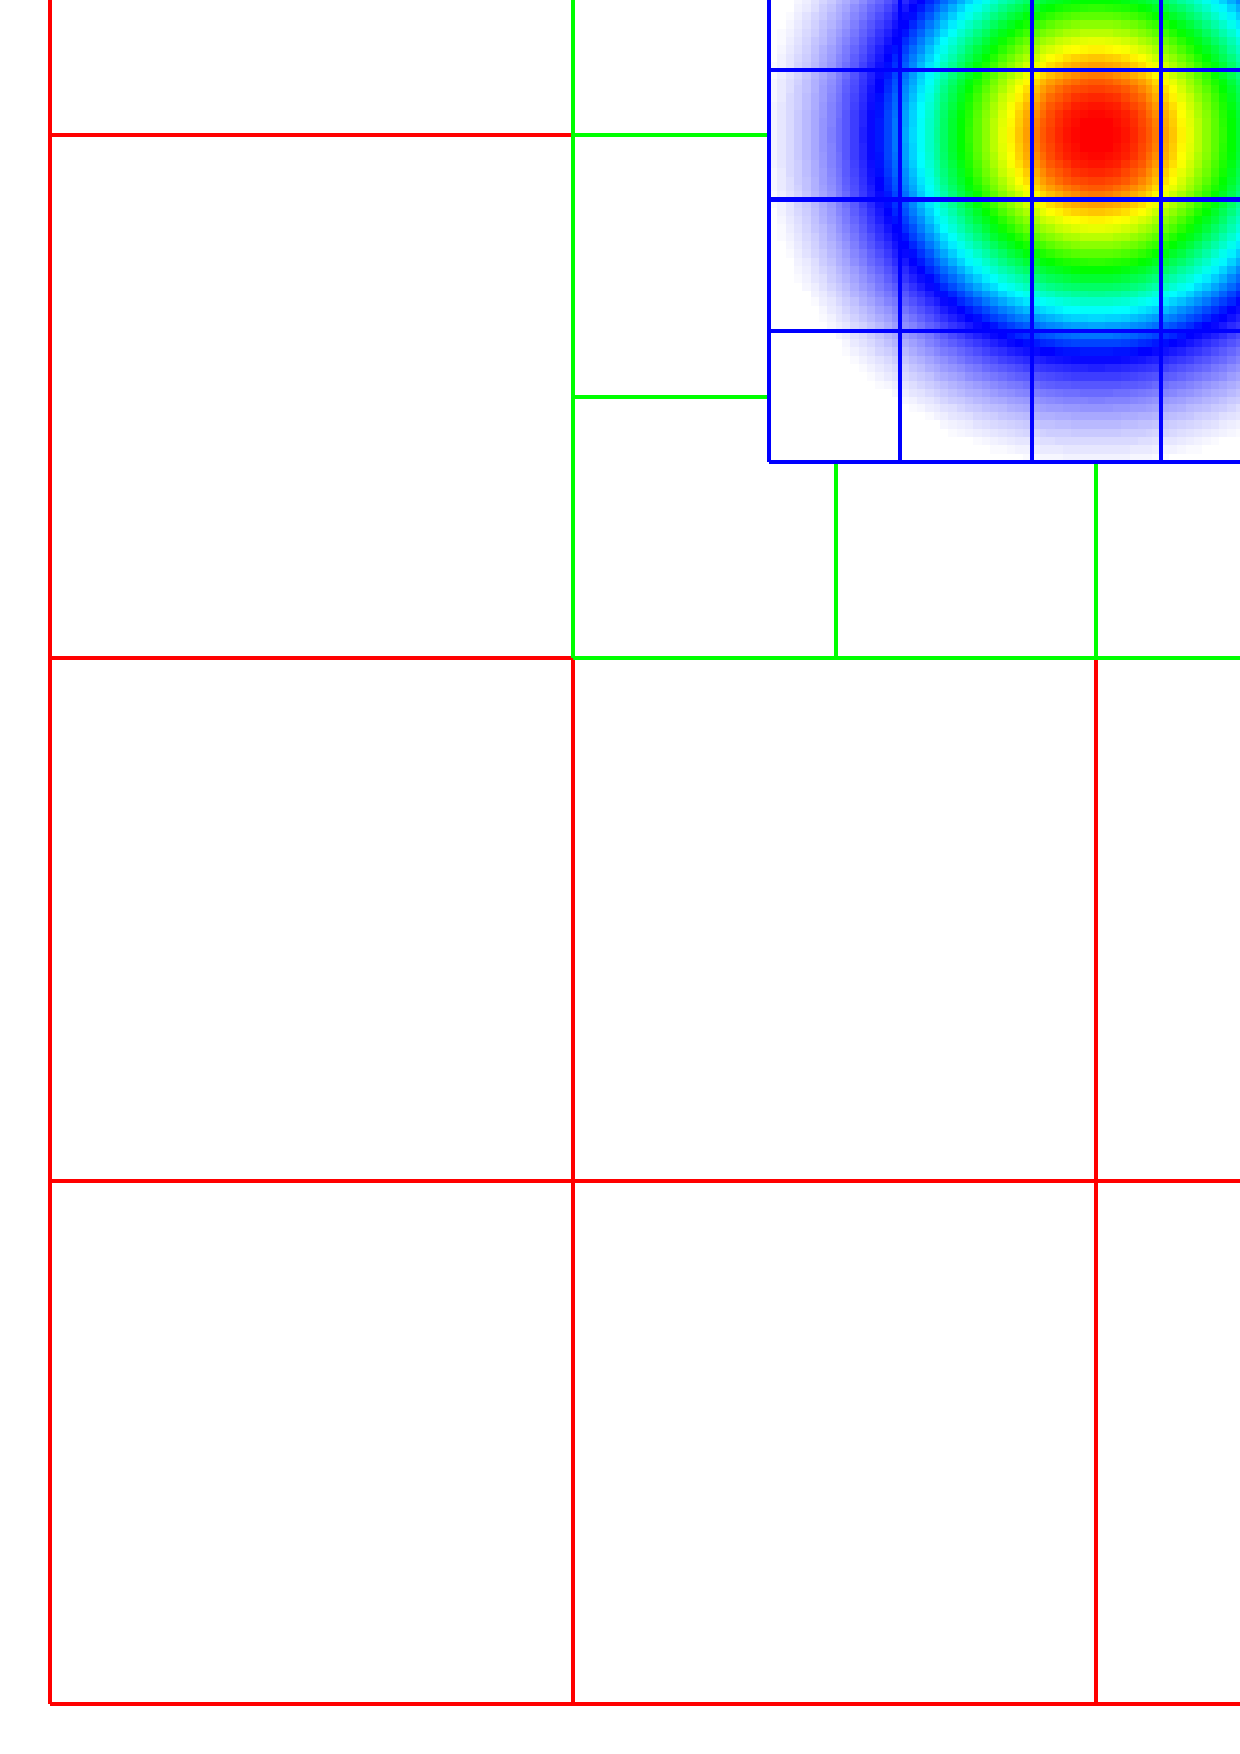
\includegraphics[width=1in]{./AmrCore/figs/Adv1.pdf}
  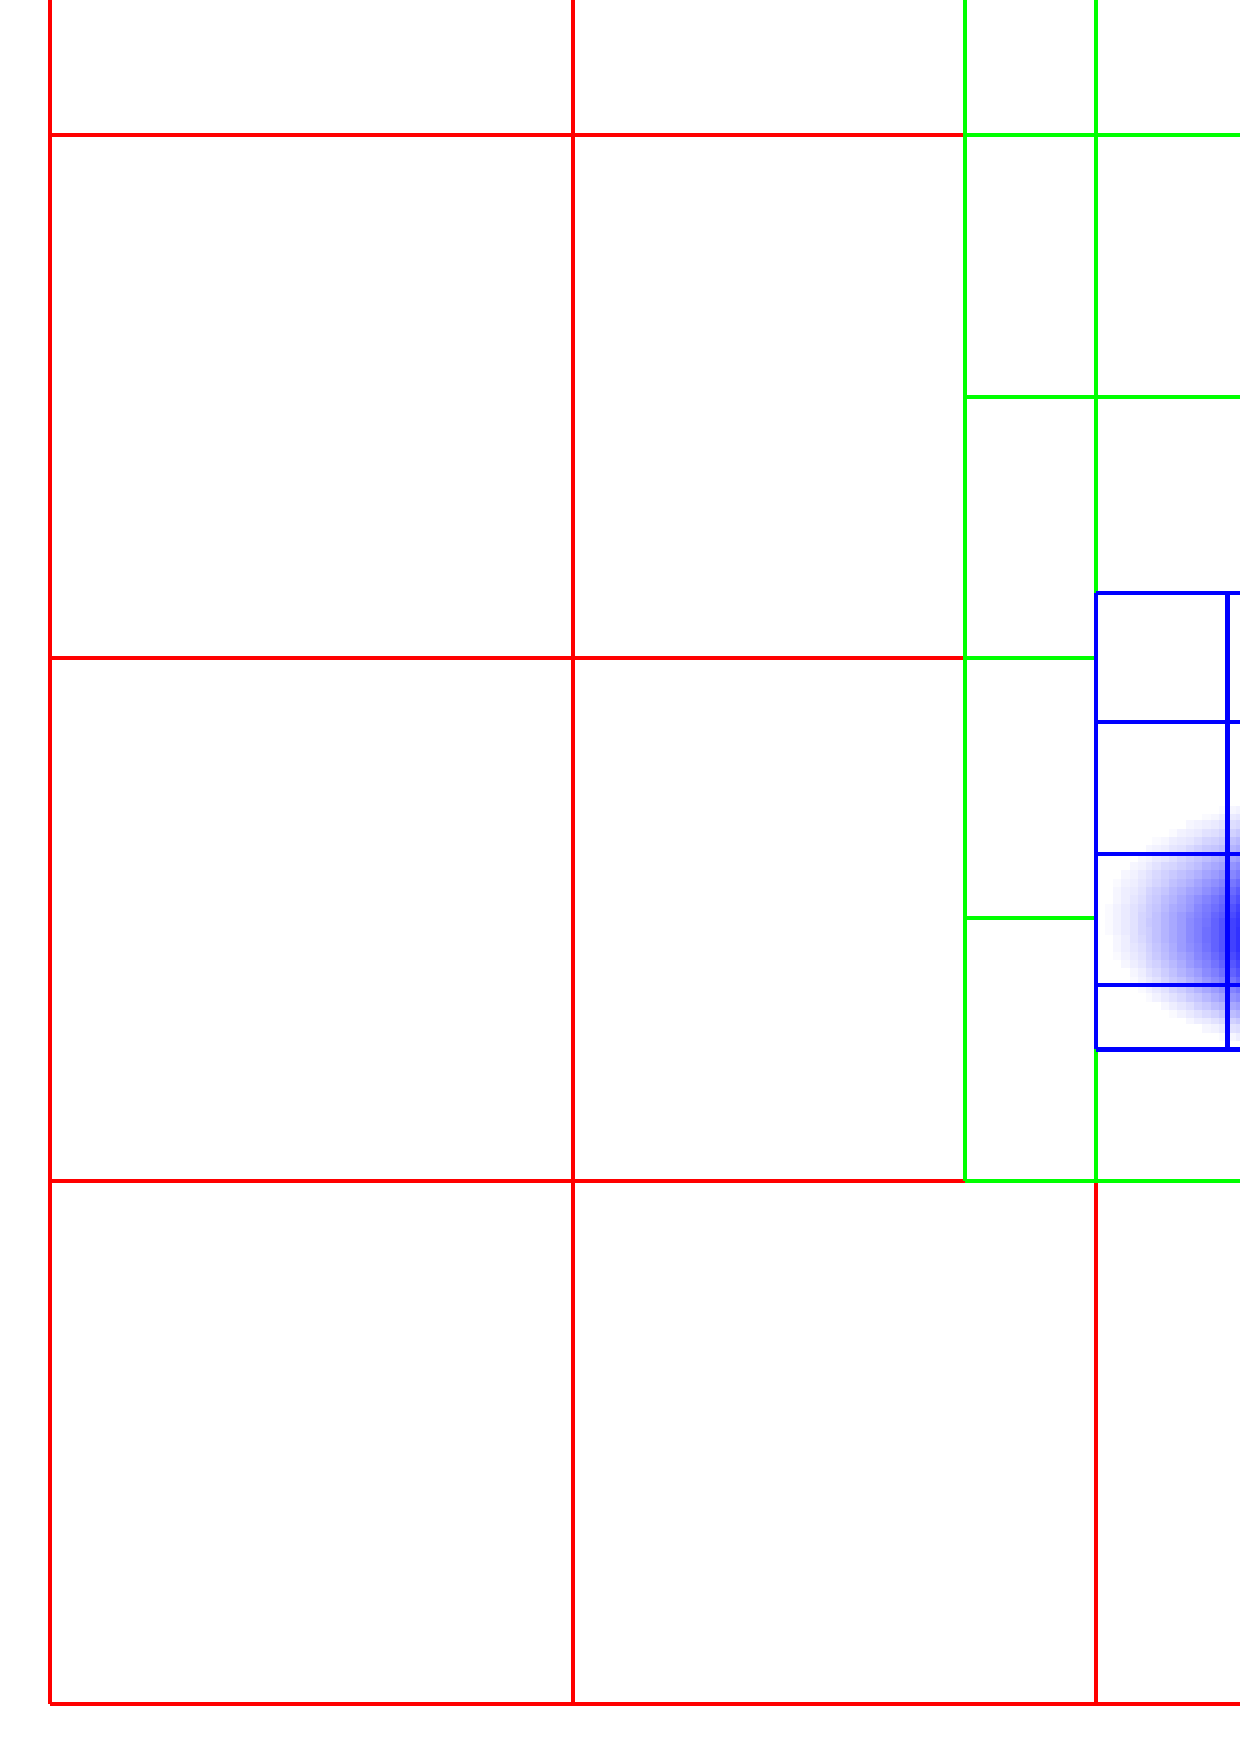
\includegraphics[width=1in]{./AmrCore/figs/Adv2.pdf}
  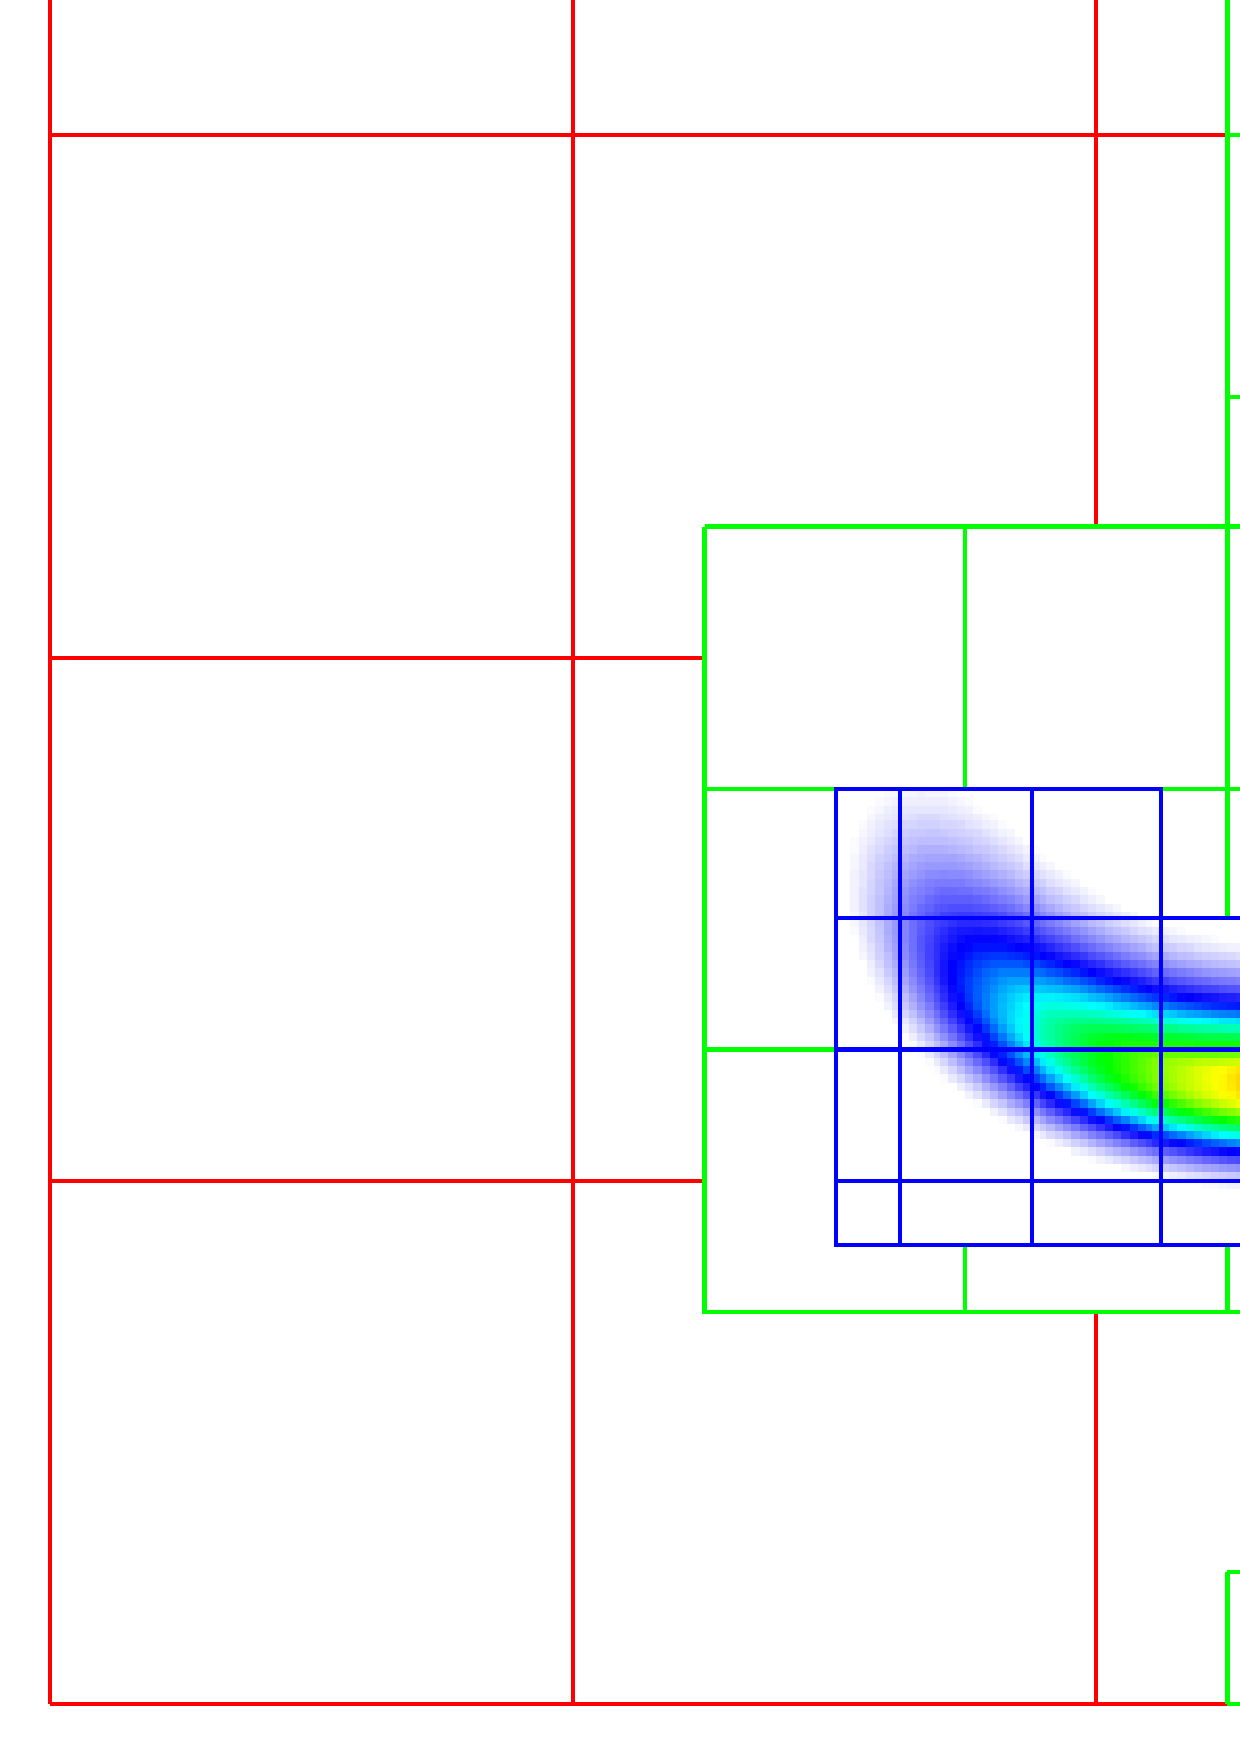
\includegraphics[width=1in]{./AmrCore/figs/Adv3.pdf}
  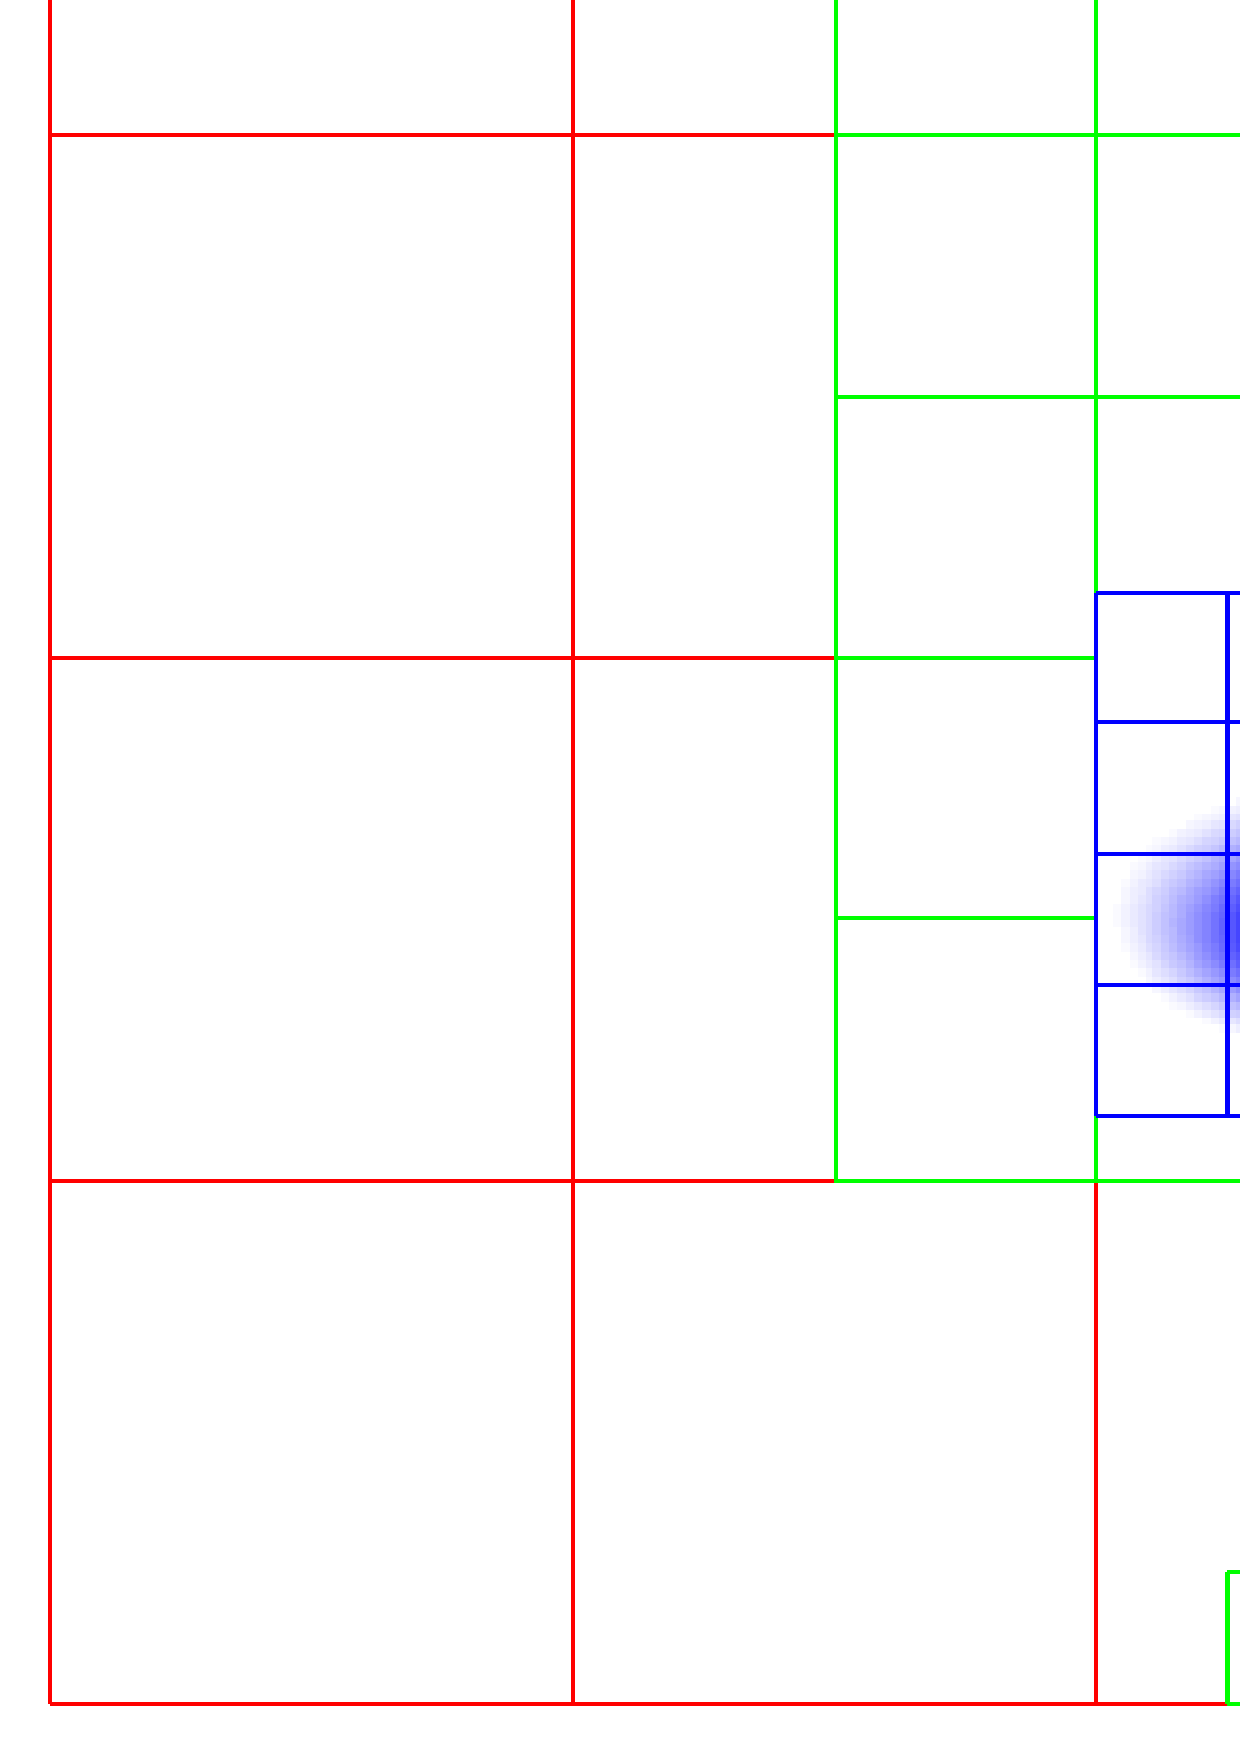
\includegraphics[width=1in]{./AmrCore/figs/Adv4.pdf}
  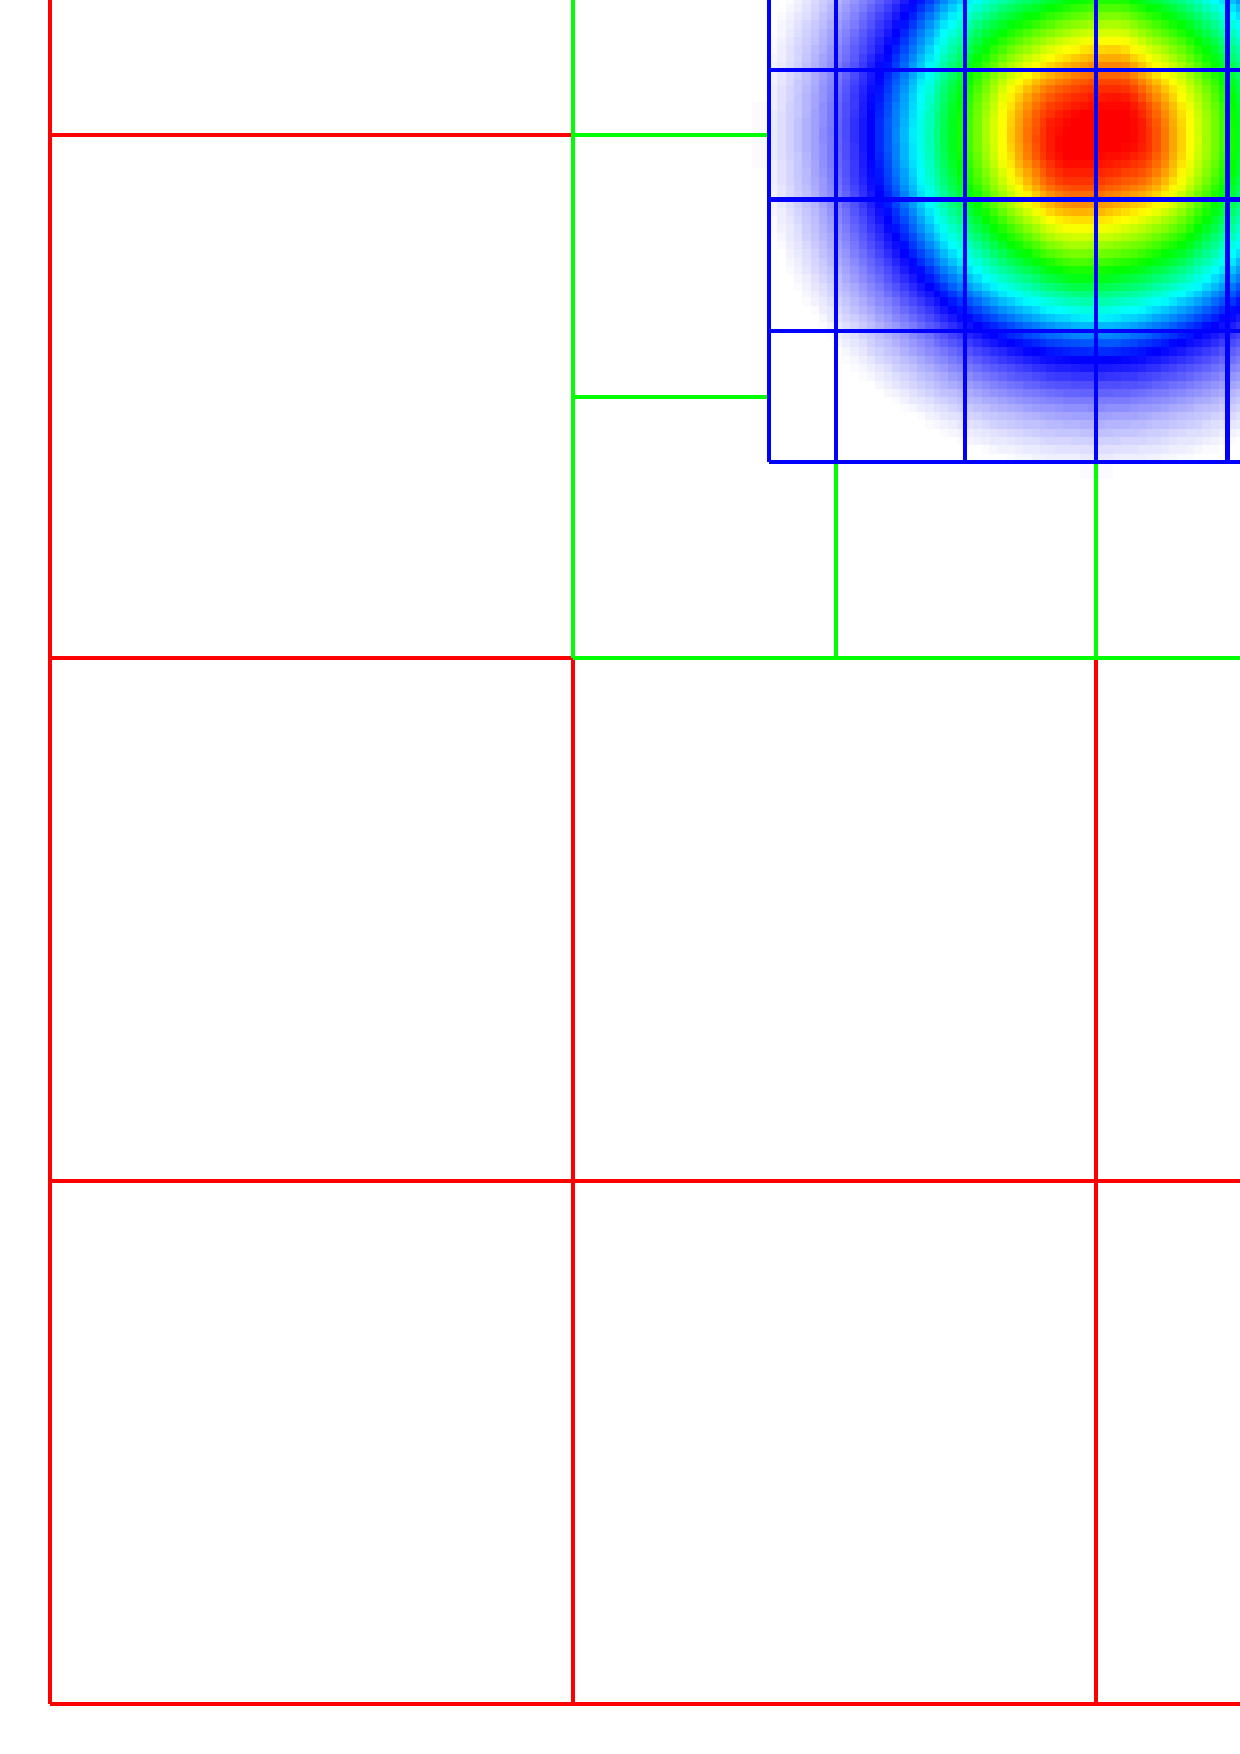
\includegraphics[width=1in]{./AmrCore/figs/Adv5.pdf}
  \caption{\label{fig:Adv} Time sequence ($t=0,0.5,1,1.5,2$~s) of advection of a Gaussian profile using the 
{\tt SingleVortex} tutorial.  The red, green, and blue boxes indicate grids at AMR levels $\ell=0,1$, and $2$.}
\end{figure}

\section{The Advection Equation}
We seek to solve the advection equation on a multi-level, adaptive grid structure:
\begin{equation}
\frac{\partial\phi}{\partial t} = -\nabla\cdot(\phi{\bf U}).
\end{equation}
The velocity field is a specified divergence-free (so the flow field is incompressible)
function of space and time.  The initial scalar field is a
Gaussian profile.  To integrate these equations on a given level, we use a simple conservative update,
\begin{equation}
\frac{\phi_{i,j}^{n+1}-\phi_{i,j}^n}{\Delta t} = \frac{(\phi u)_{i+\myhalf,j}^{n+\myhalf}-(\phi u)_{i-\myhalf,j}^{n+\myhalf}}{\Delta x} + \frac{(\phi v)_{i,j+\myhalf}^{n+\myhalf} - (\phi v)_{i,j-\myhalf}^{n+\myhalf}}{\Delta y},
\end{equation}
where the velocities on faces are prescribed functions of space and time, and the scalars on faces
are computed using a Godunov advection integration scheme.  The fluxes in this case are the face-centered,
time-centered ``$\phi u$'' and ``$\phi v$'' terms.

We use a subcycling-in-time approach where finer levels are advanced with smaller
time steps than coarser levels, and then synchronization is later performed between levels.
More specifically, the multi-level procedure can most
easily be thought of as a recursive algorithm in which, to advance level $\ell$,
$0\le\ell\le\ell_{\rm max}$, the following steps are taken:
\begin{itemize}
\item Advance level $\ell$ in time by one time step, $\Delta t^{\ell}$, as if it is
the only level.  If $\ell>0$, obtain boundary data (i.e. fill the level $\ell$ ghost cells)
using space- and time-interpolated data from the grids at $\ell-1$ where appropriate.
\item If $\ell<\ell_{\rm max}$
\begin{itemize}
\item Advance level $(\ell+1)$ for $r$ time steps with $\Delta t^{\ell+1} = \frac{1}{r}\Delta t^{\ell}$.
\item Synchronize the data between levels $\ell$ and $\ell+1$.
\end{itemize}
\end{itemize}
Specifically, for a 3-level simulation, depicted graphically in Figure \ref{fig:subcycling}:
\begin{enumerate}
\item Integrate $\ell=0$ over $\Delta t$.
\item Integrate $\ell=1$ over $\Delta t/2$.
\item Integrate $\ell=2$ over $\Delta t/4$.
\item Integrate $\ell=2$ over $\Delta t/4$.
\item Synchronize levels $\ell=1,2$.
\item Integrate $\ell=1$ over $\Delta t/2$.
\item Integrate $\ell=2$ over $\Delta t/4$.
\item Integrate $\ell=2$ over $\Delta t/4$.
\item Synchronize levels $\ell=1,2$.
\item Synchronize levels $\ell=0,1$.
\end{enumerate}
%%%%%%%%%%%%%%%%%%%%%%%%%%%%%
\begin{figure}[htb]
\begin{center}
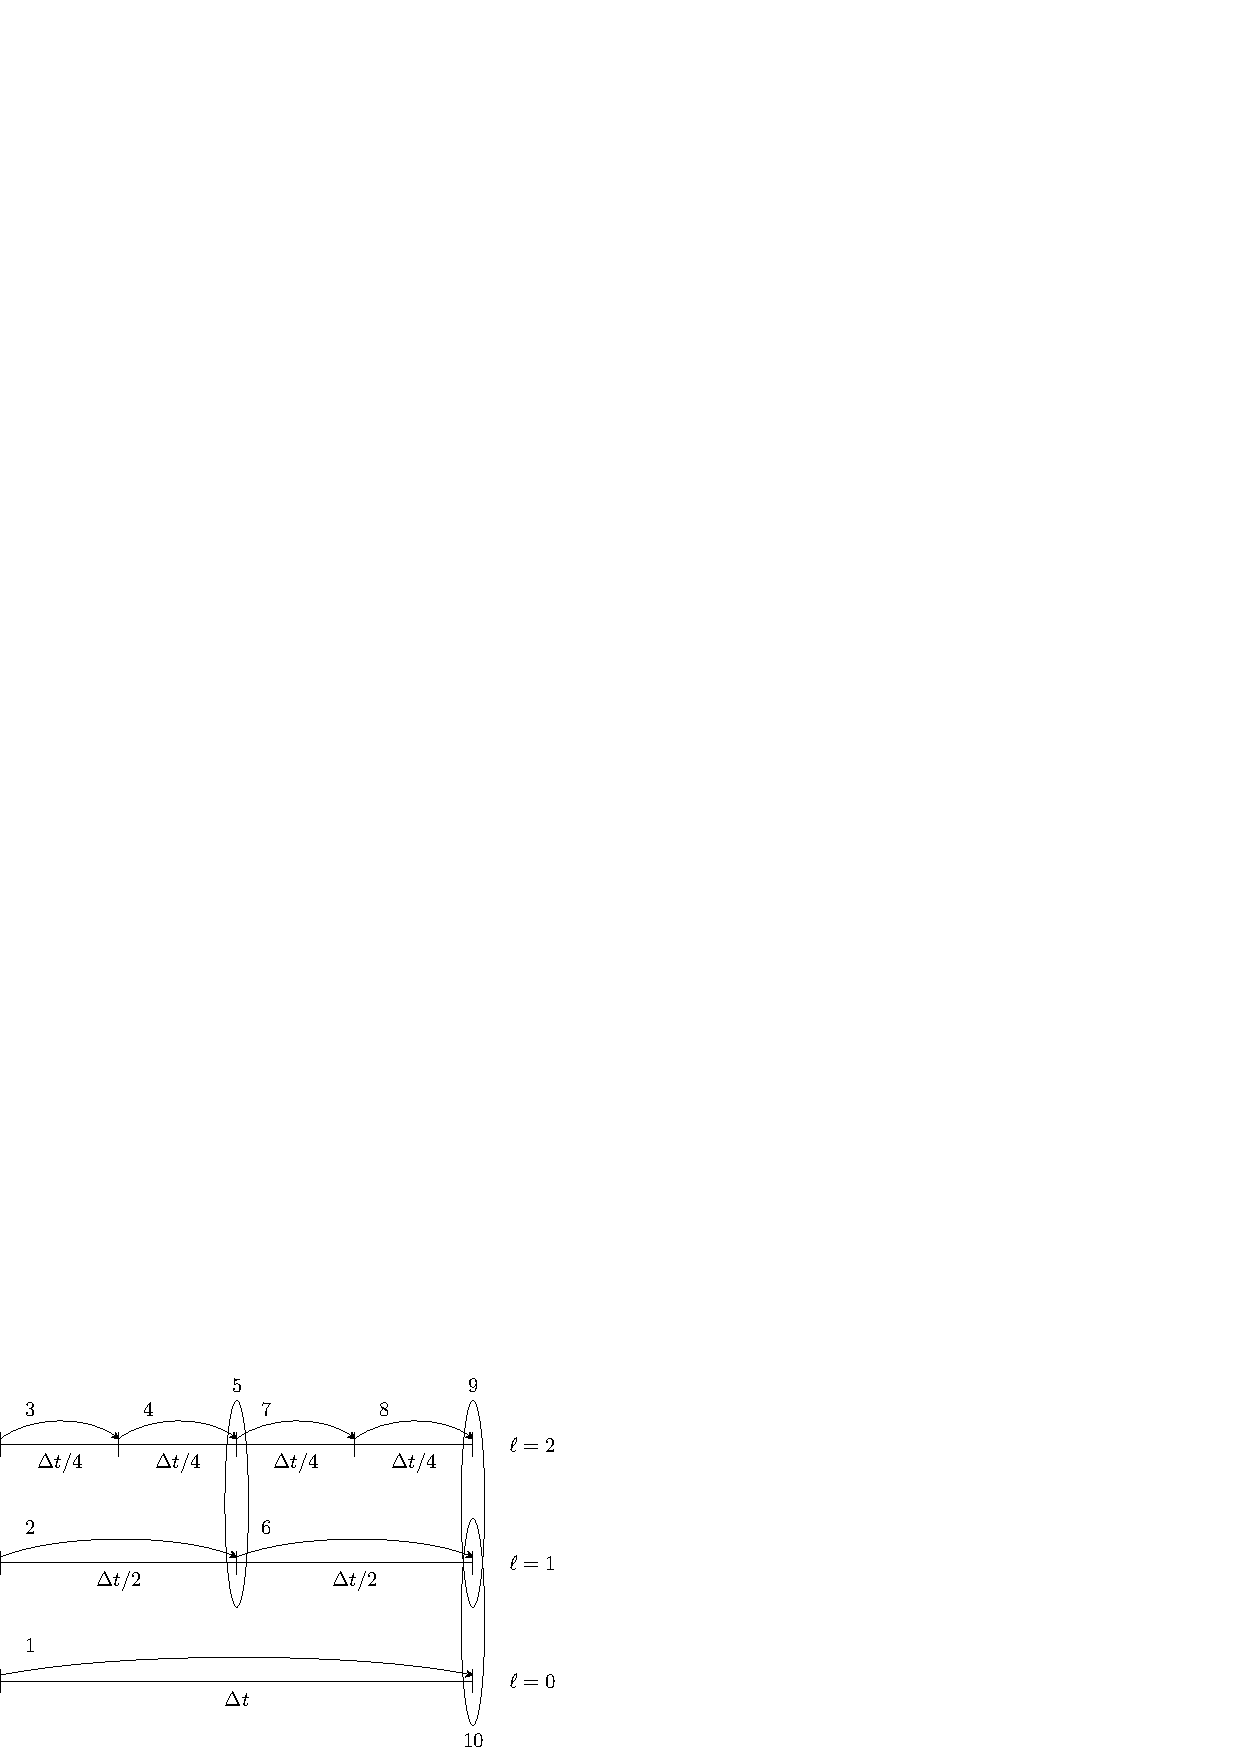
\includegraphics[width=4in]{./AmrCore/figs/subcycling.pdf}
\caption{\label{fig:subcycling} Schematic of subcycling-in-time algorithm.}
\end{center}
\end{figure}
%%%%%%%%%%%%%%%%%%%%%%%%%%%%%
For the scalar field, we keep track volume and time-weighted fluxes at coarse-fine interfaces.
We accumulate area and time-weighted fluxes in {\tt FluxRegister} objects, which can be
thought of as special boundary {\tt FABset}s associated with coarse-fine interfaces.

The idea behind the level $\ell/(\ell+1)$ synchronization step is to correct for sources of mismatch in the composite solution:
\begin{enumerate}
\item The data at level $\ell$ that underlie the level  $\ell+1$ data are not synchronized with the level $\ell+1$ data.
This is simply corrected by overwriting covered coarse cells to be the average of the overlying fine cells.
\item The area and time-weighted fluxes from the level $\ell$ faces and the level $\ell+1$ faces
do not agree at the $\ell/(\ell+1)$ interface, resulting in a loss of conservation.  
The remedy is to modify the solution in the coarse cells immediately next to the coarse-fine interface
to account for the mismatch stored in the flux register (computed by taking the coarse-level divergence of the
flux register data).
\end{enumerate}

\section{{\tt AmrCore} Source Code}
Here we provide a high-level overview of the source code in {\tt amrex/Src/AmrCore}.

\subsection{{\tt AmrMesh} and {\tt AmrCore}}

For single-level simulations
(see e.g., {\tt amrex/Tutorials/Basic/HeatEquation\_EX1\_C/main.cpp})
the user needs to build {\tt Geometry}, {\tt DistributionMapping},
and {\tt BoxArray} objects associated with the simulation.  For simulations
with multiple levels of refinement, the {\tt AmrMesh} class can be thought
of as a container to store arrays of these objects (one for each level), and
information about the current grid structure.

{\tt amrex/Src/AmrCore/AMReX\_AmrMesh.cpp/H} contains the {\tt AmrMesh} class.
The protected data members are:
\begin{lstlisting}[language=cpp]
protected:
    int            verbose;
    int            max_level;       // Maximum allowed level.
    Array<IntVect> ref_ratio;       // Refinement ratios [0:finest_level-1]

    int            finest_level;    // Current finest level.

    Array<int>     n_error_buf;     // Buffer cells around each tagged cell.
    Array<int>     blocking_factor; // Blocking factor in grid generation 
                                    // (by level).
    Array<int>     max_grid_size;   // Maximum allowable grid size (by level).
    Real           grid_eff;        // Grid efficiency.
    int            n_proper;        // # cells required for proper nesting.

    bool use_fixed_coarse_grids;
    int  use_fixed_upto_level;
    bool refine_grid_layout;        // chop up grids to have the number of 
                                    // grids no less the number of procs

    Array<Geometry>            geom;
    Array<DistributionMapping> dmap;
    Array<BoxArray>            grids;    
\end{lstlisting}

{\tt AMReX\_AmrCore.cpp/H} contains the class {\tt AmrCore}, which is derived from
the {\tt AmrMesh} class.

There are 5 pure virtual functions in the {\tt AmrCore} class:

\begin{lstlisting}[language=cpp]
//! Tag cells for refinement.  TagBoxArray tags is built on level lev grids.
virtual void ErrorEst (int lev, TagBoxArray& tags, Real time, 
                       int ngrow) override = 0;

//! Make a new level from scratch using provided BoxArray and DistributionMapping.
//! Only used during initialization.
virtual void MakeNewLevelFromScratch (int lev, Real time, const BoxArray& ba, 
                                      const DistributionMapping& dm) override = 0;

//! Make a new level using provided BoxArray and DistributionMapping and fill 
//  with interpolated coarse level data.
virtual void MakeNewLevelFromCoarse (int lev, Real time, const BoxArray& ba, 
                                     const DistributionMapping& dm) = 0;

//! Remake an existing level using provided BoxArray and DistributionMapping 
//  and fill with existing fine and coarse data.
virtual void RemakeLevel (int lev, Real time, const BoxArray& ba, 
                          const DistributionMapping& dm) = 0;

//! Delete level data
virtual void ClearLevel (int lev) = 0;
\end{lstlisting}
Refer to the {\tt AmrAdv} class in the {\tt amrex/Tutorials/Amr/AmrCore\_Advection/Source} code for a sample implementation.

\subsection{{\tt TagBox}, and {\tt Cluster}}
These classes are used in the grid generation process.  They are largely
hidden from any application codes.

The {\tt TagBox} class is essentially a data structure that marks which
cells are ``tagged'' for refinement.

{\tt Cluster} (and {\tt ClusterList} contained within the same file) are classes
that help sort tagged cells and generate a grid structure that contains all
the tagged cells.



\subsection{{\tt FillPatchUtil}}\label{sec:amrcore:fillpatch}

Many codes, including the {\tt Advection\_AmrCore} example, contain an array of {\tt MultifFab}s
(one for each level of refinement), and then use ``fillpatch'' operations to fill temporary
multifabs that have ghost cells that have been properly filled.  At the coarsest level,
the interior and domain boundary (which can be periodic or prescribed based on physical considerations)
need to be filled.  At the non-coarsest level, the ghost cells can also be interior or domain,
but can also be at coarse-fine interfaces away from the domain boundary.
{\tt AMReX\_FillPatchUtil.cpp/H} contains two primary functions of interest.
\begin{enumerate}
\item {\tt FillPatchSingleLevel()} fills a {\tt MultiFab} and its ghost region at a single level of 
refinement.  The routine is flexible enough to interpolate in time between two {\tt MultiFab}s
associated with different times.
\item {\tt FillPatchTwoLevels()} fills a {\tt MultiFab} and its ghost region at a single level of 
refinement, assuming there is an underlying coarse level.  This routine is flexible enough to interpolate
the coarser level in time first using {\tt FillPatchSingleLevel()}.
\end{enumerate}

\subsection{{\tt Interpolater}}

{\tt AMReX\_Interpolater.cpp/H} contains the virtual base class {\tt Interpolater}, which provides
an interface for coarse-to-fine spatial interpolation operators.  Thefillpatch routines describe
above require an interpolator for {\tt FillPatchTwoLevels()}
Within {\tt AMReX\_Interpolater.cpp/H} are the derived classes:
\begin{itemize}
\item {\tt NodeBilinear}
\item {\tt CellBilinear}
\item {\tt CellConservativeLinear}
\item {\tt CellConservativeProtected}
\item {\tt CellQuadratic}
\item {\tt PCInterp}
\item {\tt CellConservativeQuartic}
\end{itemize}
The fortran routines that perform the actual work associated with {\tt Interpolater} are 
contained in the files {\tt AMReX\_INTERP\_F.H} and {\tt AMReX\_INTERP\_xD.F}.

\subsection{{\tt FluxRegister}}

{\tt AMReX\_FluxRegister.cpp/H} contains the class {\tt FluxRegister}, which is derived from
the class {\tt BndryRegister} (in {\tt Src/Boundary/AMReX\_BndryRegister}).
In the most general terms, a {\tt FluxRegister} is a special type of {\tt BndryRegister} that
stores and manipulates fluxes at coarse-fine interfaces.
A simple usage scenario comes from a conservative discretization of a hyperbolic system:
\begin{equation}
\frac{\partial\phi}{\partial t} = \nabla\cdot{\bf F}
\rightarrow
\frac{\phi_{i,j}^{n+1}-\phi_{i,j}^n}{\Delta t} = \frac{F_{i+\myhalf,j}-F_{i-\myhalf,j}}{\Delta x} + \frac{F_{i,j+\myhalf} - F_{i,j-\myhalf}}{\Delta y}.
\end{equation}
Consider a two-level, two-dimensional simulation.  A standard methdology for advancing the solution in 
time is to first advance the coarse grid solution ignoring the fine level, and then advance the fine 
grid solution using the coarse level only to supply boundary conditions.  At the coarse-fine interface, 
the area weighted fluxes from the fine grid advance do not in general match the underlying flux from 
the coarse grid face, resulting in a lack of conservation.  Note that for subcycling-in-time algorithms
(where for each coarse grid advance, the fine grid is advanced $r$ times using a coarse grid time step 
reduced by a factor of $r$, where $r$ is the refinement ratio), the coarse grid flux must 
be compared to the area {\it and} time-weighted fine grid fluxes.  A {\tt FluxRegister} accumulates 
and ultimately stores the net difference in fluxes between the coarse grid and fine grid advance over 
each face over a given coarse time step.  The simplest possible synchronization step is to modify
the coarse grid solution in coarse cells immediately adjacent to the coarse-fine interface are updated
to account for the mismatch stored in the {\tt FluxRegister}.

The fortran routines that perform the actual work associated with {\tt FluxRegister} are 
contained in the files {\tt AMReX\_FLUXREG\_F.H} and {\tt AMReX\_FLUXREG\_xD.F}.

\subsection{{\tt AmrParticles} and {\tt AmrParGDB}}

The {\tt AmrCore/} directory contains derived class for dealing with particles 
in a multi-level framework.  The description of the base classes
are given in Chapter \ref{Chap:Particles}.

{\tt AMReX\_AmrParticles.cpp/H} contains the classes {\tt AmrParticleContainer}
and {\tt AmrTracerParticleContainer}, which are derived from the classes
{\tt ParticleContainer} (in {\tt Src/Particle/AMReX\_Particles})
and {\tt TracerParticleContainer} (in {\tt Src/Particle/AMReX\_TracerParticles}).

{\tt AMReX\_AmrParGDB.cpp/H} contains the class {\tt AmrParGDB}, which is derived from
the class {\tt ParGDBBase} (in {\tt Src/Particle/AMReX\_ParGDB}).

\section{{\tt Advection\_AmrCore} Example}
This example uses the class {\tt AmrAdv}, which is derived from the class {\tt AmrCore} 
(which is derived from {\tt AmrMesh}).  The function definitions/implementations
are given in {\tt AmrAdv.H/cpp}.  
Here is a high-level pseudo-code of the flow of the program:
\begin{lstlisting}[language=cpp]
/* Advection_AmrCore Pseudocode */
main()
  AmrAdv amradv; // build an AmrAdv object
  amradv.InitData()  // initialize data all all levels
    AmrCore::InitFromScratch()
      AmrMesh::MakeNewGrids()
	AmrMesh::MakeBaseGrids() // define level 0 grids
	AmrAdv::MakeNewLevelFromScratch()
          /* allocate phi_old, phi_new, t_new, and flux registers */
          initdata()  // fill phi
	if (max_level > 0) {
          do {
  	    AmrMesh::MakeNewGrids()
	      /* construct next finer grid based on tagging criteria */
 	    AmrAdv::MakeNewLevelFromScratch()
              /* allocate phi_old, phi_new, t_new, and flux registers */
              initdata()  // fill phi
	  } (while (finest_level < max_level);
        }
  amradv.Evolve()
    loop over time steps {
      ComputeDt()
      timeStep() // advance a level
        /* check regrid conditions and regrid if necessary */
        Advance()
          /* copy phi into a multifab and fill ghost cells */
          /* advance phi */
          /* update flux registers */
        if (lev < finest_level) {
          timeStep() // recursive call to advance the next-finer level "r" times
            /* check regrid conditions and regrid if necessary */
            Advance()
              /* copy phi into a multifab and fill ghost cells */
              /* advance phi */
              /* update flux registers */
          reflux() // synchronize lev and lev+1 using fluxregister divergence
          AverageDown() // set covered coarse cells to be the average of fine
        }
    }
\end{lstlisting}

\subsection{{\tt FluxRegister}s}
The function {\tt AmrAdv::Advance()} calls the fortran
subroutine, {\tt advect} (in {\tt ./Src\_xd/Adv\_xd.f90}).  {\tt advect} computes
and returns the time-advanced state as well as the fluxes used to update the state.
These fluxes are used to set or increment the flux registers.
\begin{lstlisting}[language=cpp]
// increment or decrement the flux registers by area and time-weighted fluxes
// Note that the fluxes have already been scaled by dt and area
// In this example we are solving phi_t = -div(+F)
// The fluxes contain, e.g., F_{i+1/2,j} = (phi*u)_{i+1/2,j}
// Keep this in mind when considering the different sign convention for updating
// the flux registers from the coarse or fine grid perspective
// NOTE: the flux register associated with flux_reg[lev] is associated
// with the lev/lev-1 interface (and has grid spacing associated with lev-1)
if (do_reflux) { 
   if (flux_reg[lev+1]) {
      for (int i = 0; i < BL_SPACEDIM; ++i) {
          flux_reg[lev+1]->CrseInit(fluxes[i],i,0,0,fluxes[i].nComp(), -1.0);
      }	    
   }
   if (flux_reg[lev]) {
      for (int i = 0; i < BL_SPACEDIM; ++i) {
          flux_reg[lev]->FineAdd(fluxes[i],i,0,0,fluxes[i].nComp(), 1.0);
      }
   }
}
\end{lstlisting}
The synchronization is performed at the end of {\tt AmrAdv::timeStep}:
\begin{lstlisting}[language=cpp]
if (do_reflux)
{
    // update lev based on coarse-fine flux mismatch
    flux_reg[lev+1]->Reflux(*phi_new[lev], 1.0, 0, 0, phi_new[lev]->nComp(),
                            geom[lev]);
}

AverageDownTo(lev); // average lev+1 down to lev
\end{lstlisting}

In order to define an AMR grid structure, you must define a routine that ``tags'' which
cells require refinement.  The pure virtual function {\tt ErrorEst} in the {\tt AmrMesh}
is defined in the {\tt AmrAdv} class.  The {\tt ErrorEst} function must call a subroutine
that sets elements of a {\tt TagBoxArray} to either 1 or 0.


\chapter{{\tt Amr} Source Code}\label{Chap:AmrLevel}
The source code in {\tt amrex\_Src/Amr} contains a number of classes, most notably
the {\tt Amr}, {\tt AmrLevel}, and {\tt LevelBld}.
The {\tt Amr} class is derived from {\tt AmrCore}, and manages data across the 
entire AMR hierarchy of grids.
The {\tt AmrLevel} class is a pure virtual class for managing data at a
single level of refinement.
The {\tt LevelBld} class is a pure virtual class for defining variable types
and attributes.

Many of our mature application codes contain derived classes that inherit directly
from {\tt AmrLevel}.  These include our compressible astrophysics code,
{\tt CASTRO}, and our computational cosmology code, {\tt NYX}.  We also have
NYX for computational cosmology)   We also have 
a pure virtual class called {\tt NavierStokesBase} that inherits from {\tt AmrLevel}
(available in the {\tt AMReX-codes/IAMR} github repository).  Our incompressible
Navier-Stokes code, {\tt IAMR}, as well as our low Mach number combustion code,
{\tt PeleLM}, inherit from {\tt NavierStokesBase}.

The tutorial code in {\tt amrex/Tutorials/Amr/Advection\_AmrLevel} gives a simple
example of a class derived from {\tt AmrLevel} that can be used to solve
the advection equation on a subcycling-in-time AMR hierarchy.  Note that example
is essentially the same as the {\tt amrex/Tutorials/Amr/Advection\_AmrCore} tutorial
and documentation in Chatper \ref{Chap:AmrCore}, except now we use the provided
libraries in {\tt Src/Amr}.

The most important data managed by the {\tt AmrLevel} is an array of {\tt StateData},
which holds the scalar fields, etc., in the boxes that together make up the level.

\section{{\tt StateData}}
{\tt StateData} is a class that essentially holds a pair of {\tt MultiFab}s: one at the old time and one
at the new time. {\tt AMReX} knows how to interpolate in time between these states to get data at
any intermediate point in time. The main data that we care about in our applications codes 
(such as the fluid state) will be stored as {\tt StateData}. Essentially, data is made {\tt StateData}
if we need it to be stored in checkpoints / plotfiles, and/or we want it to be automatically
interpolated when we refine.
An {\tt AmrLevel} stores an array of {\tt StateData} (in a C ++ array called state). We index this array
using integer keys (defined via an enum in, e.g., {\tt AmrLevelAdv.H}):
\begin{lstlisting}[language=cpp]
enum StateType { Phi_Type = 0,
                 NUM_STATE_TYPE };
\end{lstlisting}
In our tutorial code, we use the function {\tt AmrLevelAdv::variableSetup} to tell our simulation about
the {\tt StateData} (e.g., how many variables, ghost cells, nodality, etc.)
Note that if you have more than one {\tt StateType}, each of the different {\tt StateData} 
carried in the state array can have different numbers
of components, ghost cells, boundary conditions, etc. This is the main reason we separate all this
data into separate {\tt StateData} objects collected together in an indexable array.

\section{{\tt Advection\_AmrLevel} Example}

Figure \ref{fig:AmrAdvection_AmrLevel_flowchart} shows a source
code tree for the {\tt AmrAdvection\_AmrLevel} example.
%%%%%%%%%%%%%%%%%%%%%%%%%%%%%
\begin{figure}[htb]
\begin{center}
\includegraphics[width=4in]{./AmrLevel/figs/flowchart.pdf}
\caption{\label{fig:AmrAdvection_AmrLevel_flowchart} Source code tree for the 
         {\tt AmrAdvection\_AmrLevel} example.}
\end{center}
\end{figure}
%%%%%%%%%%%%%%%%%%%%%%%%%%%%%
\begin{itemize}
\item {\tt amrex/Src/}
\begin{itemize}
\item {\tt Base/} Base {\tt amrex} library.
\item {\tt Boundary/} An assortment of classes for handling boundary data.
\item {\tt AmrCore/} AMR data management classes, described in more detail above.
\item {\tt Amr/}
\item {\tt Particle/}
\end{itemize}
\item {\tt Advection\_AmrLevel/Src} Source code specific to this example.  Most notably
is the {\tt AmrLevelAdv} class, which is derived from {\tt AmrLevel}.  The subdirectories {\tt Src\_2d}
and {\tt Src\_3d} contain dimension specific routines.  {\tt Src\_nd} contains dimension-independent routines.
\item {\tt Exec} Contains a makefile so a user can write other examples besides {\tt SingleVortex} and {\tt UniformVelocity}.
\item {\tt SingleVortex} and {\tt UniformVelocity}
Build the code here by editing the {\tt GNUmakefile} and running {\tt make}.  There
is also problem-specific source code here used for initialization or specifying the velocity field used in this
simulation.
\end{itemize}

\begin{lstlisting}[language=cpp]
/* Advection_AmrLevel Pseudocode */
main()
  Amr amr;
  amr.init()
  loop { 
    amr.coarseTimeStep()
      /* compute dt */
      timeStep()
        amr_level[level]->advance()
        call timeStep r times for next-finer level
        amr_level[level]->post_timestep() // AMR synchronization
      postCoarseTimeStep()
      /* write plotfile and checkpoint */
  }
  /* write final plotfile and checkpoint */
\end{lstlisting}


\chapter{Particles}\label{Chap:Particles}
In addition to the tools for working with mesh data described in previous chapters, $\tt{AMReX}$ provides data structures and iterators for performing data-parallel particle simulations. 
Our approach is particularly suited to particles that interact with data defined on a (possibly adaptive) block-structured hierarchy of meshes. Example use cases include Particle-in-Cell
simulations, Lagrangian tracers, or particles that exert a drag force onto a fluid, such as in multi-phase flow calculations. The overall goals of $\tt{AMReX}$'s particle 
tools are to allow users flexibility in specifying how the particle data is laid out in memory and to handle the parallel communication of particle data automatically.
In the following sections, we give an overview of $\tt{AMReX}$'s particle classes and how to use them.

\section{The Particle}
\label{sec:Particles:Particle}

The particle classes can be used by including the header $\tt{AMReX\_Particles.H}$. The most basic particle data structure is the particle struct itself: 

\begin{lstlisting}[language=cpp]
  Particle<3, 2> p;
\end{lstlisting}

This is a templated data type, designed to allow users flexibility in specifying the number and type of variables that the particles carry. The first template parameter is
the number of extra $\tt{Real}$ variables this particle will have (either single or double precision), while the second is the number of extra integer variables. It is imporant to note
that this is the number of $\emph{extra}$ real and integer variables; a particle will always have at least $\tt{BL\_SPACEDIM}$ $\tt{Real}$ components that store the particle's position
and $\tt{2}$ integer components that store the particle's $\tt{id}$ and $\tt{cpu}$ numbers.
\footnote{Note that $\tt{cpu}$ stores the number of the process the particle was $\emph{generated}$
on, not the one its currently assigned to. This number is set on initialization and never changes, just like the particle $\tt{id}$. In essence, the particles have two integer id numbers, and only the combination of the two is unique. This was done to facilitate the creation of particle initial conditions in parallel.}

The particle struct is designed to store these variables in a way that minimizes padding, which in practice means that the $\tt{Real}$ components always come first, and the integer
components second. Additionally, the required particle variables are stored before the optional ones, for both the real and the integer components. For example, say we want to define
a particle type that stores a mass, three velocity components, and two extra integer flags. Our particle struct would be set up like:

\begin{lstlisting}[language=cpp]
  Particle<4, 2> p;
\end{lstlisting}

and the order of the particle components in would be: x y z m vx vy vz id cpu flag1 flag2. \footnote{Note that for the extra particle components, which component refers to which
variable is an application-specific convention - the particles have 4 extra real comps, but which one is ``mass'' is up to the user. We suggest using an \tt{enum} to keep these indices straight; please see Section~\ref{sec:Particles:Initializing} below for an example of this.} 

\subsection{Setting Particle data}

The $\tt{Particle}$ struct provides a number of methods for getting and setting a particle's data. For the required particle components, there are special, named methods. For the 
``extra'' real and integer data, you can use the $\tt{rdata}$ and $\tt{idata}$ methods, respectively. 

\begin{lstlisting}[language=cpp]
  Particle<2, 2> p;

  p.pos(0) = 1.0;
  p.pos(1) = 2.0;
  p.pos(2) = 3.0;
  p.id() = 1;
  p.cpu()  = 0;

  // p.rdata(0) is the first extra real component, not the 
  // first real component overall
  p.rdata(0) = 5.0;
  p.rdata(1) = 5.0;

  // and likewise for p.idata(0);
  p.rdata(0) = 17;
  p.idata(1) = -64;  
\end{lstlisting}

\section{The ParticleContainer}
\label{sec:Particles:ParticleContainer}
 
One particle by itself is not very useful. To do real calculations, a collection of particles needs to be defined, and the location of the particles within the AMR hierarchy
(and the corresponding MPI process) needs to be tracked as the particle positions change. To do this, we provide the $\tt{ParticleContainer}$ class:

\begin{lstlisting}[language=cpp]
  ParticleContainer<3, 2, 4, 4> mypc;
\end{lstlisting}
   
\subsection{Arrays-of-Structs and Structs-of-Arrays}

Like the $\tt{Particle}$ class itself, the $\tt{ParticleContainer}$ class is templated. The first two template parameters have the same meaning as before: they define the number of each type of variables that the particles in this container will store. In addition, there are two more optional template parameters that allow the user to specify additional particle
variables that will be stored in Struct-of-Array form. The difference between Array-of-Struct and Struct-of-Array data is in how the data is laid
out in memory. For the Array-of-Struct data, all the variables associated with particle 1 are next to each other in memory, followed by all the variables associated with particle
2, and so on. For variables stored in Struct-of-Array style, all the particle data for a given component is next to each other in memory, and each component is stored in a seperate
array. For convenience, we (arbitrarily) refer to the components in the particle struct as particle $\emph{data}$, and components stored in the Struct-of-Arrays as particle
$\emph{attributes}$. See Figure XXX for an illustration.

To see why the distinction between Array-of-Struct and Struct-of-Array data is important, consider the following extreme case. Say you have particles that carry 100 different components,
but that most of the time, you only need to do calculations involving 3 of them (say, the particle positions) at once. In this case, storing all 100 particle variables in the particle
struct is clearly inefficient, since most of the time you are reading 97 extra variables into cache that you will never use. By splitting up the particle variables into stuff that gets 
used all the time (stored in the Array-of-Structs) and stuff that only gets used infrequently (stored in the Struct-of-Arrays), you can in principle acheive much better cache reuse. Of course, the usage pattern of your application likely won't be so clear-cut. Flexibility in how the particle data is stored also makes it easier to interface between $\tt{AMReX}$ and already-existing Fortran subroutines.

Note that while ``extra'' particle data can be stored in either Struct-of-Array or Array-of-Struct style, the particle positions and id numbers are $\emph{always}$ stored in the particle
structs. This is because these particle variables are special and used internally by $\tt{AMReX}$ to assign the particles to grids and to mark particles as valid or invalid, respectively.

\subsection{Constructing ParticleContainers}

A particle container is always associated with a particular set of AMR grids and a particular set of $\tt{DistributionMap}$s that describes which MPI processes those grids live on.
For example, if you only have one level, you can define a $\tt{ParticleContainer}$ to store particles on that level using the following constructor:

\begin{lstlisting}[language=cpp]
    ParticleContainer (const Geometry            & geom,
                       const DistributionMapping & dmap,
                       const BoxArray            & ba);
\end{lstlisting}

Or, if you have multiple levels, you can use following constructor instead:

\begin{lstlisting}[language=cpp]
    ParticleContainer (const Array<Geometry>            & geom,
                       const Array<DistributionMapping> & dmap,
                       const Array<BoxArray>            & ba,
                       const Array<int>                 & rr);
\end{lstlisting}

Note the set of grids used to define the $\tt{ParticleContainer}$ doesn't have to be the same set used to define the simulation's mesh data. However, it is often desirable to have
the two hierarchies track each other. If you are using an $\tt{AmrCore}$ class in your simulation (see Chapter~\ref{Chap:AmrCore}), you can achieve this by using 
the $\tt{AmrParticleContainer}$ class. The constructor for this class takes a pointer to your $\tt{AmrCore}$ derived class, instead:

\begin{lstlisting}[language=cpp]
  AmrTracerParticleContainer (AmrCore* amr_core);
\end{lstlisting}

In this case, the $\tt{Array<BoxArray>}$ and $\tt{Array<DistributionMap>}$ used by your $\tt{ParticleContainer}$ will be updated automatically to match those in
your $\tt{AmrCore}$. 

The $\tt{ParticleContainer}$ stores the particle data in a manner prescribed by the set of AMR grids used to define it. If tiling is turned off, then every grid has its own 
Array-of-Structs and Struct-of-Arrays. Which AMR grid a particle is assigned to is determined by examining its position and binning it, using the domain left edge as an offset. 
By default, a particle is assigned to the finest level that contains its position, although this behavior can be tweaked (see Section~\ref{sec:Particles:Subcycling} below). 
When tiling is enabled, then each $\emph{tile}$ gets its own Struct-of-Arrays and Array-of-Structs instead. Note that this is different than what happens with mesh data. With mesh
data, the tiling is strictly logical; the data is laid out in memory the same whether tiling is turned on or off. With particle data, however, the particles are actually stored in 
a different arrays when tiling is enabled. As with mesh data, the particle tile size can be tuned so that an entire tile's worth of particles will fit into a cache line at once.

Once the particles move, their data may no longer be in the right place in the container. They can be reassigned by calling the $\tt{Redistribute()}$ method of $\tt{ParticleContainer}$.
After calling this method, all the particle will be moved to their proper places in the container, and all invalid particles (particles with id set to $-1$) will be removed. All the 
MPI communication needed to this happens automatically; their is no need for application developers to worry about communicating particle data themselves.

As you build your application, you will likely want to create your own derived $\tt{ParticleContainer}$ class that specializes the template parameters and adds additional 
functionality, like setting the particle initial conditions, moving the particles, etc. See Section~\ref{sec:Particles:Initializing} for an example.

\section{Initializing Particle Data}
\label{sec:Particles:Initializing}

In the following code snippet, we create a derived particle container with 2 real components and 2 integer components, both stored in the Struct-of-Arrays.
We give our derived class an $\tt{InitParticles}$ method that creates one particle per cell on the coarse level, and shows how to set the particle attributes
and add them to the proper container. 

\begin{lstlisting}[language=cpp]

  // These enums are used to keep track of what index means what
  // for the real... 
  struct RealIdx {
    enum {
      eggs = 0,
      ham,
      nattribs
    };
  };
  
  // ... and the integer attributes.
  struct IntIdx {
    enum {
      foo = 0,
      bar,
      nattribs
    };
  };

  // Now we define our ParticleContainer subclass, 
  // passing in the appropriate template parameters.
  class MyParticleContainer
  : public ParticleContainer<0, 0,
                             RealIdx::nattribs,
                             IntIdx::nattribs>
  {
    public:
    
    MyParticleContainer (const Array<Geometry>            & geom,
                         const Array<DistributionMapping> & dmap,
                         const Array<BoxArray>            & ba,
                         const Array<int>                 & rr)
        : ParticleContainer<0, 0,
                            RealIdx::nattribs,
                            IntIdx::nattribs> (geom, dmap, ba, rr) {}

    void InitParticles() {
        const int lev = 0;
        const Geometry& geom = Geom(lev);
        const Real* dx  = geom.CellSize();

        ParticleType p;
        for (MFIter mfi = MakeMFIter(lev); mfi.isValid(); ++mfi) {
            const Box& tile_box = mfi.tilebox();
            const RealBox tile_real_box { tile_box, dx, geom.ProbLo() };

            const int grid_id = mfi.index();
            const int tile_id = mfi.LocalTileIndex();
            auto& particle_tile = GetParticles(lev)[std::make_pair(grid_id, 
                                                                   tile_id)];

            const auto& boxlo = tile_box.smallEnd();
            for (IntVect iv = tile_box.smallEnd(); iv <= tile_box.bigEnd(); 
                 tile_box.next(iv)) {

                // set the particle id and cpu (in the particle struct)
                p.id() = ParticleType::NextID();
                p.cpu() = ParallelDescriptor::MyProc();

                // set the particle positions (also in the struct)
                AMREX_D_TERM(
                p.pos(0) = tile_real_box.lo(0) + (iv[0]- boxlo[0] + 0.5)*dx[0];,
                p.pos(1) = tile_real_box.lo(1) + (iv[1]- boxlo[1] + 0.5)*dx[1];,
                p.pos(2) = tile_real_box.lo(2) + (iv[2]- boxlo[2] + 0.5)*dx[2];
                );

                // set this particle's real attributes
                // (Probably want to do something more 
                // interesting here... )
                std::array<double, RealIdx::nattribs> real_attribs;
                real_attribs[RealIdx::ham]  = 7.0;
                real_attribs[RealIdx::eggs] = 9.0;

                // set this particle's integer attributes (ditto)
                std::array<int, IntIdx::nattribs> int_attribs;
                int_attribs[IntIdx::foo]  = -1;
                int_attribs[IntIdx::bar]  = 12; 

                particle_tile.push_back(p);
                particle_tile.push_back_real(real_attribs);
                particle_tile.push_back_int(int_attribs);
            }
        }
    }
};

\end{lstlisting}

In the above code, because each process only generates particles in grids that it owns, the particles are already in the right place in the container. 
In general, however, users may need to call $\tt{Redistribute()}$ after adding particles, if the processes generate particles they don't own (for example,
if the particle positions are perturbed from the cell centers and thus end up outside their parent grid).

\section{Iterating over Particles}
\label{sec:Particles:Iterating}

To iterate over the particles on a given level in your container, you can use the $\tt{ParIter}$ class, which comes in 
both const and non-const flavors. For example:

\begin{lstlisting}[language=cpp]

for (MyParIter pti(*this, lev); pti.isValid(); ++pti) {
    auto& particles = pti.GetArrayOfStructs();
    for (unsigned i = 0; i < pti.numParticles(); ++i) {
        const ParticleType& p = particles[i];
        // do stuff with p...
    }
}
\end{lstlisting}

The outer loop will execute once every grid (or tile, if tiling is enabled) \emph{that contains particles}; grids or tiles
that don't have any particles will be skipped. 

\section{Passing particle data into Fortran routines}
\label{sec:Particles:Fortran}

Because the $\tt{AMReX}$ particle struct is a Plain-Old-Data type, it is interoperable with FORTRAN when the $\tt{bind(C)}$
attribute is used. It is therefore possible to pass a grid or tile worth of particles into fortran routines for processing,
instead of iterating over them in C++. You can also define a Fortran derived type that is equivalent to C struct used for the
particles. For example:

\begin{lstlisting}[language=fortran]

    use amrex_fort_module, only: amrex_real
    use iso_c_binding ,    only: c_int

    type, bind(C)  :: particle_t
       real(amrex_real) :: pos(3)
       real(amrex_real) :: vel(3)
       real(amrex_real) :: acc(3)
       integer(c_int)   :: id
       integer(c_int)   :: cpu
    end type particle_t

\end{lstlisting}

is equivalent to particle struct you get with $\tt{Particle<6, 0>}$.

\section{Interacting with Mesh Data}
\label{sec:Particles:Interacting}

SumBoundary. Syncing across levels. ElectrostaticPIC tutorial.

\section{Short Range Forces}
\label{sec:Particles:ShortRange}

Neighbor particles. Optional communication. The ShortRangeParticles tutorial.

\section{Particle IO}
\label{sec:Particles:IO}

IO Routines (ASCII and binary), visualization options. Converter python script.

\section{Subcycling with Particles}
\label{sec:Particles:Subcycling}

This is hard. Ghosts and Virtuals.  



\chapter{Fortran Interface}\label{Chap:Fortran}
The core of \amrex\ is written in \cpp.  For Fortran users who want to
write all of their programs in Fortran, \amrex\ provides Fortran
interfaces around most of functionalities except for particles
(Chapter~\ref{Chap:Particles}) and the {\tt AmrLevel} class
(Chapter~\ref{Chap:AmrLevel}).  We should not confuse the Fortran
interface in this chapter with the Fortran kernel functions called
inside {\tt MFIter} loops in \cpp codes
(Section~\ref{sec:basics:fortran}).  For the latter, Fortran is used
in some sense as a domain-specific language with native
multi-dimensional arrays, whereas here Fortran is used to drive the
whole application code.  In order to better understand \amrex, Fortran
interface users should read the rest of the User's Guide except for
Chapters~\ref{Chap:Particles} \& \ref{Chap:AmrLevel}. 

\section{Getting Started}

We have discussed \amrex's build systems in
Chapter~\ref{Chap:BuildingAMReX}.  To build with GNU Make, we need to
include the Fortran interface source tree into the make system.  The
source codes for the Fortran interface are in {\tt
amrex/Src/F\_Interfaces} and there are several sub-directories.  The
{\tt Base} directory includes sources for the basic functionality, the
{\tt AmrCore} directory wraps around {\tt AmrCore} class
(Chapter~\ref{Chap:AmrCore}), and the {\tt Octree} adds support for
octree type of AMR grids.  Each directory has a {\tt Make.package}
file that can be included in make files (see {\tt
Tutorials/Basic/HelloWorld\_F} and {\tt Tutorials/Amr/Advection\_F}
for examples).  The {\tt libamrex} approach includes the Fortran
interface by default.  The CMake approach does not support the Fortran
interface yet.



\section{The Basics}

\section{Amr Core Infrastructure}

\section{Octree}



\chapter{Embedded Boundaries}\label{Chap:EB}
\newcommand{\xbold}{{\bf x}}
\newcommand{\ibold}{{\bf i}}
\newcommand{\jbold}{{\bf j}}
\newcommand{\kbold}{{\bf k}}
\newcommand{\nbold}{{\bf k}}
\newcommand{\cbold}{{\bf k}}
\newcommand{\ebis}{{\tt EBIndexSpace}}
\newcommand{\baseif}{{\tt BaseIF}}
\newcommand{\sphereif}{{\tt SphereIF}}
\newcommand{\transformif}{{\tt TransformIF}}
\newcommand{\latheif}{{\tt LatheIF}}
\newcommand{\unionif}{{\tt UnionIF}}
\newcommand{\intersectionif}{{\tt IntersectionIF}}
\newcommand{\geom}{{\tt GeometryShop}}
\newcommand{\parm}{{\tt ParmParse}}

\section{Overview of Embedded Boundary Description}
\label{sec:EB:EBOverview}

For computations with complex geometries, $\tt{AMReX}$ provides data
structures and algorithms to employ an embedded boundary (EB) approach to
PDE discretizations.    In this approach, the underlying computational
mesh is uniform and block-structured, but the boundary of the irregular-shaped
computational domain conceptually cuts through this mesh.  Each cell in the mesh
becomes labeled as regular, cut or covered, and the finite-volume based
discretization methods traditionally used in AMReX applications can be
modified to incorporate these cell shapes.  See Figure~\ref{fig::ebexample}
for an illustration.
\begin{figure}[h]
  \centering
  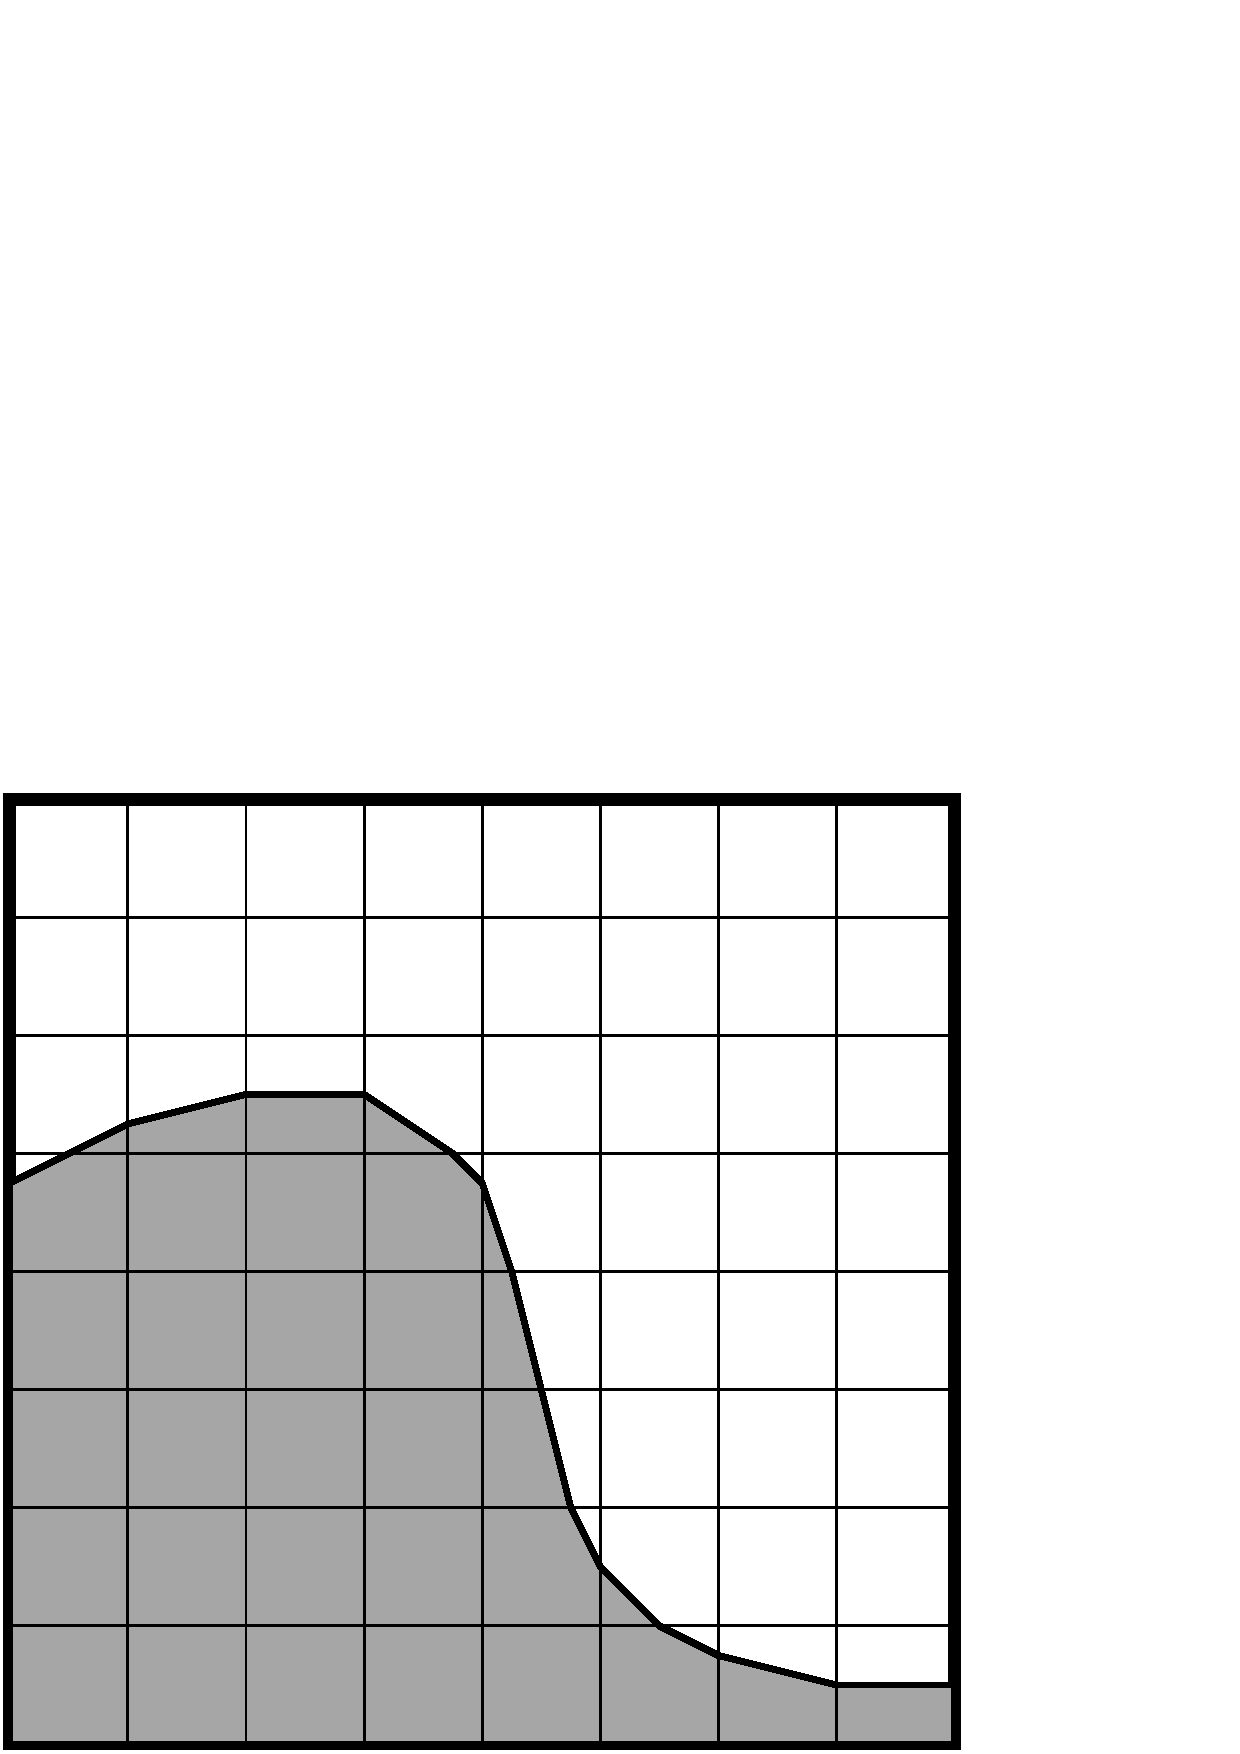
\includegraphics[width=0.25\textwidth]{./EB/EB_example.pdf}
  \caption{\label{fig::ebexample}In the embedded boundary approach to
    discretizing PDEs, the (uniform) rectangular mesh is cut by the
    irregular shape of the computational domain.  The cells in the
    mesh are label as regular, cut or covered.}
\end{figure}
Because this is a relatively simple grid
generation technique, computational meshes for rather complex geometries
can be generated quickly and robustly.  However, the technique 
can produce arbitrarily small cut cells in the domain.  In practice such small
cells can have significant impact on the robustness and stability of
traditional finite volume methods.  In this chapter we overview
a class of approaches to deal with this ``small cell'' problem in a
robust and efficient way, and discuss the tools and data that $\tt{AMReX}$
provides in order to implement them.  

Note that in a completely general implementation of the EB approach, 
there would be no restrictions on the shape or complexity of the EB surface.  
With this generality comes the possibility that the process of "cutting" the cells
results in a single $(i,j,k$) cell being broken into multiple cell fragments.
%In the block-structured context of $\tt{AMReX}$, this would trigger a significant complication
%because the state data (as well as the geometrical and cell
%connectivity information) can no longer be managed using the logically rectangular
%data structures with implied connectivity graphs that are native to the framework.  Because of this,
The current release of $\tt{AMReX}$ does not support multi-valued cells, thus there is a
practical restriction on the complexity of domains (and numerical algorithms) supported.  
AMReX support for EB with AMR will be available by early 2018;
EB support for multi-valued cells will follow.
%as it leads to complexities in data communication patterns
%and inter-level data transfer operations.  
%In both cases however, extended support is
%planned for future releases of the library, and the software infrastructure
%underlying the implementation described in this document have been designed with these
%extensions in mind.

This chapter discusses the EB tools, data structures and algorithms currently supported by
$\tt{AMReX}$ to enable the construction of discretizations of conservation law systems.
The discussion will focus on general requirements associated with building fluxes and
taking divergences of them to advance such systems.  We also give examples of how to
initialize the geometry data structures and access them to build the numerical difference
operators.

\subsection{Finite Volume Discretizations}
Consider a system of PDEs to advance a conserved quantity $U$
with fluxes $F$:
\begin{equation}
\frac{\partial U}{\partial t} + \nabla \cdot F = 0.
\label{eqn::hypsys}
\end{equation}
A conservative, finite volume discretization starts with
the divergence theorm
$$
\int_V \nabla \cdot F dV = \int_{\partial V} F \cdot n dA.
$$
In an embedded boundary cell, the ``conservative divergence'' is discretized  (as
$D^c(F)$) as follows
\begin{equation}
D^c(F) = \frac{1}{\kappa h} \left( \sum^D_{d = 1}
  (F_{d, hi}A_{d,hi} - F_{d, lo}A_{d,lo})  + F^{EB} A^{EB} \right).
\label{eqn::ebdiv}
\end{equation}

Geometry is discretely represented by volumes ($V = \kappa h^d$) and apertures 
($A= \alpha h^{d-1}$), where $h$ is the (uniform) mesh spacing at that AMR level,
$\kappa$ is the volume fraction and $\alpha$ are the area fractions.
Without multivalued cells the volume fractions, area fractions and cell and face centroids 
(see Figure~\ref{fig::volume}) are the only geometric information needed to 
compute second-order fluxes centered at the face centroids,  
and to infer the connectivity of the cells.  
Cells are connected if adjacent on the Cartesian mesh, and only via
coordinate-aligned faces on the mesh.  If an aperture, $\alpha = 0$, between two
cells, they are not directly connected to each other.

\begin{figure}[h]
  \centering
  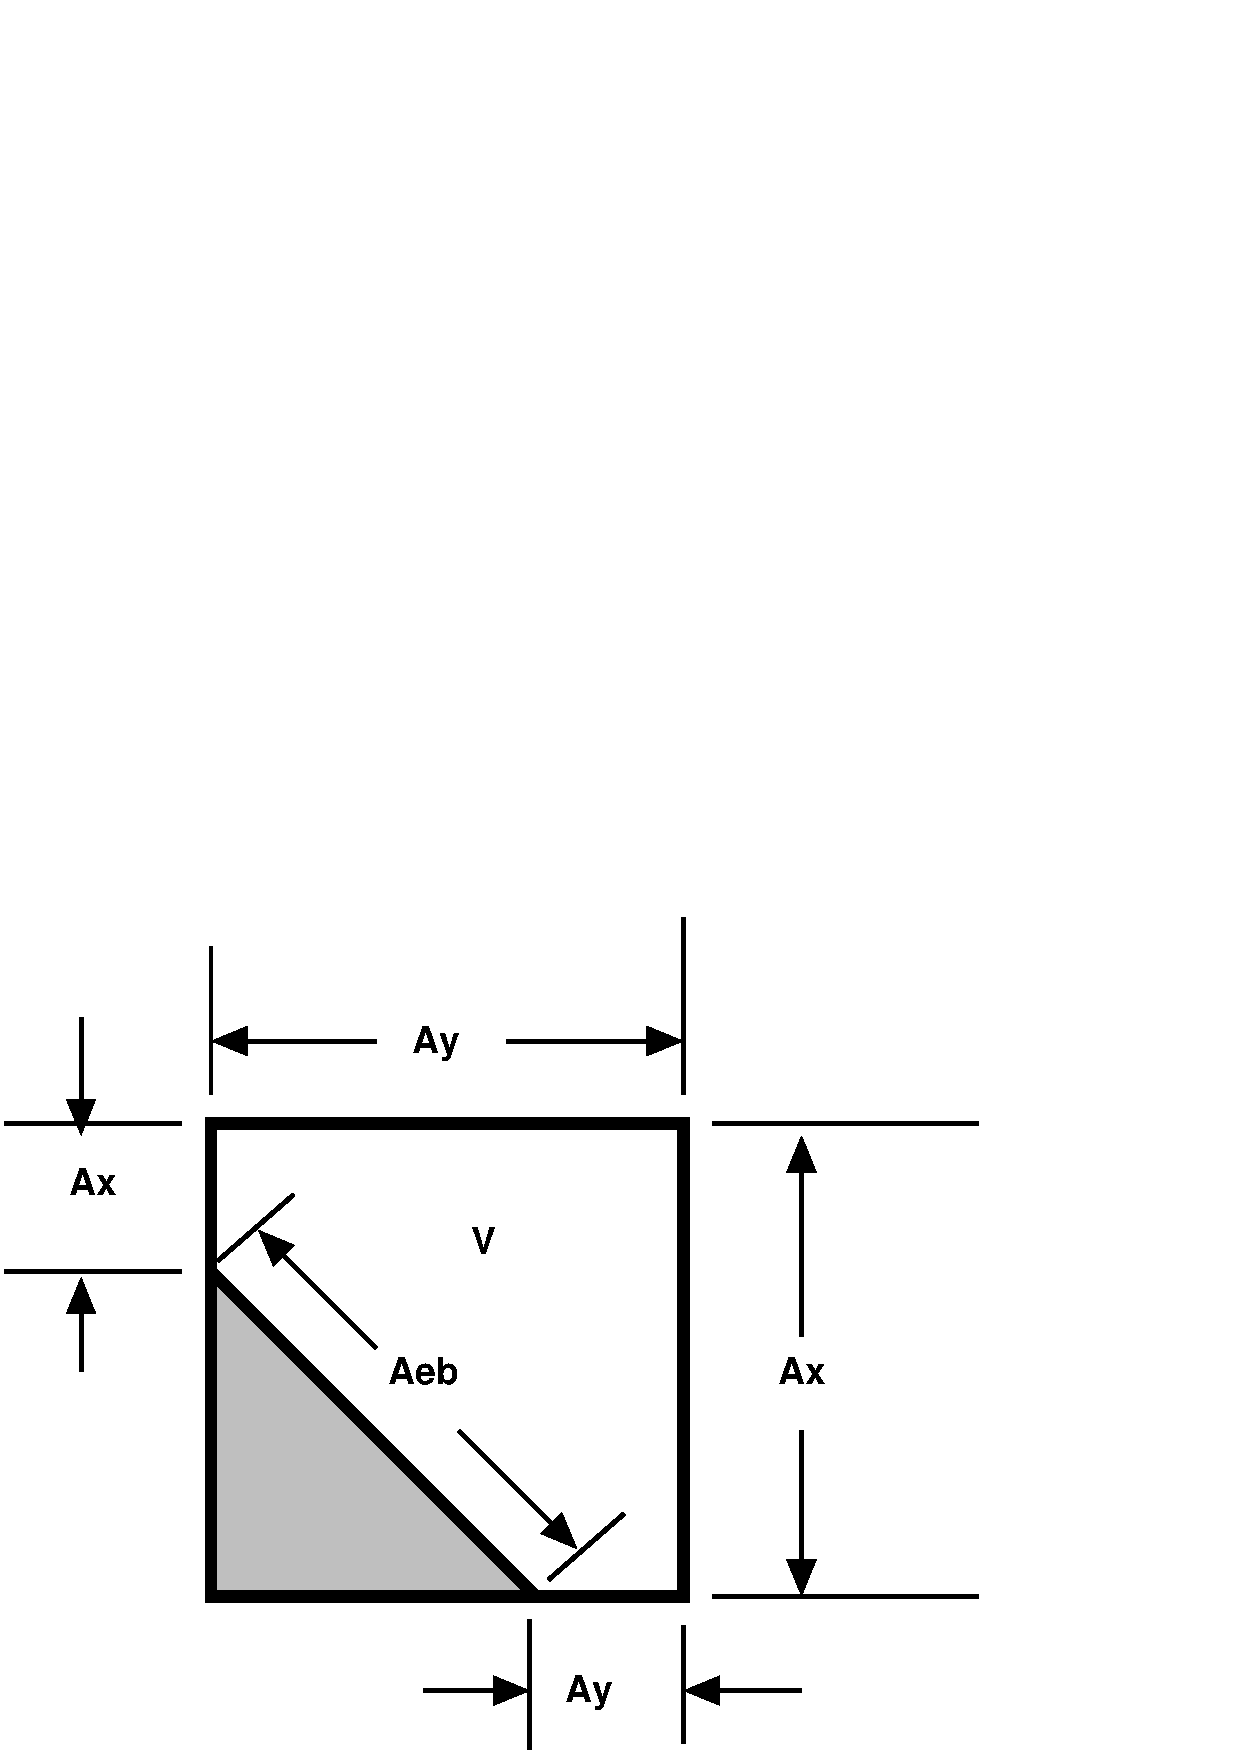
\includegraphics[width=0.25\textwidth]{./EB/areas_and_volumes.pdf}
  \hspace{1in} 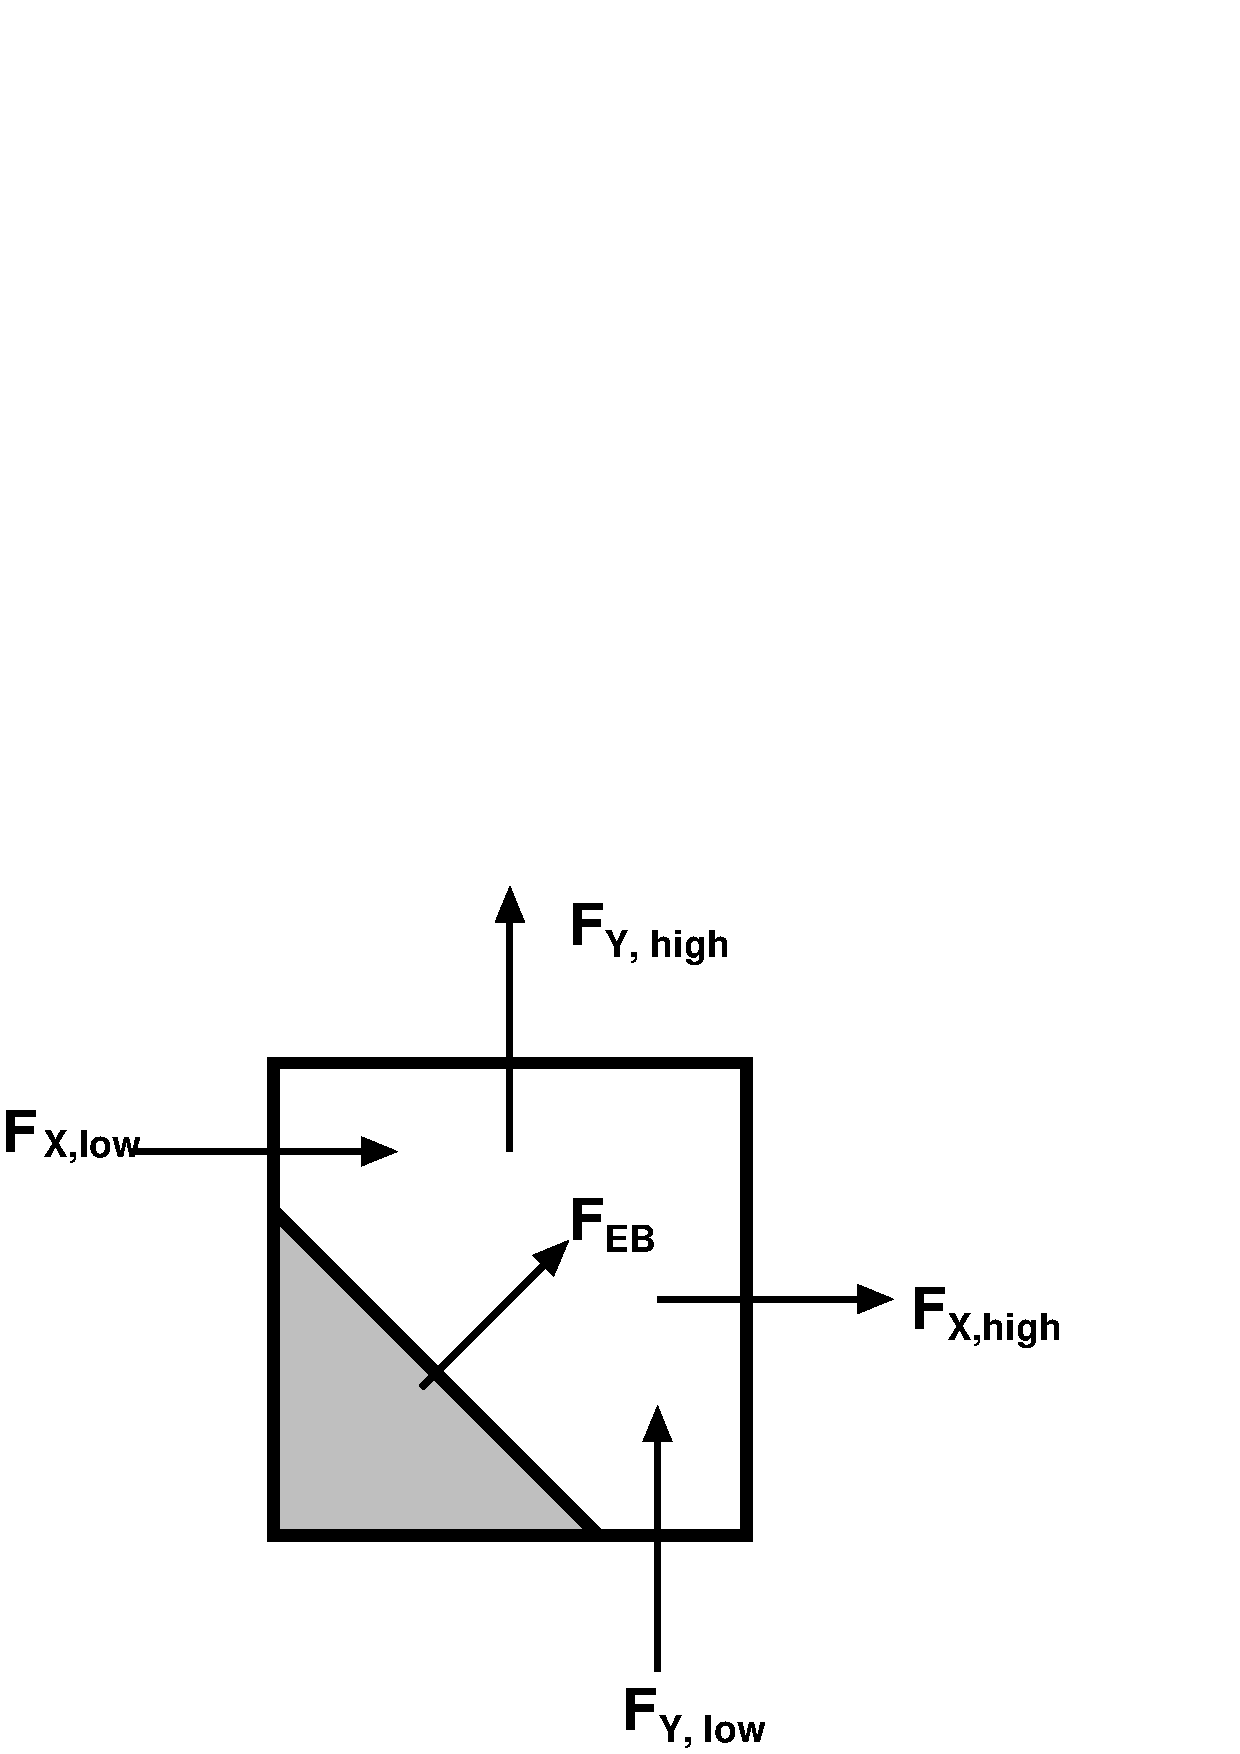
\includegraphics[width=0.25\textwidth]{./EB/eb_fluxes.pdf}
  \caption{\label{fig::volume} (a) A typical two-dimensional uniform cell that is cut by the embedded
    boundary. The grey area represents the region excluded from the calculation.   The
    portion of the cell faces (labelled with A) through which fluxes flow are the ``uncovered''
    regions of the full cell faces.  The volume (labelled V) is the uncovered
    region of the interior. (b) Fluxes in a cut cell.}
\end{figure}
%\begin{figure}[h]
%  \centering
%  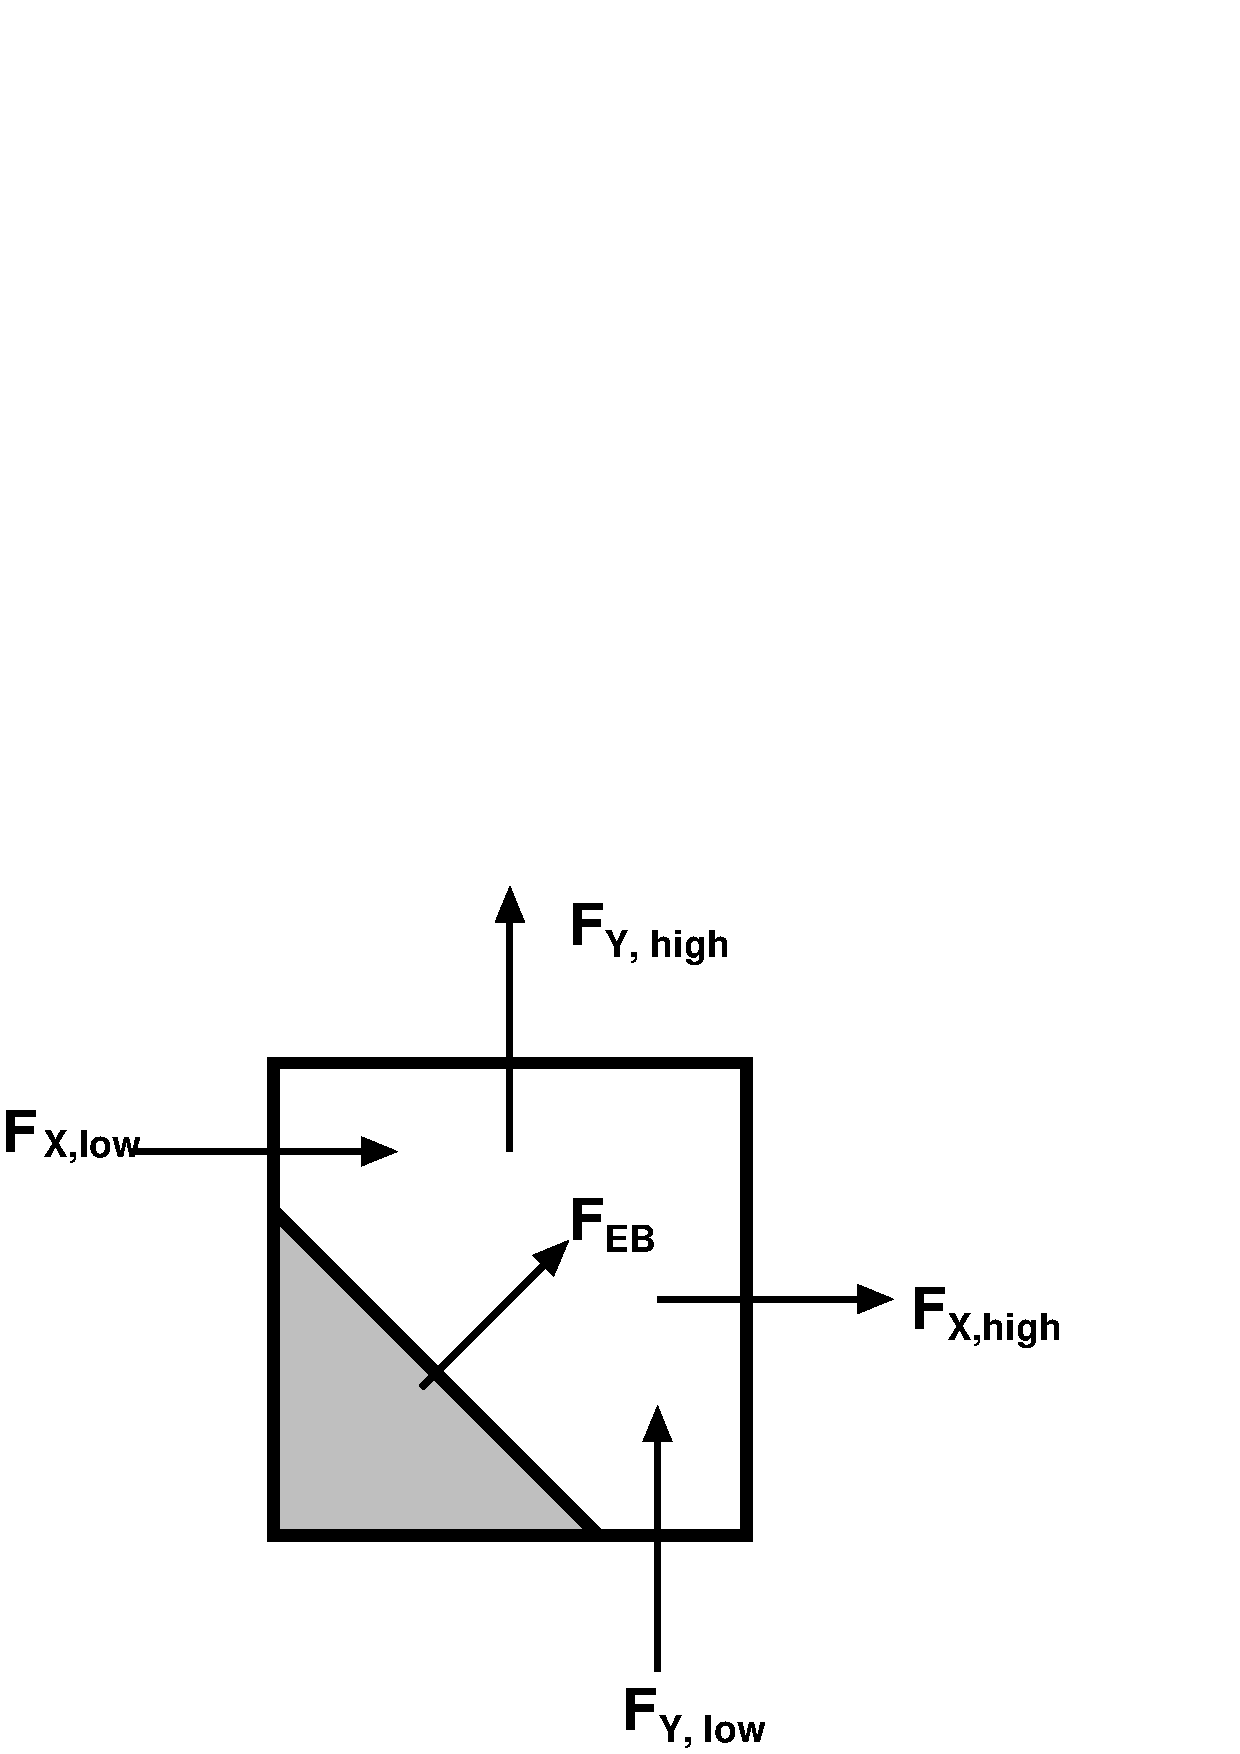
\includegraphics[width=0.25\textwidth]{./EB/eb_fluxes.pdf}
%  \caption{\label{fig::eb_fluxes}The divergence of fluxes in a cut cell.}
%\end{figure}
%\begin{itemize}
%\item
%Volume fractions,
%\item
%Area fractions,
%\item 
%Cell and face centroids
%\end{itemize}

\subsection{Small Cells And Stability}

In the context of time-explicit advance methods for, say hyperbolic conservation laws, 
a naive discretization in time of \ref{eqn::hypsys} using \ref{eqn::ebdiv},
$$
U^{n+1} = U^{n} - \delta t D^c(F)
$$
would have a time step constraint $\dt \sim h \kappa^{1/D}/V_m$,  which
goes to zero as the size of the 
smallest volume fraction $\kappa$ in the calculation.  Since EB volume fractions can
be arbitrarily small, this is an unacceptable constraint.  One way to remedy
this is to create ``non-conservative'' approximation to the divergence
$D^{nc}$, which at a cell $\ibold$, can be formed as an average of the conservative
divergences in the neighborhodd, $N_\ibold$, of $\ibold$.
$$
D^{nc}(F)_\ibold = \frac{\sum_{\jbold \in N_\ibold}\kappa_\jbold D(F)_\jbold}{\sum_{\jbold \in N_\ibold}\kappa_\jbold}
$$
Incorporating this form, the solution can be updated using a {\it hybrid divergence},
$D^H(F) = \kappa D^c(F) + (1-\kappa)D^{nc}$:
$$
U^{n+1,*} = U^n - \delta t D^H(F)
$$
However, we would like our finite-volume scheme to strictly conserve the field quantities
over the domain.  To enforce this, we calculate $\delta M$, the mass gained or
lost by not using $D^c$ directly,
$$
\delta M_\ibold = \kappa (1-\kappa)(D^c(F)_\ibold - D^{nc}(F)_\ibold)
$$
This ``excess material'' (mass, if $U=\rho$) can be {\em redistributed}\ in a time-explicit fashion
to neighboring cells, $\jbold \in N_\ibold$:
$$
\delta M_\ibold = \sum_{\jbold \in N_\ibold} \delta M_{\jbold, \ibold}.
$$
in order to preserve strict conservation over $N_\ibold$.

Note that the physics at hand may impact the optimal choice of precisely how the excess mass is distributed
in this fashion.  We introduce a weighting for redistribution, $W$,
\begin{equation}
\delta M_{\jbold, \ibold} =  \frac{\delta M_\ibold \kappa_\jbold
  W_\jbold}{\sum_{\kbold \in N_\ibold} \kappa_\kbold W_\kbold}
\label{eqn::massweight}
\end{equation}
For all $\jbold \in N_\ibold$,
$$
U^{n+1}_\jbold = U^{n+1,*}_\jbold + 
 \frac{\delta M_\ibold
  W_\jbold}{\sum_{\kbold \in N_\ibold} \kappa_\kbold W_\kbold}.
$$
 Typically, the redistribution neighborhood for each cell is one that can be reached via a monotonic
 path in each coordinate direction of unit length
(see, e.g., Figure~\ref{fig::redistribution})
\begin{figure}[h]
  \centering
  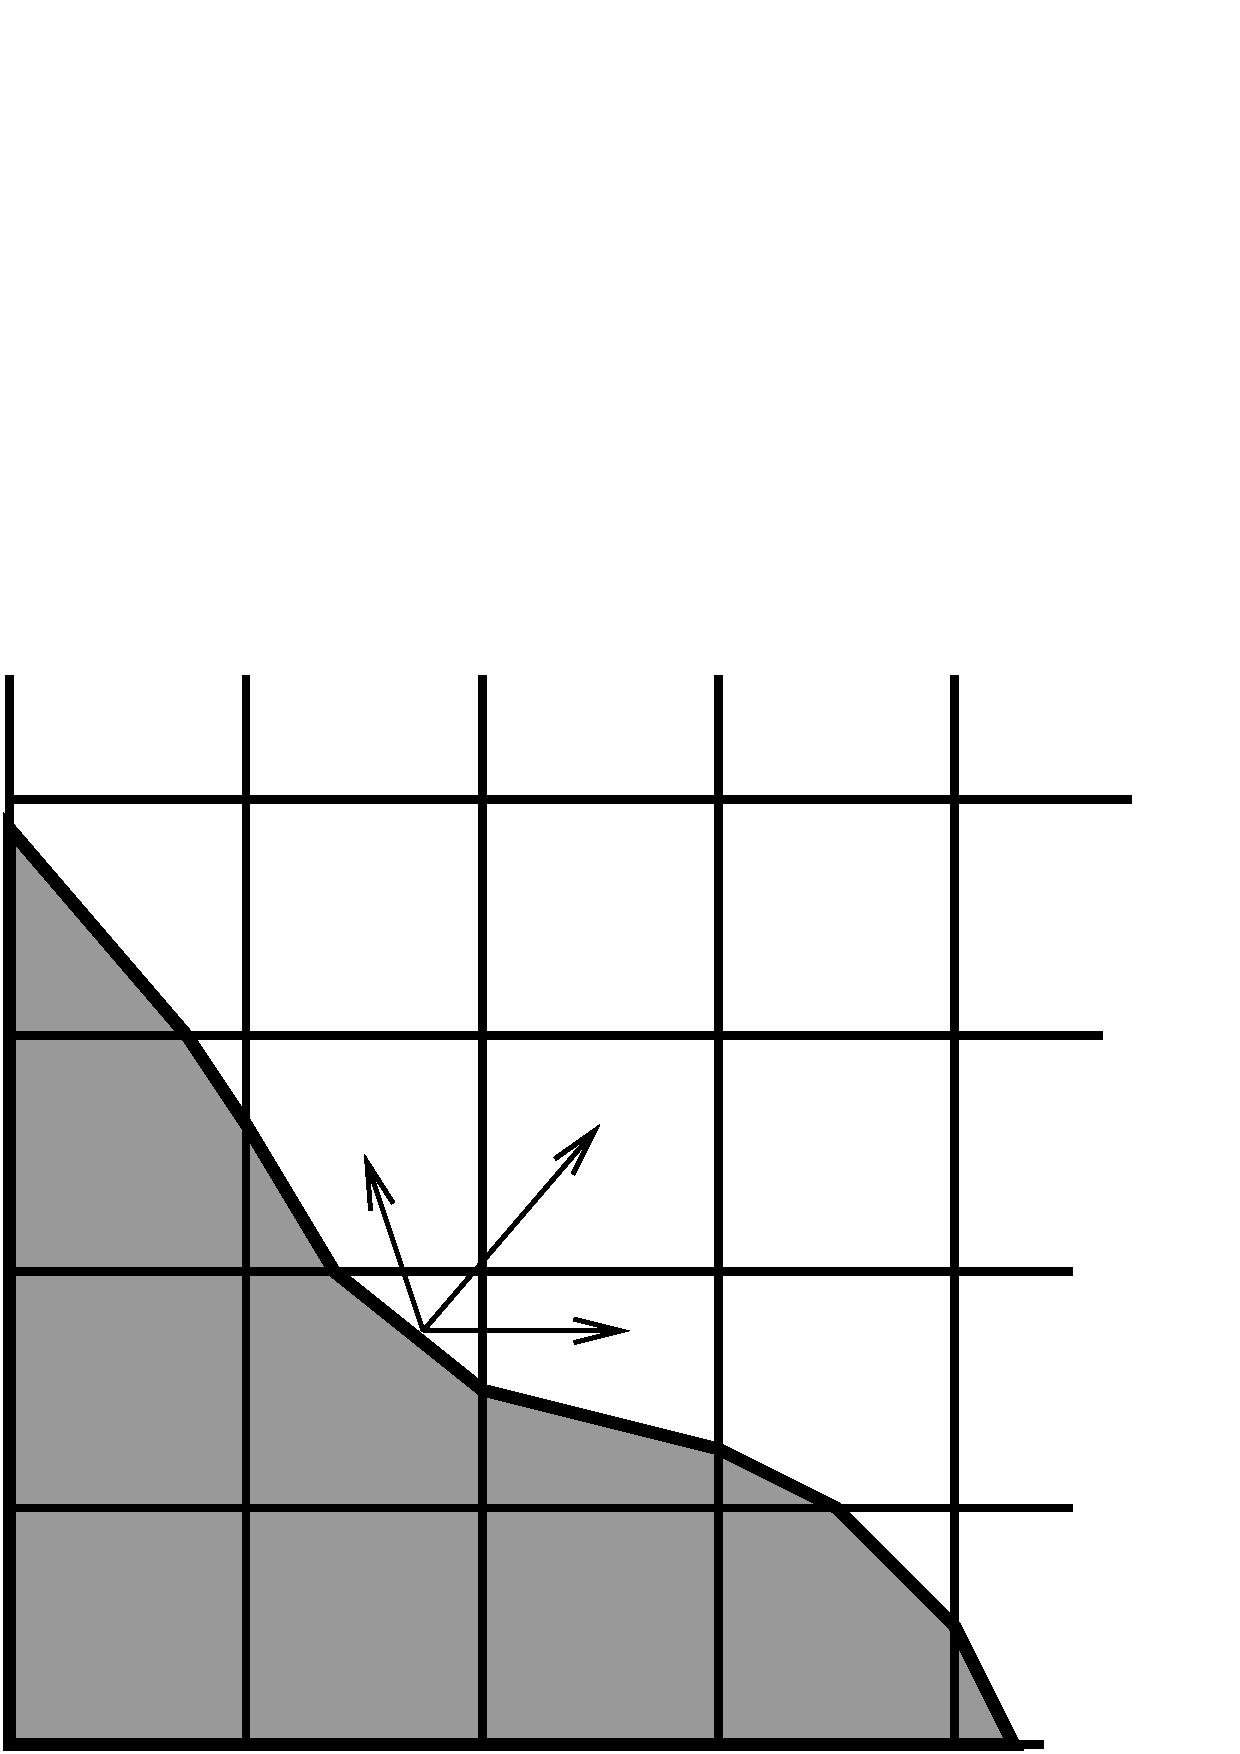
\includegraphics[width=0.25\textwidth]{./EB/redist.pdf}
\caption{\label{fig::redistribution}
Redistribution illustration.  Excess mass due to using a hybrid
divergence $D^H$ instead of the conservative divergence $D^C$ is
distributed to neighbor cells.}
\end{figure}

\section{Initializing \ebis, the Geometric Database}
\label{sec:EB:ebinit}

In $\tt{AMReX}$ the geometric information is stored in a distributed database class, \ebis, which must be
initialized at the start of the calculation.  The procedure for this
goes as follows:
\begin{itemize}
\item Define function of position which describes the surface 
      and use it define a \geom\ object (see \S
      \ref{sec:EB:geometryshop}) -- specifically, the scalar value returned by this function takes on a
      negative value inside the fluid, a positive value in the body, and identically zero at the EB.
\item Construct an \ebis\ with the \geom\ object.   This
  will fill the underlying database of geometric information, specifically tailored to the
  actual meshes that will be used.  Thus, the construction requires one to specify
  the actual mesh resolution that will be used in a calculation.
\end{itemize}

To facilitate the first step, $\tt{AMReX}$ defines a virtual class, an ``implicit function'', \baseif, which encapsulates this functionality.
An instance of a \baseif\ object is required for the construction of a \geom\ object.
\begin{lstlisting}[language=cpp]
    GeometryShop(const BaseIF& a_localGeom)
\end{lstlisting}
Although the user is free to define their own instance of this class, $\tt{AMReX}$ provides a number of preconfigured useful ones.  This
are listed in the next section.

\subsection{Example: Spherical EB}
The spherical implicit function, \sphereif, derives from \baseif, and defines the function
$$
S(\xbold) = x^2 + y^2 + z^2 - R^2,
$$
In this case, the solution domain is defined as the interior of a sphere of radius $R$.
If the sign of $S$ is reversed, the solution domain is the exterior of the sphere.
The following example illustrates how to use the \sphereif\ class to define a \geom\ object:

\begin{lstlisting}[language=cpp]

  int nx = 1024;
  Box domain(IntVect::Zero, (nx-1)*IntVect::Unit);
  Real dx = 1.0/nx;
  Real radius = 0.1;
  Real center = 0.5*RealVect::Unit;
  bool insideRegular = false;
  //this is the implicit function
  SphereIF sphere(radius, center, insideRegular);

  //this is worker object that creates geometric information given an IF
  GeometryShop workshop(sideImpMultisphere)

  //this is the global, distributed database being initialized
  EBIndexSpace*  ebis = AMReX_EBIS::instance()
  ebis->define(domain, RealVect::Zero, dx, workshop);

\end{lstlisting}

In this case, we construct an $r=0.1$ sphere, centered within a unit cube.  The mesh resolution is $1024^3$.
The \geom\ object based on this sphere is then used to construct the \ebis, as shown.

\subsubsection{Other basic shapes:}

\begin{itemize}

\item Planes are made using the class $\tt{PlaneIF}$ which given a normal
$\nbold$  and a center $\cbold$ gives the implicit function 
$$
I(\xbold) = \sum_{1<=d<=D} n_d (x_d - c_d).
$$

\begin{lstlisting}[language=cpp]
RealVect normal; 
RealVect center;
...fill in values for n and c...

PlaneIF plane(normal,point, true);
GeometryShop workshop(plane)

EBIndexSpace*  ebis = AMReX_EBIS::instance()
ebis->define(domain, RealVect::Zero, dx, workshop);

\end{lstlisting}

\item Polynomials of any form can be made using the class
  $\tt{PolynomialIF}$.  Here is an example that makes a parabola of
  the form $I(\xbold) = x - y^2 - z^2$. 
\begin{lstlisting}[language=cpp]

Vector<PolyTerm> poly;
PolyTerm mono;
Real coef;
IntVect powers;
Real amplitude = 1;
// y^2 term
coef = amplitude;
powers = IntVect::Zero;
powers[1] = 2;

mono.coef   = coef;
mono.powers = powers;
poly.push_back(mono);

// z^2 term
coef = amplitude;
            RealVect translation;
      
            for(int idir = 0; idir < SpaceDim; idir++)
            {
              int finesize = finest_domain.size()[idir];
              translation[idir] = 0.5*finesize*fine_dx;
            }
            translation[0] = 0;

            TransformIF implicit(mirror);
            implicit.translate(translation);
            impfunc.reset(implicit.newImplicitFunction());

powers = IntVect::Zero;
powers[2] = 2;
mono.coef   = coef;
mono.powers = powers;
poly.push_back(mono);

// x term
coef = -1.0;
powers = IntVect::Zero;
powers[0] = 1;
mono.coef   = coef;
mono.powers = powers;

poly.push_back(mono);

PolynomialIF mirror(poly,false);
GeometryShop workshop(mirror)
EBIndexSpace*  ebis = AMReX_EBIS::instance()
ebis->define(domain, RealVect::Zero, dx, workshop);
\end{lstlisting}

\end{itemize}
\subsection{Implicit Function Transformation Tools}

More complex domains can be constructed by composing these fundamental shapes.
$\tt{AMReX}$ contains the following classes to compose implicit functions:
\begin{itemize}
\item $\tt{TransformIF}$    allows for translations and rotations of an implicit function.
\item $\tt{UnionIF}$        produces the union of two implicit functions.  
\item $\tt{IntersectionIF}$ produces the intersection of two implicit functions.
\item $\tt{LatheIF}$        creates a 3D implicit function as the surface of
  revolution of a 2D implicit function.
\end{itemize}

\subsection{Multi-sphere example}
The following example creates a geometry using multiple spheres:

\begin{lstlisting}[language=cpp]

vector<Real>     radius(numSpheres);
vector<RealVect> center(numSpheres);
...
//create an implicit function for each sphere
vector<BaseIF*>  spheres(numSpheres);

for(int isphere = 0; isphere < numSpheres; isphere++)
{
  // Create sphere at each origin and translate
  SphereIF sphereAtZero(radius[isphere], RealVect::Zero, false);
  TransformIF* movedSphere = new TransformIF(sphereAtZero);
  movedSphere->translate(center[isphere]);
  spheres[isphere] = static_cast<BaseIF*>(movedSphere);
}
// Create implicit function as intersection of spheres
IntersectionIF impMultisphere(spheres);

// Fluid will in the complement space outside the sphere
ComplementIF sideImpMultisphere(impMultisphere, false);

// Construct the geometryshop
GeometryShop workshop(sideImpMultisphere)
\end{lstlisting}

\subsection{Geometric example 2 -- Surface of revolution}

Here is an example that creates a geometric construction using a
surface of revolution of a set of polygons.   This particular example
only makes sense in three dimensions.   With the right polygons, it
creates the surface shown in \ref{fig::revolution}.

\begin{lstlisting}[language=cpp]

/// define EBIndexSpace from the surface of revolution of a set of polygons
void
defineGeometry(const Real& fine_dx, const  Box& finest_domain, int max_grid_size)
{
  amrex::Print() << "creating geometry from polygon surfaces of revolution" << endl;

  // These  the polygons that get built around the z axis
  Vector<Vector<RealVect> > polygons;
  //....fill the polygons any way you like//

  // Make the Array of (convex) polygons (Arrays of points) into a union
  // of convex polygons, each made from the intersection of a set of half
  // planes/spaces - all represented by implicit functions.

  // A list of all the polygons as implicit functions
  Vector<BaseIF*> polytopes;
  polytopes.resize(0);
  int numPolys = polygons.size();
  // Process each polygon
  for (int p = 0; p < numPolys; p++)
  {
    // All the half planes/spaces used to make a polygon
    Vector<BaseIF*> planes;
    planes.resize(0);

    // Get the current polygon (as a Array of points)
    const Vector<RealVect>& polygon = polygons[p];

    // Get the number of points in the polygon
    int numPts = polygon.size();

    // Process each pair of points
    for (int n = 0; n < numPts; n++)
    {
      // The normal and point is space used to specify each half plane/space
      RealVect normal(RealVect::Zero);
      RealVect point;

      // Set the normal remembering that the last point connects to the first
      // point.
      normal[0] = -(polygon[(n+1) % numPts][1] - polygon[n][1]);
      normal[1] =  (polygon[(n+1) % numPts][0] - polygon[n][0]);

      point = polygon[n];

      // Generate the appropriate half plane/space (as an implicit function)
      PlaneIF* plane;
      plane = new PlaneIF(normal,point,true);

      // Save the result
      planes.push_back(plane);
    }

    // Intersect all the half planes/spaces to create an implicit function
    // that represents the polygon
    IntersectionIF* polygonIF = new IntersectionIF(planes);

    polytopes.push_back(polygonIF);
  }

  //this makes the cross section the union of all the polgons (around
  //z-axis, recall)
  UnionIF crossSection(polytopes);
            
  // In 3D rotate about the z-axis 
  LatheIF lathe(crossSection, false);

  //we are starting around the z axis so we need to translate
  //over to the center of the x-y plane
            
  RealVect translation;
  for(int idir = 0; idir < SpaceDim; idir++)
  {
    translation[idir] = 0.5*finest_domain.size()[idir]*fine_dx;
  }
  translation[2] = 0;
  TransformIF implicit(lathe);
  implicit.translate(translation);

  //create a workshop from translated surface of revolution
  GeometryShop gshop(implicit, false);
  //define th geometric database
  AMReX_EBIS::instance()->define(finest_domain, RealVect::Zero,
                                 fine_dx, gshop, max_grid_size);
}

\end{lstlisting}

\begin{figure}[h]
  \centering
  \includegraphics[width=0.375\textwidth]{./EB/revolution.pdf}
  \caption{\label{fig::revolution} Zero surface of an implicit
    function made using a surface of revolution.}
\end{figure}
\subsection{Geometric example 3 -- A Sphere Inside a Parabola}

Here is an example that creates a geometry of a sphere contained
within a parabola. This code
creates the surface shown in \ref{fig::parabolasphere}.

\begin{lstlisting}[language=cpp]
Vector<PolyTerm> poly;

PolyTerm mono;
Real coef;
IntVect powers;
Real amplitude = 1;

// y^2 term
coef = amplitude;
powers = IntVect::Zero;
powers[1] = 2;

mono.coef   = coef;
mono.powers = powers;

poly.push_back(mono);

// z^2 term
coef = amplitude;
powers = IntVect::Zero;
powers[2] = 2;
mono.coef   = coef;
mono.powers = powers;
poly.push_back(mono);

// x term
coef = -1.0;
powers = IntVect::Zero;
powers[0] = 1;
mono.coef   = coef;
mono.powers = powers;

poly.push_back(mono);

PolynomialIF mirror(poly,false);
RealVect translation;

for(int idir = 0; idir < SpaceDim; idir++)
{
  int finesize = finest_domain.size()[idir];
  translation[idir] = 0.5*finesize*fine_dx;
}
RealVect center = translation;
translation[0] = 0;

TransformIF transform(mirror);
transform.translate(translation);

Real radius = 0.2*center[0];
SphereIF sphere(radius, center, true);
Vector<BaseIF*> funcs(2);
funcs[0] = &transform;
funcs[1] = &sphere;
UnionIF implicit(funcs);
impfunc.reset(implicit.newImplicitFunction());
GeometryShop gshop(impfunc, false);
//define th geometric database
AMReX_EBIS::instance()->define(finest_domain, RealVect::Zero,
                                 fine_dx, gshop, max_grid_size);
\end{lstlisting}

\begin{figure}[h]
  \centering
  \includegraphics[width=0.375\textwidth]{./EB/parabsphere.pdf}
  \caption{\label{fig::parabolasphere} Zero surface of an implicit
    function made the above code.}
\end{figure}

\section{$\tt{EBFarrayBox}$}

The fundamental data structure for embedded boundary calculations is 
$\tt{EBFArrayBox}$. $\tt{EBFArrayBox}$ is an a $\tt{FArrayBox}$ with two extra
data members.
\begin{itemize}
\item $\tt{EBFArrayBox::getEBISBox}$ returns an $\tt{EBISBox}$, a data
  structure that contains the geometric information of an \ebis\ but
  restricted to a given box.
\item $\tt{EBFArrayBox::getEBCellFlagFab}$  is a
  $\tt{BaseFab<EBCellFlag>}$, where $\tt{EBCellFlag}$ is a class which
  is a class with tools that compactly specifies local cell connectivities
  on a box.
\end{itemize}
If one compiles with $\tt{AMREX\_USE\_EB = TRUE}$, the state data managed by
the ${\tt Amr}$ class is automatically of type $\tt{EBFArrayBox}$ (typically the data
is exposed explicitly as a $\tt{MultiFab}$, but the additional functionality
may be accessed through a C++ type cast. The
$\tt{EBCellFlagFab}$ can be used down in $\tt{Fortran}$, e.g., to choose
locally whether EB-specific operations and data are required for constructing
discretizations.  In the next section, we show examples of this workflow.

\subsection{$\tt{EBFarrayBox}$ Usage Example}
In order to make these EB concepts more concrete, we discuss here sample code
that appears in the $\tt{AMReX}$ tutorial, $\tt{Tutorial/EB/CNS}$.  This code
implements a time-explicit second-order method of lines integrator for hyperbolic
and parabolic transport based on a gamma-law gas EOS and constant transport
properties.  This example also demonstrates how to avoid the more complex/expensive
EB-related logic if the tile under consideration has no cut cells.

\begin{lstlisting}[language=cpp]
void
CNS::compute_dSdt (const MultiFab& S, MultiFab& dSdt, Real dt,
                   EBFluxRegister* fr_as_crse, EBFluxRegister* fr_as_fine)
{
    BL_PROFILE("CNS::compute_dSdt()");

    const Real* dx = geom.CellSize();
    const int ncomp = dSdt.nComp();

#ifdef _OPENMP
#pragma omp parallel
#endif
     {
        //fluxes for the advance
        std::array<FArrayBox,AMREX_SPACEDIM> flux;

        for (MFIter mfi(S, MFItInfo().EnableTiling(hydro_tile_size).SetDynamic(true));
                        mfi.isValid(); ++mfi)
        {
            //this tile is the subset of the box over which we are computing
            const Box& bx = mfi.tilebox();

            //because we have compiled with AMREX_USE=EB_TRUE, the
            //MultiFab holds EBFArrayBox(es) so we can do this cast
            const EBFArrayBox& sfab
                = dynamic_cast<EBFArrayBox const&>(S[mfi]);
            
            //here we are getting the collection of flags so we know
            //kind of grid this is and if it is an EB grid, we have
            //the connectivity info
            const EBCellFlafgFab & flag = sfab.getEBCellFlagFab();

            if (flag.getType(bx) == FabType::covered) 
            {
              //this tile is covered so there are no meaningful data here
                dSdt[mfi].setVal(0.0, bx, 0, ncomp);
            } 
            else 
            {
              //create the flux holders for this tile
              for (int idim=0; idim < AMREX_SPACEDIM; ++idim) 
              {
                flux[idim].resize(amrex::surroundingNodes(bx,idim),ncomp);
              }

              if (flag.getType(amrex::grow(bx,1)) == FabType::regular)
              {
                //this tile has no cut cells so we can just proceed
                //with a (cheaper) non-eb call

                cns_compute_dudt(BL_TO_FORTRAN_BOX(bx),
                BL_TO_FORTRAN_ANYD(dSdt[mfi]),
                BL_TO_FORTRAN_ANYD(S[mfi]),
                BL_TO_FORTRAN_ANYD(flux[0]),
                BL_TO_FORTRAN_ANYD(flux[1]),
                BL_TO_FORTRAN_ANYD(flux[2]),
                dx, &dt);

              }
              else
              {
                //this tile has cut cells so we have to send into Fortran
                //EBCellFlagFAB as well as lots of geometric
                //information
                //the areafrac and facecent objects are member data
                //filled using EBISBox
                cns_eb_compute_dudt(BL_TO_FORTRAN_BOX(bx),
                BL_TO_FORTRAN_ANYD(dSdt[mfi]),
                BL_TO_FORTRAN_ANYD(S[mfi]),
                BL_TO_FORTRAN_ANYD(flux[0]),
                BL_TO_FORTRAN_ANYD(flux[1]),
                BL_TO_FORTRAN_ANYD(flux[2]),
                BL_TO_FORTRAN_ANYD(flag),
                BL_TO_FORTRAN_ANYD(volfrac[mfi]),
                BL_TO_FORTRAN_ANYD(bndrycent[mfi]),
                BL_TO_FORTRAN_ANYD(areafrac[0][mfi]),
                BL_TO_FORTRAN_ANYD(areafrac[1][mfi]),
                BL_TO_FORTRAN_ANYD(areafrac[2][mfi]),
                BL_TO_FORTRAN_ANYD(facecent[0][mfi]),
                BL_TO_FORTRAN_ANYD(facecent[1][mfi]),
                BL_TO_FORTRAN_ANYD(facecent[2][mfi]),
                dx, &dt);
              }
            }
          }
        }

\end{lstlisting}

This is the main loop in the routine to advance the state.  The state, $\tt{S}$, comes into this routine with grow cells
properly filled, and this routine features a $\tt{MultiFab}$ iterator loop to step through this data, tile-by-tile and compute
$\tt{dSdt}$.  Here, we see that the definition of $\tt{sfab}$ incorporates the aforementioned type cast, enabling queries about
the EB nature of the data.  Of the two possiblities handled, the ``regular'' type without cut cells has a much simpler interface.
The EB version takes all the same data, but additionally requires (dense) data to specify the volume and face area fractions,
centroid information, and the $\tt{flag}$ structure that will be queried pointwise for the local cell connectivity.

\subsection{Fortran code Snippets}
Much of the code to compute these fluxes and their divergence in this example is too detailed to step through in this context.
There are however a few salient features worth pointing out.

\subsubsection{The data is cell-centered, even cut cells}
In order to simplify the construction second-order discretizations, we can base all the numerical operations on the assumption
that all cell-based data lives at the center of the {\em full}\ cell containing the cut cells.  This means that when we take a
standard centered difference between cell data at $(i,j,k)$ and $(i+1,j,k)$, e.g., we get a gradient value that is second-order and
centered on the full face at $i+1/2$, regardless of the aperature.

\subsubsection{Many EB operations can be organized as post-processing}
Recall that a second-order finite-volume scheme requires that fluxes
be centered on the face {\em centroid}.  This can be accomplished by post-processing face-centered fluxes with a linear interpolation
of adjacent face values.  The resulting centroid-based fluxes are second-order, and can be used to construct the conservative
divergence we seek.  Note that this operation requires the location of the face centroids, and increases the grow cell requirement
of the flux operators, as does the necessity to form the {\em hybrid divergence}\ operator discussed above.

\subsubsection{The $\tt{flag}$ data}
$\tt{AMReX}$ provides functions that query the $\tt{flag}$ data in order to infer the local connectivity of cells.  For example,
the cell itself or its neighbors may be covered or cut.  If cut, the data is centered at the center of the full cell.  If covered,
the data is invalid and should not be involved in the fluid advance.  An example of such a call is:

\begin{lstlisting}[language=Fortran]
   call get_neighbor_cells(cellflag(i,j,k),nbr)
\end{lstlisting}

Here, for the $\tt{flag}$ at $(i,j,k)$ is used to fill a local $3^3$ array of integers with the value $1$ if connected to $(i,j,k)$,
and $0$ if not.  Similar queries:

\begin{lstlisting}[language=Fortran]
   is_covered_cell(cellflag(i,j,k))
   is_single_valued_cell(cellflag(i,j,k)
\end{lstlisting}
can be used to gather additional detail.

Below, we show a partial listing of the $\tt{cns_eb_compute_dudt}$ code, specifically after the face-centered fluxes have been computed,
and showing part of the work necessary to interpolate them to face centroids (while appropriately handling covered data).

\begin{lstlisting}[language=Fortran]
    do n = 1, ncomp

       !
       ! First, we compute conservative divergence on (lo-2,hi+2)
       !
       iwall = 0
       do       k = lo(3)-2, hi(3)+2
          do    j = lo(2)-2, hi(2)+2
             do i = lo(1)-2, hi(1)+2
                divc(i,j,k) = (fluxx(i,j,k,n)-fluxx(i+1,j,k,n))*dxinv(1) &
                     +        (fluxy(i,j,k,n)-fluxy(i,j+1,k,n))*dxinv(2) &
                     +        (fluxz(i,j,k,n)-fluxz(i,j,k+1,n))*dxinv(3)
             end do

             do i = lo(1)-2, hi(1)+2
                if (is_covered_cell(cellflag(i,j,k))) then
                   divc(i,j,k) = 0.d0
                else if (is_single_valued_cell(cellflag(i,j,k))) then

                   call get_neighbor_cells(cellflag(i,j,k),nbr)

                   ! x-direction lo face
                   if (apx(i,j,k).lt.1.d0) then
                      if (centx_y(i,j,k).le.0.d0) then
                         fracy = -centx_y(i,j,k)*nbr(0,-1,0)
                         if(centx_z(i,j,k).le. 0.0d0)then
                            fracz = - centx_z(i,j,k)*nbr(0,0,-1)
                            fxm = (1.d0-fracz)*(     fracy *fluxx(i,j-1,k  ,n)  + &
                                 &             (1.d0-fracy)*fluxx(i,j  ,k  ,n)) + &
                                 &      fracz *(     fracy *fluxx(i,j-1,k-1,n)  + &
                                 &             (1.d0-fracy)*fluxx(i,j  ,k-1,n))
                         else
                            fracz =  centx_z(i,j,k)*nbr(0,0,1)
                            fxm = (1.d0-fracz)*(     fracy *fluxx(i,j-1,k  ,n)  + &
                                 &             (1.d0-fracy)*fluxx(i,j  ,k  ,n)) + &
                                 &      fracz *(     fracy *fluxx(i,j-1,k+1,n)  + &
                                 &             (1.d0-fracy)*fluxx(i,j  ,k+1,n))
                         endif
                      else
                         fracy = centx_y(i,j,k)*nbr(0,1,0)
                         if(centx_z(i,j,k).le. 0.0d0)then
                            fracz = -centx_z(i,j,k)*nbr(0,0,-1)
                            fxm = (1.d0-fracz)*(     fracy *fluxx(i,j+1,k  ,n)  + &
                                 &             (1.d0-fracy)*fluxx(i,j  ,k  ,n)) + &
                                 &      fracz *(     fracy *fluxx(i,j+1,k-1,n)  + &
                                 &             (1.d0-fracy)*fluxx(i,j  ,k-1,n))
                         else
                            fracz = centx_z(i,j,k)*nbr(0,0,1)
                            fxm = (1.d0-fracz)*(     fracy *fluxx(i,j+1,k  ,n)  + &
                                 &             (1.d0-fracy)*fluxx(i,j  ,k  ,n)) + &
                                 &      fracz *(     fracy *fluxx(i,j+1,k+1,n)  + &
                                 &             (1.d0-fracy)*fluxx(i,j  ,k+1,n))
                         endif
                      end if
                   else
                      fxm = fluxx(i,j,k,n)
                   end if

           <..... similar code for other fluxes removed ....>

                   iwall = iwall + 1
                   if (n .eq. 1) then
                      call compute_hyp_wallflux(divhyp(:,iwall), i,j,k, q(i,j,k,qrho), &
                           q(i,j,k,qu), q(i,j,k,qv), q(i,j,k,qw), q(i,j,k,qp), &
                           apx(i,j,k), apx(i+1,j,k), &
                           apy(i,j,k), apy(i,j+1,k), &
                           apz(i,j,k), apz(i,j,k+1))
                      call compute_diff_wallflux(divdiff(:,iwall), dxinv, i,j,k, &
                           q, qlo, qhi, &
                           lam, mu, xi, clo, chi, &
                           bcent, blo, bhi, &
                           apx, axlo, axhi, &
                           apy, aylo, ayhi, &
                           apz, azlo, azhi)
                   end if

                   divwn = divhyp(n,iwall) + divdiff(n,iwall)

                   ! we assume dx == dy == dz
                   divc(i,j,k) = -((apx(i+1,j,k)*fxp - apx(i,j,k)*fxm) * dxinv(1) &
                        +          (apy(i,j+1,k)*fyp - apy(i,j,k)*fym) * dxinv(2) &
                        +          (apz(i,j,k+1)*fzp - apz(i,j,k)*fzm) * dxinv(3) &
                        +          divwn * dxinv(1)) / vfrac(i,j,k)
                end if
             end do
          end do
       end do

\end{lstlisting}

One can easily identify the logic and portions of the code devoted toward the EB corrections.  Note, in particular,
that diffusive fluxes into the EB need only be computed on cut cells.

\subsubsection{There are many approaches}
The ``fixes'' that need to occur in these EB algorithms can be managed in a number of ways, depending on the
needs of the application and programming style.  In this example, the geometrical data is used to fill dense
data structures so that the sparse geometry information is available uniformally over the entire box.
Also, the cell types are queried point-by-point in order to form the appropriate stencil. Obviously then
there is a performance penalty if many of the cells in tile are not actually cut.  There is clearly a trade-off
in such designs.  Alternatively, one might build sparse data structures similar to those $\tt{AMReX}$ uses to manage
particles, and apply the EB corrections on this sparse set directly.  Future releases of $\tt{AMReX}$ will
feature an expanded set of EB tutorials to demonstrate an evolving set of tools provided.


\chapter{Visualization}\label{Chap:Visualization}
There are several visualization tools that can be used for \amrex\
plotfiles.  The standard tool used within the
\amrex-community is \amrvis, a package developed and supported 
by CCSE that is designed specifically for highly efficient visualization
of block-structured hierarchical AMR data.
Plotfiles can also be viewed using the \visit, \paraview, and \yt packages.
Particle data can be viewed using \paraview.

\section{\amrvis}

Our favorite visualization tool is \amrvis. We heartily encourage you
to build the {\tt amrvis2d} and {\tt amrvis3d} executables, and to try using them
to visualize your data. A very useful feature is View/Dataset, which
allows you to actually view the numbers in a spreadsheet that is nested
to reflect the AMR hierarchy -- this can be handy for
debugging. You can modify how many levels of data you want to see,
whether you want to see the grid boxes or not, what palette you use,
etc.  Here are some instructions and tips for using \amrvis:

\begin{enumerate}

\item Download and build \amrvis:
\begin{verbatim}
git clone https://ccse.lbl.gov/pub/Downloads/Amrvis.git
\end{verbatim}

Then {\tt cd} into {\tt Amrvis/}, edit the {\tt GNUmakefile} by
setting {\tt COMP} to the compiler suite you have.

Type {\tt make DIM=2} or {\tt make DIM=3} to build, 
resulting in an executable that looks like {\tt amrvis2d...ex}.

If you want to build amrvis with {\tt DIM=3}, you must first
download and build {\tt volpack}:
\begin{verbatim}
git clone https://ccse.lbl.gov/pub/Downloads/volpack.git
\end{verbatim}

Then {\tt cd} into {\tt volpack/} and type {\tt make}.

Note: \amrvis\ requires the OSF/Motif libraries and headers. If you don't have these 
you will need to install the development version of motif through your package manager. 
{\tt lesstif} gives some functionality and will allow you to build the amrvis executable, 
but \amrvis\ may exhibit subtle anomalies.

On most Linux distributions, the motif library is provided by the
{\tt openmotif} package, and its header files (like {\tt Xm.h}) are provided
by {\tt openmotif-devel}. If those packages are not installed, then use the
OS-specific package management tool to install them. 

You may then want to create an alias to {\tt amrvis2d}, for example
\begin{verbatim}
alias amrvis2d /tmp/Amrvis/amrvis2d...ex
\end{verbatim}

\item Run the command {\tt cp Amrvis/amrvis.defaults \textasciitilde/.amrvis.defaults}.
Then, in your copy, edit the line containing ``{\tt palette}'' line to point to, e.g., 
``{\tt palette  /home/username/Amrvis/Palette}''.  The other lines control
options such as the initial field to display, the number format, widow size, etc.
If there are multiple instances of the same option, the last option takes precedence.

\item Generally the plotfiles have the form {\tt pltXXXXX} 
  (the {\tt plt} prefix can be changed), where {\tt XXXXX} is a number 
  corresponding to the timestep the file
  was output.  {\tt amrvis2d <filename>} or {\tt amrvis3d <filename>}
  to see a single plotfile, 
  or for 2D data sets, {\tt amrvis2d -a plt*}, which will animate the 
  sequence of plotfiles.

  You can use the ``Variable'' menu to change the variable.
  You can left-click drag a box around a region
  and click "View'' $\rightarrow$ ``Dataset''
  in order to look at the actual numerical values
  (see Figure \ref{Fig:Amrvis}).
  Or you can simply left click on a point to obtain the numerical value.
  You can also export the
  pictures in several different formats under "File/Export".
  In 2D you can right and center click to get line-out plots.
  In 3D you can right and center click to change the planes, and the hold
  shift+(right or center) click to get line-out plots.

\begin{figure}[tb]
\centering
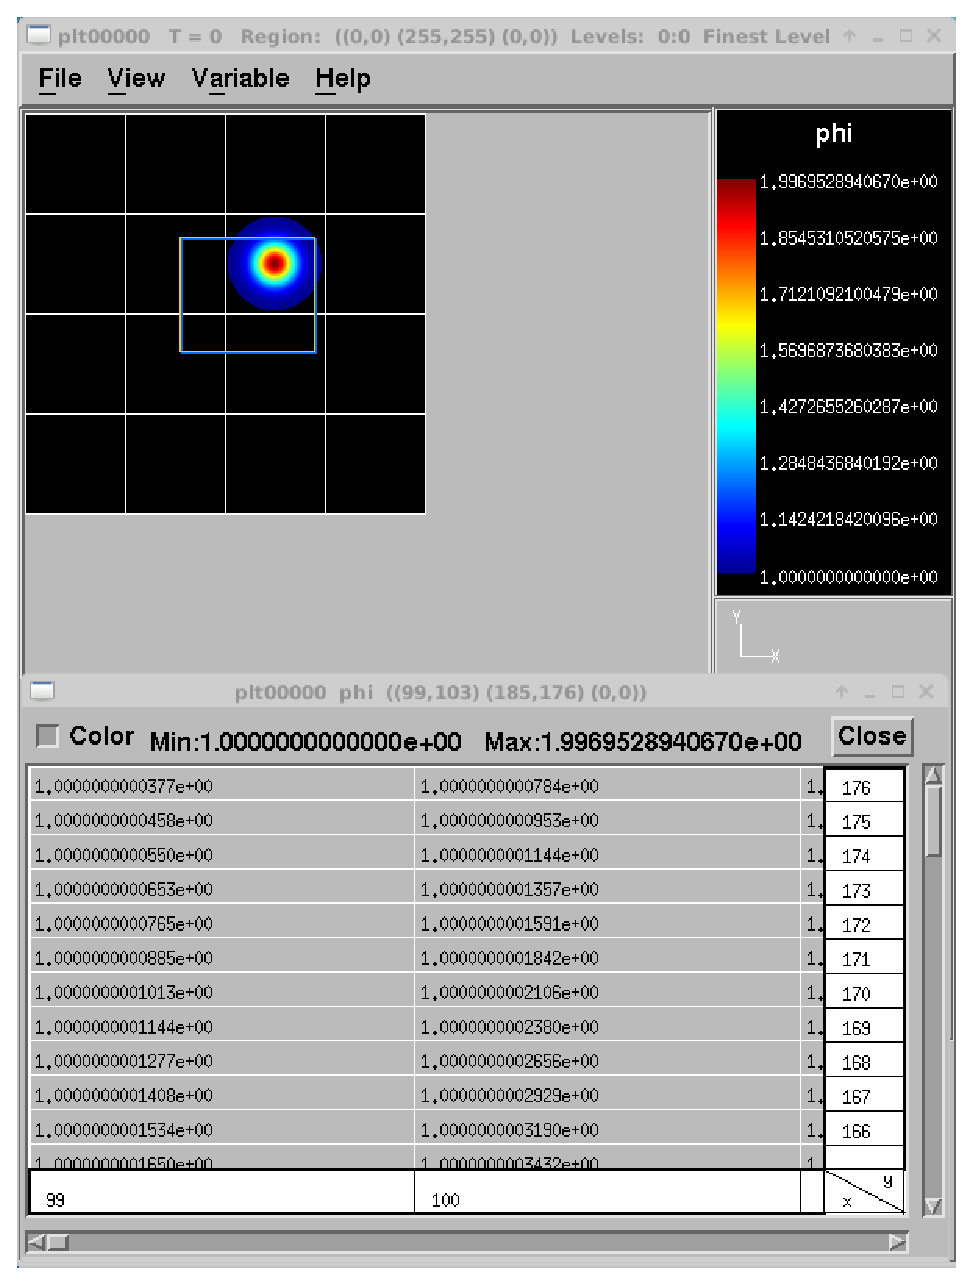
\includegraphics[width=2.5in]{./Visualization/Amrvis_2d}
~~~
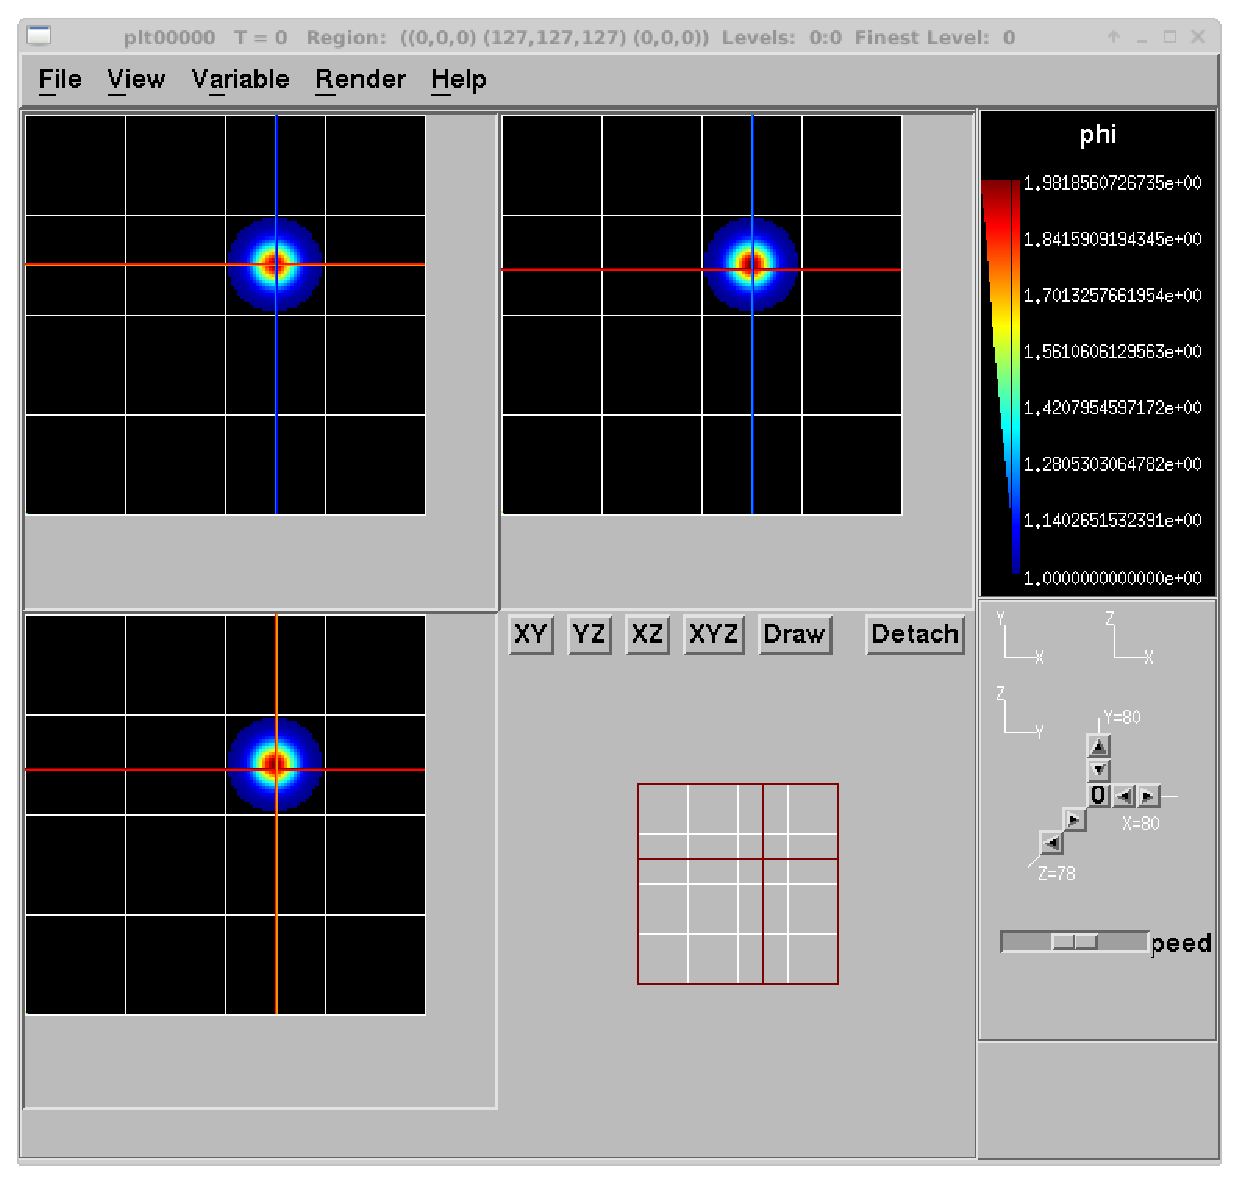
\includegraphics[width=2.5in]{./Visualization/Amrvis_3d}
\caption{2D and 3D images generated with Amrvis}
\label{Fig:Amrvis}
\end{figure}

  We have created a number of routines to convert \amrex\ plotfile data
  other formats (such as MATLAB), but in order to properly interpret 
  the hierarchical AMR data, each tends to have its own idiosyncrasies.
  If you would like to display the data in another format, please contact
  Marc Day ({\tt MSDay@lbl.gov}) and we will point you to whatever we have
  that can help.

\end{enumerate}

\section{\visit}
\label{sec:visit}

\amrex\ data can also be visualized by {\tt VisIt}, an open
source visualization and analysis software.  To follow along with this example,
first build and run the first heat equation tutorial code
(see Section \ref{sec:heat equation}).

Next, download and install {\tt VisIt} from \url{https://wci.llnl.gov/simulation/computer-codes/visit}.
To open a single plotfile, run {\tt VisIt}, then select ``File'' $\rightarrow$ ``Open file ...'',
then select the {\tt Header} file associated the the plotfile of interest (e.g., {\tt plt00000/Header}).
Assuming you ran the simulation in 2D, here are instructions for making a simple plot:
\begin{itemize}
\item To view the data, select ``Add'' $\rightarrow$ ``Pseudocolor'' $\rightarrow$ ``phi'', and then select
``Draw''.
\item To view the grid structure (not particularly interesting yet, but when we add AMR it will be), select
`` $\rightarrow$ ``subset'' $\rightarrow$ ``levels''.  Then double-click the text ``Subset - levels'',
enable the ``Wireframe'' option, select ``Apply'', select ``Dismiss'', and then select ``Draw''.
\item To save the image, select ``File'' $\rightarrow$ ``Set save options'', then customize the image format
to your liking, then click ``Save''.
\end{itemize}
Your image should look similar to the left side of Figure \ref{Fig:VisIt}.\\
\begin{figure}[tb]
\centering
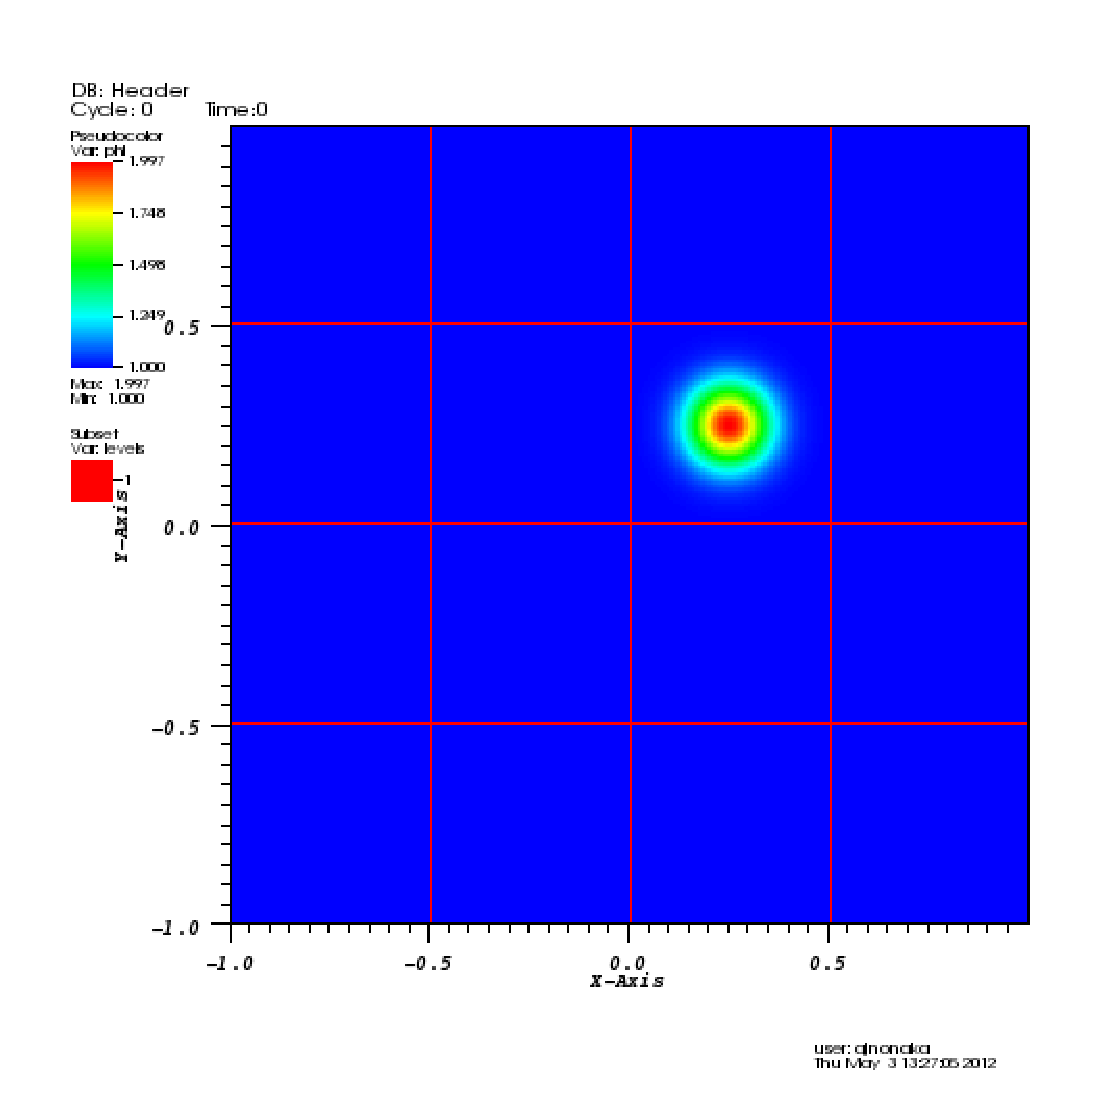
\includegraphics[width=3.1in]{./Visualization/VisIt_2D}
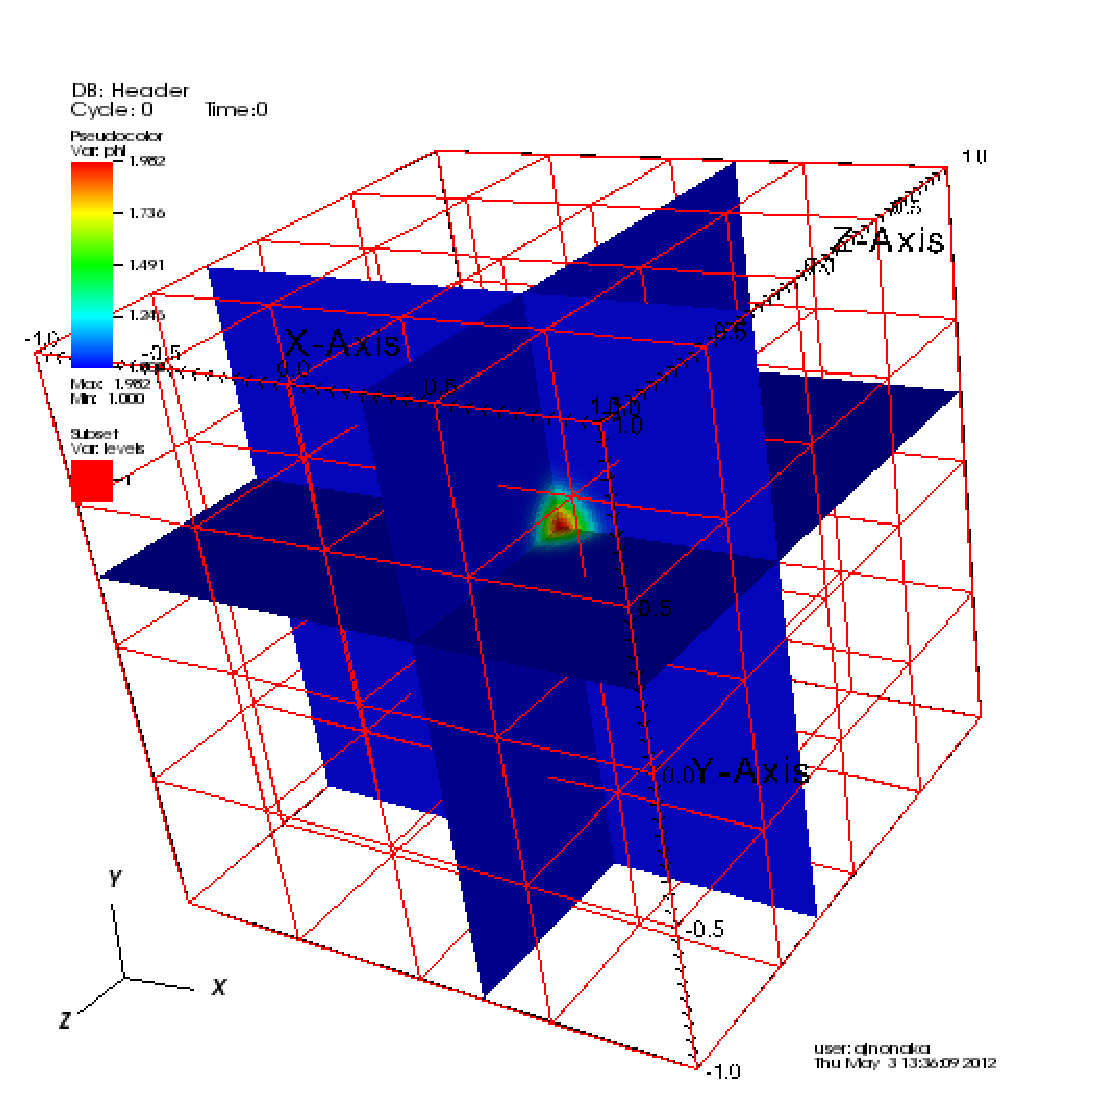
\includegraphics[width=3.1in]{./Visualization/VisIt_3D}
\caption{(Left) 2D image generated with VisIt.  (Right) 3D image generated with VisIt.}
\label{Fig:VisIt}
\end{figure}

In 3D, you must apply the ``Operators'' $\rightarrow$ ``Slicing'' $\rightarrow$ ``ThreeSlice'', with the 
``ThreeSlice operator attribute'' set to x=0.25, y=0.25, and z=0.25.  You can left-click and drag
over the image to rotate the image to generate something similar to right side of Figure \ref{Fig:VisIt}.\\

To make a movie, you must first create a text file named {\tt movie.visit} with a list of the {\tt Header} 
files for the individual frames.  This can most easily be done using the command:
\begin{lstlisting}[backgroundcolor=\color{light-red}]
~/amrex/Tutorials/Basic/HeatEquation_EX1_C> ls -1 plt*/Header | tee movie.visit
plt00000/Header
plt01000/Header
plt02000/Header
plt03000/Header
plt04000/Header
plt05000/Header
plt06000/Header
plt07000/Header
plt08000/Header
plt09000/Header
plt10000/Header
\end{lstlisting}
The next step is to run {\tt VisIt}, select ``File'' $\rightarrow$ ``Open file ...'',
then select {\tt movie.visit}.  Create an image to your liking and press the ``play'' button
on the VCR-like control panel to preview all the frames.  To save the movie, choose
``File'' $\rightarrow$ ``Save movie ...'', and follow the on-screen instructions.

\section{\paraview}
The open source visualization package \paraview\ v5.3.0 can be used to view 
3D plotfiles, and v5.4.0 can be used to view particle data.  Download
the package at \url{https://www.paraview.org/}.  

To open a single plotfile (for example, you could run the {\tt HeatEquation\_EX1\_C} in 3D:
\begin{enumerate}
\item Run \paraview\ v5.3.0, then select ``File'' $\rightarrow$ ``Open''.
\item Navigate to the plotfile directory, and manually type in ``Header''.
      \paraview\ will ask you about the file type -- choose ``Boxlib 3D Files''
\item Under the ``Cell Arrays'' field, select a variable (e.g., ``phi'') 
      and click ``Apply''.
\item Under ``Representation'' select ``Surface''.
\item Under ``Coloring'' select the variable you chose above.
\item To add planes, near the top left you will see a cube icon with a green plane
      slicing through it.  If you hover your mouse over it, it will say ``Slice''.
      Click that button.
\item You can play with the Plane Parameters to define a plane of data to view, as shown
      in Figure \ref{fig:ParaView}.
\end{enumerate}

\begin{figure}[tb]
\centering
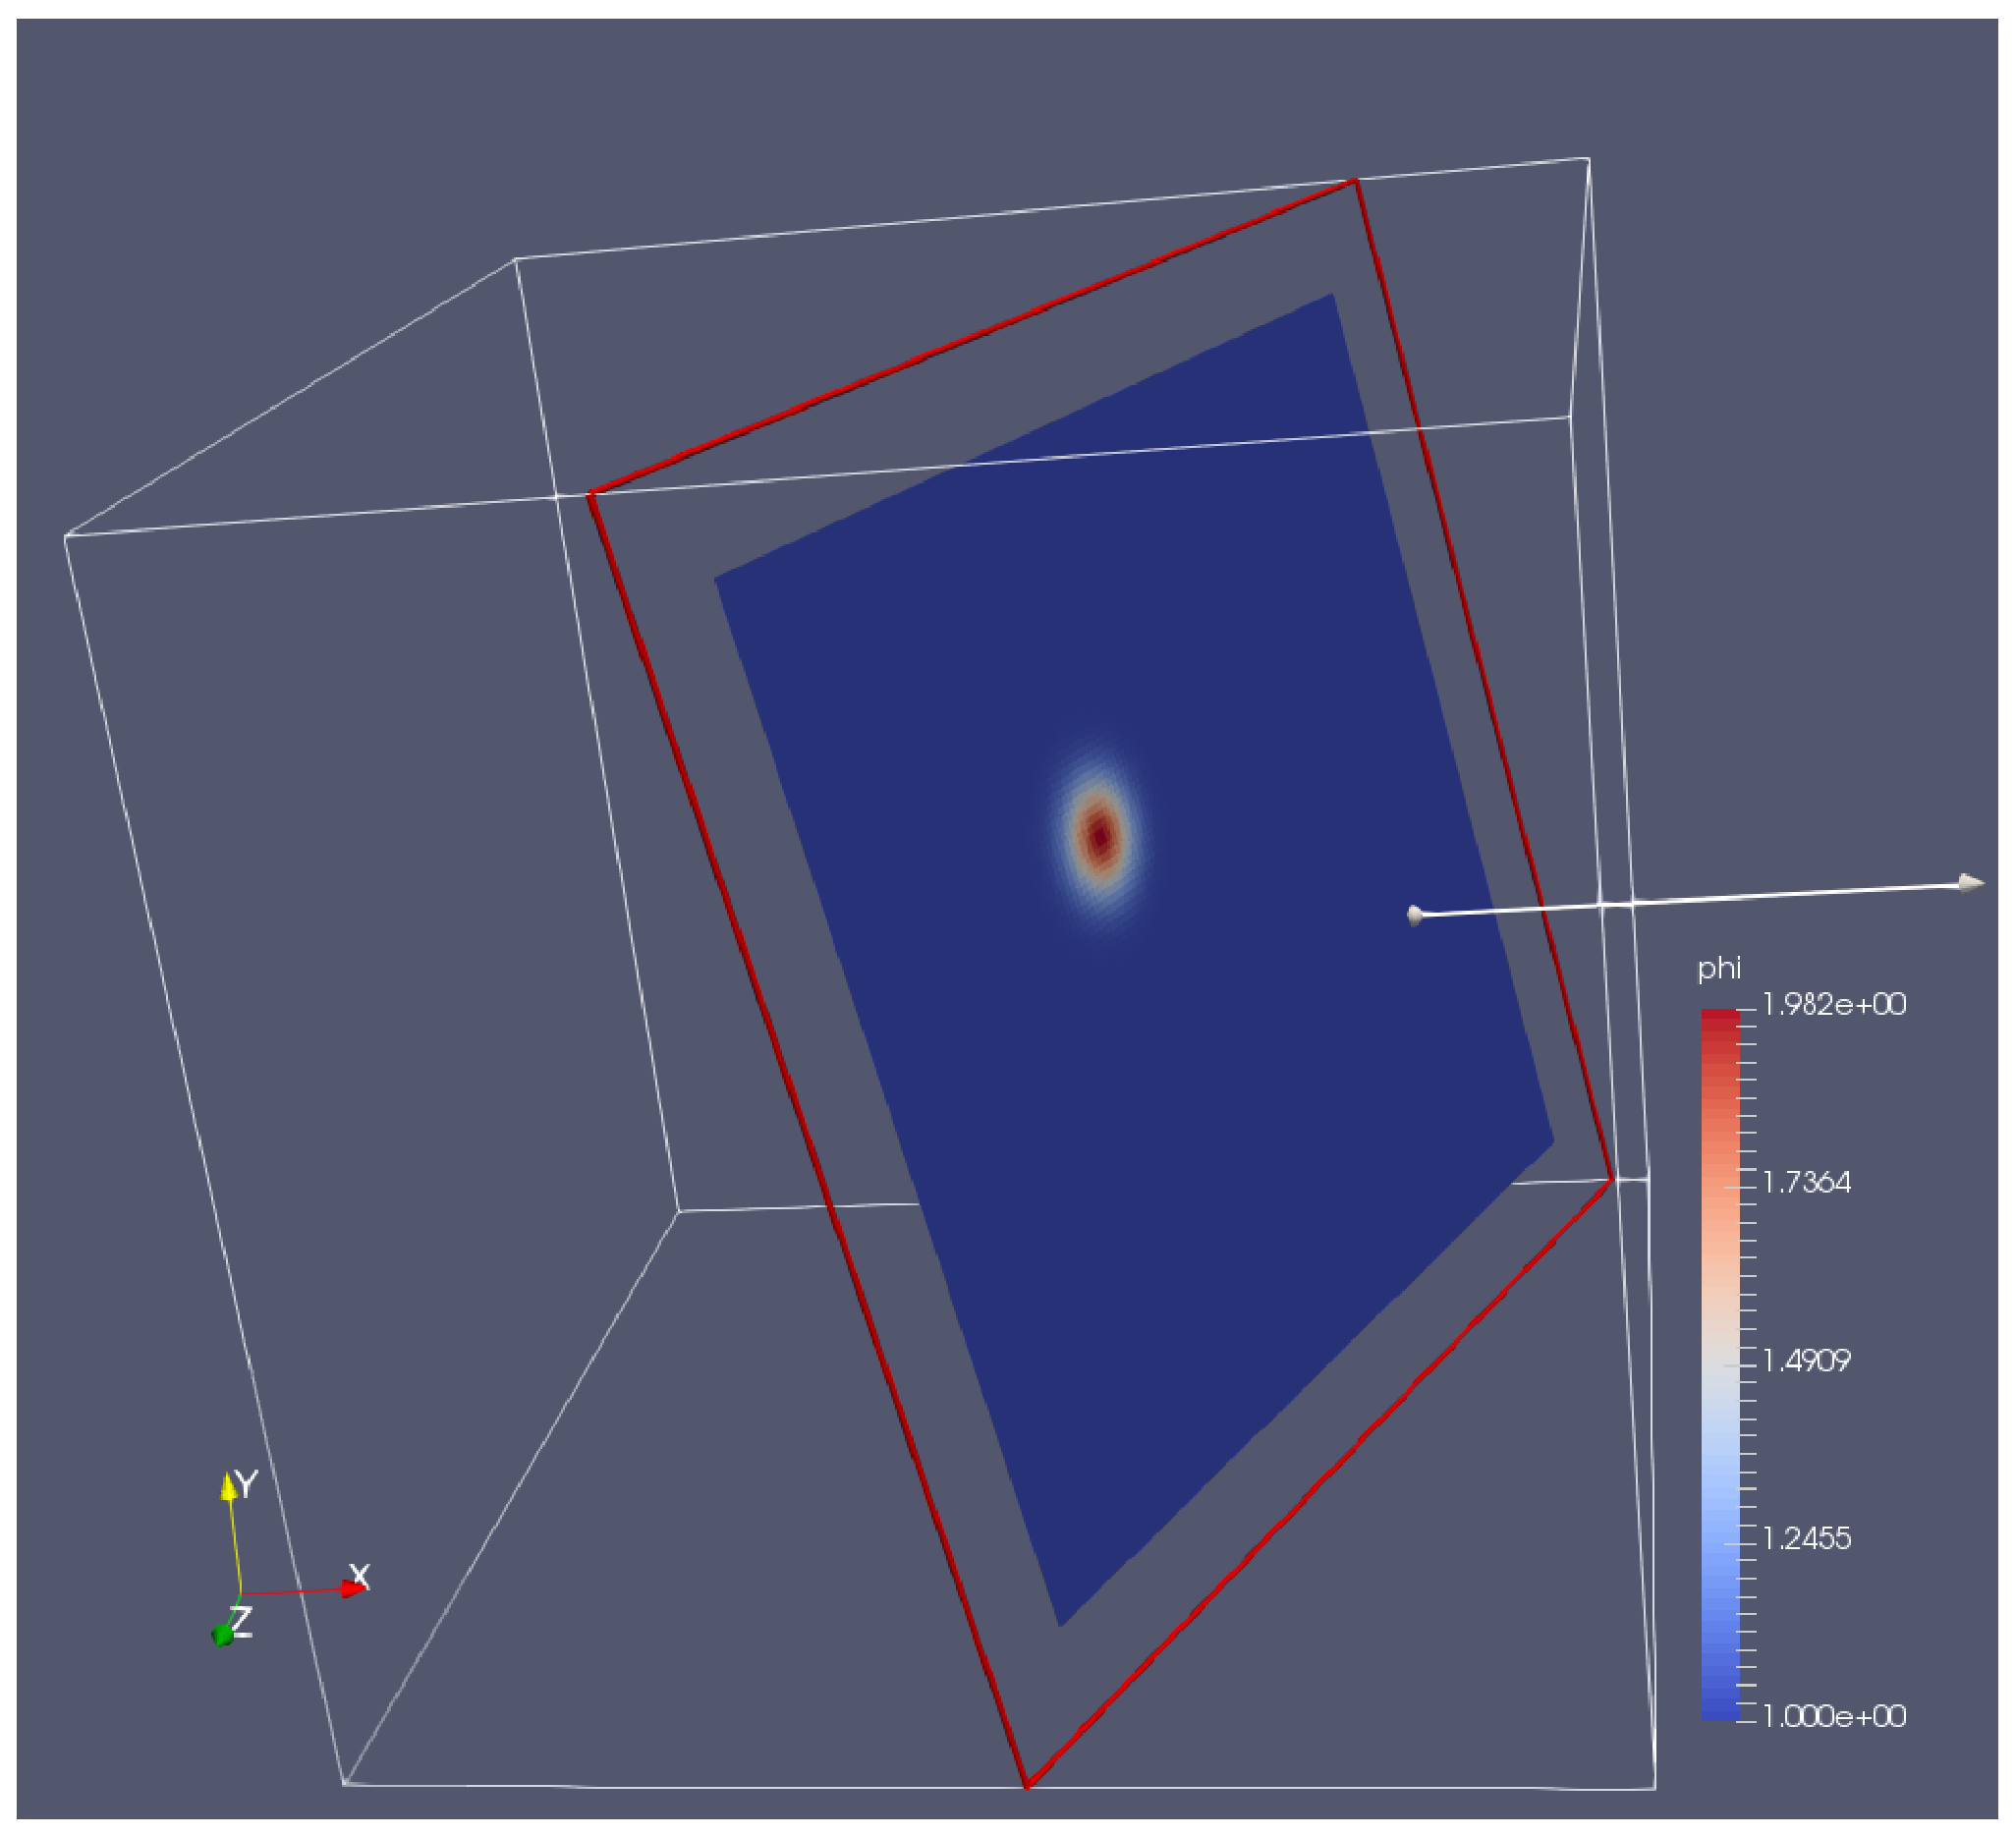
\includegraphics[width=3.1in]{./Visualization/ParaView}
\caption{Plotfile image generated with \paraview}
\label{fig:ParaView}
\end{figure}

To visualize particles (for example, you could run the {\tt ShortRangeParticles} example:
\begin{enumerate}
\item First, we have to convert the \amrex\ particle data to a format \paraview\ can read.
      In the run directory, there will be a sequence of particle files ({\tt particles00000},
      {\tt particles00001}, $\cdots$, {\tt particles01000}).
\item Run the script,
      {\tt amrex/Tools/Py\_util/amrex\_particles\_to\_vtp/amrex\_particles\_to\_vtp.py}
      as follows, e.g.,
      {\tt python amrex\_particles\_to\_vtp.py 0 1000 particles}.  You will generate
      a sequence of {\tt .vtp} files.
\item Run \paraview v5.4.0, and select ``File'' $\rightarrow$ ``Open''.  You will see
      a combined ``particles..vtp'' file grouping the files.  Select that and click OK.
\item Click ``Apply'' and under ``Representation'' select ``Point Gaussian''.
\item Change the Gaussian Radius if you like.  You can scroll through the frames with the
      VCR-like controls at the top, as shown in Figure \ref{fig:ParaView_particles}.
\end{enumerate}


\begin{figure}[tb]
\centering
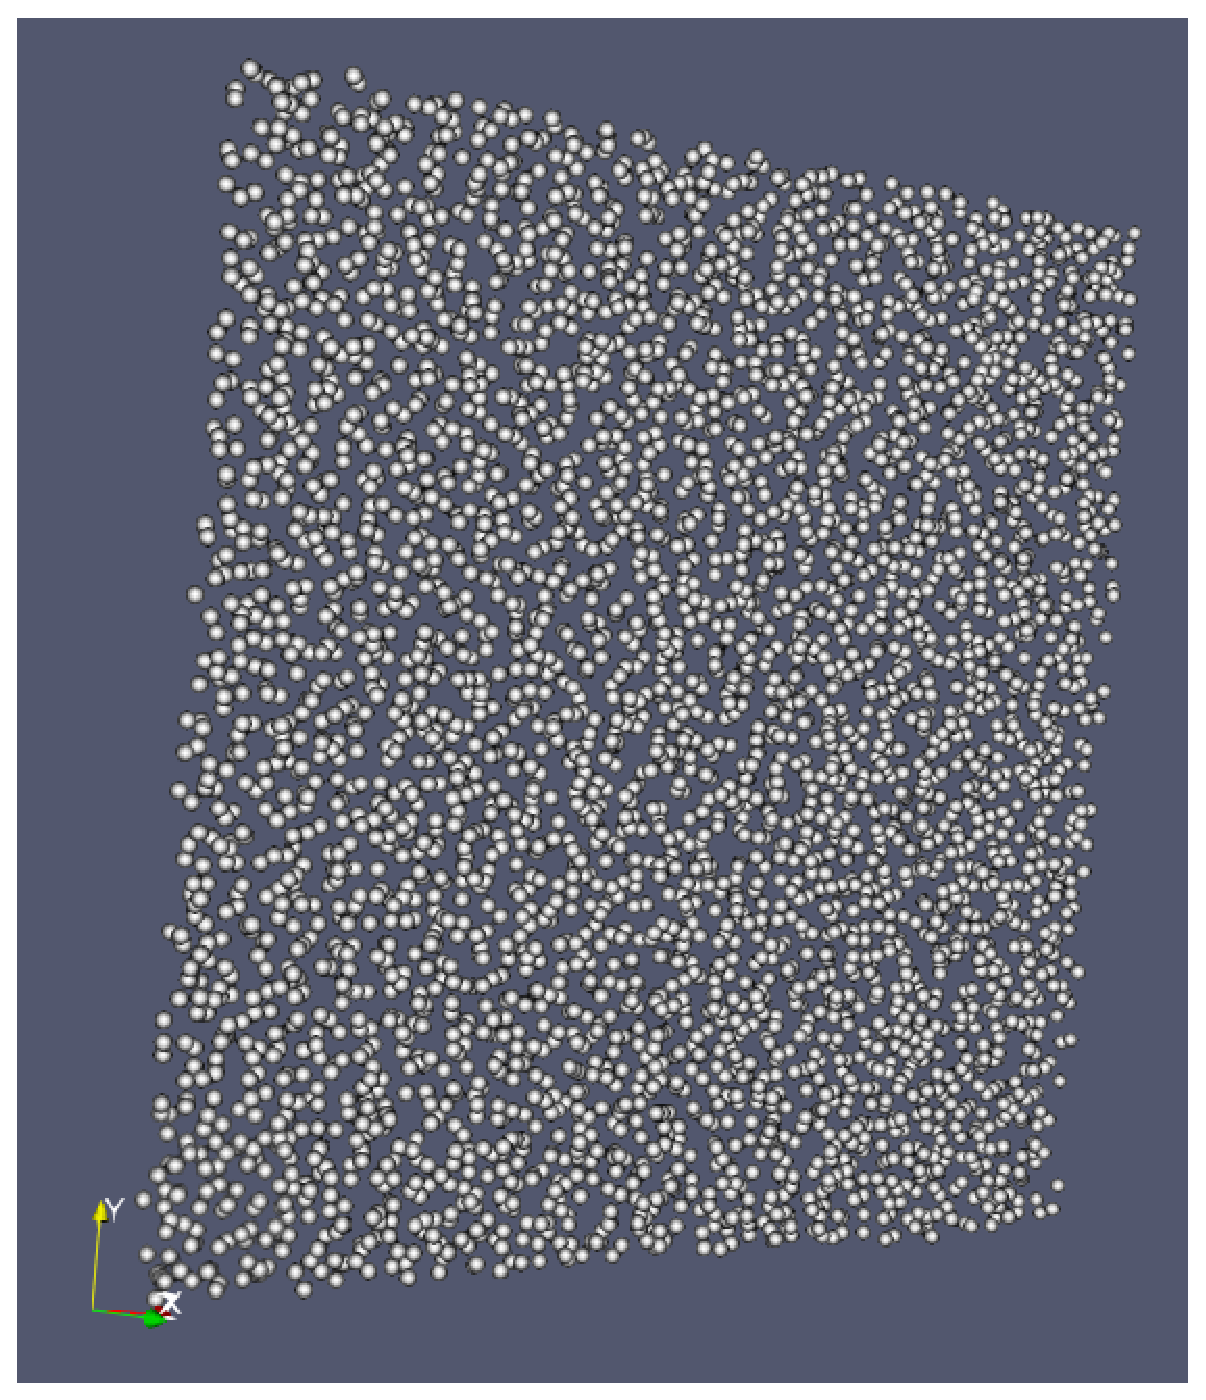
\includegraphics[width=3.1in]{./Visualization/ParaView_particles}
\caption{Particle image generated with \paraview}
\label{fig:ParaView_particles}
\end{figure}

\section{\yt}

\yt, an open source Python package available at \url{http://yt-project.org/},
can be used for analyzing and visualizing mesh and particle data generated by
\amrex\ codes.  Some of the \amrex\ developers are also \yt\ project members.
Below we describe how to use \yt\ on both a local workstation, as well as at
the NERSC HPC facility for high-throughput visualization of large data sets.

\subsection{Using \yt\ on a local workstation}

Running \yt\ on a local system generally provides good interactivity, but
limited performance. Consequently, this configuration is best when doing
exploratory visualization (e.g., experimenting with camera angles, lighting,
and color schemes) of small data sets.

To use \yt\ on an \amrex\ plot file, first start a Jupyter notebook or an IPython kernel, and import the \texttt{yt} module:

\begin{lstlisting}[language=python,breaklines=true]
In [1]: import yt

In [2]: print(yt.__version__)
3.4-dev
\end{lstlisting}

Next, load a plot file; in this example we use a plot file from the Nyx cosmology application:

\begin{lstlisting}[language=python,breaklines=true]
In [3]: ds = yt.load("plt00401")
yt : [INFO     ] 2017-05-23 10:03:56,182 Parameters: current_time              = 0.00605694344696544
yt : [INFO     ] 2017-05-23 10:03:56,182 Parameters: domain_dimensions         = [128 128 128]
yt : [INFO     ] 2017-05-23 10:03:56,182 Parameters: domain_left_edge          = [ 0.  0.  0.]
yt : [INFO     ] 2017-05-23 10:03:56,183 Parameters: domain_right_edge         = [ 14.24501  14.24501  14.24501]

In [4]: ds.field_list
Out[4]:
[('DM', 'particle_mass'),
 ('DM', 'particle_position_x'),
 ('DM', 'particle_position_y'),
 ('DM', 'particle_position_z'),
 ('DM', 'particle_velocity_x'),
 ('DM', 'particle_velocity_y'),
 ('DM', 'particle_velocity_z'),
 ('all', 'particle_mass'),
 ('all', 'particle_position_x'),
 ('all', 'particle_position_y'),
 ('all', 'particle_position_z'),
 ('all', 'particle_velocity_x'),
 ('all', 'particle_velocity_y'),
 ('all', 'particle_velocity_z'),
 ('boxlib', 'density'),
 ('boxlib', 'particle_mass_density')]
\end{lstlisting}

From here one can make slice plots, 3-D volume renderings, etc. An example of
the slice plot feature is shown below:

\begin{lstlisting}[language=python,breaklines=true]
In [9]: slc = yt.SlicePlot(ds, "z", "density")
yt : [INFO     ] 2017-05-23 10:08:25,358 xlim = 0.000000 14.245010
yt : [INFO     ] 2017-05-23 10:08:25,358 ylim = 0.000000 14.245010
yt : [INFO     ] 2017-05-23 10:08:25,359 xlim = 0.000000 14.245010
yt : [INFO     ] 2017-05-23 10:08:25,359 ylim = 0.000000 14.245010

In [10]: slc.show()

In [11]: slc.save()
yt : [INFO     ] 2017-05-23 10:08:34,021 Saving plot plt00401_Slice_z_density.png
Out[11]: ['plt00401_Slice_z_density.png']
\end{lstlisting}

The resulting image is Figure~\ref{fig:yt_Nyx_slice_plot}. One can also make
volume renderings with \yt; an example is show below:

\begin{figure}
  \includegraphics[scale=0.5]{./Visualization/yt_Nyx_density_slice.png}
  \caption{Slice plot of $128^3$ Nyx simulation using \yt.}
  \label{fig:yt_Nyx_slice_plot}
\end{figure}

\begin{lstlisting}[language=python,breaklines=true]
In [12]: sc = yt.create_scene(ds, field="density", lens_type="perspective")

In [13]: source = sc[0]

In [14]: source.tfh.set_bounds((1e8, 1e15))

In [15]: source.tfh.set_log(True)

In [16]: source.tfh.grey_opacity = True

In [17]: sc.show()
<Scene Object>:
Sources:
    source_00: <Volume Source>:YTRegion (plt00401): , center=[  1.09888770e+25   1.09888770e+25   1.09888770e+25] cm, left_edge=[ 0.  0.  0.] cm, right_edge=[  2.19777540e+25   2.19777540e+25   2.19777540e+25] cm transfer_function:None
Camera:
    <Camera Object>:
	position:[ 14.24501  14.24501  14.24501] code_length
	focus:[ 7.122505  7.122505  7.122505] code_length
	north_vector:[ 0.81649658 -0.40824829 -0.40824829]
	width:[ 21.367515  21.367515  21.367515] code_length
	light:None
	resolution:(512, 512)
Lens: <Lens Object>:
	lens_type:perspective
	viewpoint:[ 0.95423473  0.95423473  0.95423473] code_length

In [19]: sc.save()
yt : [INFO     ] 2017-05-23 10:15:07,825 Rendering scene (Can take a while).
yt : [INFO     ] 2017-05-23 10:15:07,825 Creating volume
yt : [INFO     ] 2017-05-23 10:15:07,996 Creating transfer function
yt : [INFO     ] 2017-05-23 10:15:07,997 Calculating data bounds. This may take a while.  Set the TranferFunctionHelper.bounds to avoid this.
yt : [INFO     ] 2017-05-23 10:15:16,471 Saving render plt00401_Render_density.png
\end{lstlisting}

The output of this is Figure~\ref{fig:yt_Nyx_vol_rend}.

\begin{figure}
  \includegraphics[scale=1.0]{./Visualization/yt_Nyx_density_vol_rend.png}
  \caption{Volume rendering of $128^3$ Nyx simulation using \yt. This
           corresponds to the same plot file used to generate the slice plot in
           Figure~\ref{fig:yt_Nyx_slice_plot}.}
  \label{fig:yt_Nyx_vol_rend}
\end{figure}

\subsection{Using \yt\ at NERSC (\emph{under development})}

Becase \yt\ is Python-based, it is portable and can be used in many software
environments. Here we focus on \yt's capabilities at NERSC, which provides
resources for performing both interactive and batch queue-based visualization
and analysis of \amrex\ data. Coupled with \yt's MPI and OpenMP parallelization
capabilities, this can enable high-throughput visualization and analysis
workflows.

\subsubsection{Interactive \yt\ with Jupyter notebooks}

Unlike \visit\ (\S\ref{sec:visit}), \yt\ has no client-server interface. Such
an interface is often crucial when one has large data sets generated on a
remote system, but wishes to visualize the data on a local workstation. Both
copying the data between the two systems, as well as visualizing the data
itself on a workstation, can be prohibitively slow.

Fortunately, NERSC has implemented several resources which allow one to
interact with \yt\ remotely, emulating a client-server model. In particular,
NERSC now hosts Jupyter notebooks which run IPython kernels on the Cori system;
this provides users access to the \texttt{\$HOME}, \texttt{/project}, and
\texttt{\$SCRATCH} file systems from a web browser-based Jupyter notebook.
\emph{\textbf{Please note that Jupyter hosting at NERSC is still under
development, and the environment may change without notice.}}

NERSC also provides Anaconda Python, which allows users to create their own
customizable Python environments. It is recommended to install \yt\ in such an
environment. One can do so with the following example:

\begin{lstlisting}
user@cori10:~> module load python/3.5-anaconda
user@cori10:~> conda create -p $HOME/yt-conda numpy
user@cori10:~> source activate $HOME/yt-conda
(/global/homes/u/user/yt-conda/) user@cori10:~> pip install yt
\end{lstlisting}

More information about Anaconda Python at NERSC is here:
\url{http://www.nersc.gov/users/data-analytics/data-analytics/python/anaconda-python/}.

One can then configure this Anaconda environment to run in a Jupyter notebook
hosted on the Cori system. Currently this is available in two places: on
\url{https://ipython.nersc.gov}, and on \url{https://jupyter-dev.nersc.gov}.
The latter likely reflects what the stable, production environment for Jupyter
notebooks will look like at NERSC, but it is still under development and
subject to change. To load this custom Python kernel in a Jupyter notebook,
follow the instructions at this URL under the ``Custom Kernels'' heading:
\url{http://www.nersc.gov/users/data-analytics/data-analytics/web-applications-for-data-analytics}.
After writing the appropriate \texttt{kernel.json} file, the custom kernel will
appear as an available Jupyter notebook. Then one can interactively visualize
\amrex\ plot files in the web browser.\footnote{It is convenient to use the
magic command \texttt{\%matplotlib inline} in order to render matplotlib
figures in the same browser window as the notebook, as opposed to displaying it
as a new window.}

\subsubsection{Parallel \yt}

Besides the benefit of no longer needing to move data back and forth between
NERSC and one's local workstation to do visualization and analysis, an
additional feature of \yt\ which takes advantage of the computational resources
at NERSC is its parallelization capabilities. \yt\ supports both MPI- and
OpenMP-based parallelization of various tasks, which are discussed here:
\url{http://yt-project.org/doc/analyzing/parallel_computation.html}.

Configuring \yt\ for MPI parallelization at NERSC is a more complex task than
discussed on the official \yt\ documentation; the command \texttt{pip install
mpi4py} is not sufficient. Rather, one must compile \texttt{mpi4py} from source
using the Cray compiler wrappers \texttt{cc}, \texttt{CC}, and \texttt{ftn} on
Cori. Instructions for compiling \texttt{mpi4py} at NERSC are provided here:
\url{http://www.nersc.gov/users/data-analytics/data-analytics/python/anaconda-python/#toc-anchor-3}.
After \texttt{mpi4py} has been compiled, one can use the regular Python
interpreter in the Anaconda environment as normal; when executing \yt\
operations which support MPI parallelization, the multiple MPI processes will
spawn automatically.

Although several components of \yt\ support MPI parallelization, a few are particularly useful:
\begin{itemize}
  \item \textbf{Time series analysis.} Often one runs a simulation for many
time steps and periodically writes plot files to disk for visualization and
post-processing. \yt\ supports parallelization over time series data via the
\texttt{DatasetSeries} object. \yt\ can iterate over a \texttt{DatasetSeries}
in parallel, with different MPI processes operating on different elements of
the series. This page provides more documentation:
\url{http://yt-project.org/doc/analyzing/time_series_analysis.html#time-series-analysis}.

  \item \textbf{Volume rendering}. \yt\ implements spatial decomposition among
MPI processes for volume rendering procedures, which can be computationally
expensive. Note that \yt\ also implements OpenMP parallelization in volume
rendering, and so one can execute volume rendering with a hybrid MPI+OpenMP
approach. See this URL for more details:
\url{http://yt-project.org/doc/visualizing/volume_rendering.html?highlight=openmp#openmp-parallelization}.

  \item \textbf{Generic parallelization over multiple objects.} Sometimes one
wishes to loop over a series which is not a \texttt{DatasetSeries}, e.g.,
performing translational or rotational operations on a camera to make a volume
rendering in which the field of view moves through the simulation. In this
case, one is applying a set of operations on a single object (a single plot
file), rather than over a time series of data. For this workflow, \yt\ provides
the \texttt{parallel\_objects()} function. See this URL for more details:
\url{http://yt-project.org/doc/analyzing/parallel_computation.html#parallelizing-over-multiple-objects}.

An example of MPI parallelization in \yt\ is shown below, where one animates a
time series of plot files from an IAMR simulation while revolving the camera
such that it completes two full revolutions over the span of the animation:

\begin{lstlisting}[language=python,breaklines=true]
import yt
import glob
import numpy as np

yt.enable_parallelism()

base_dir1 = '/global/cscratch1/sd/user/Nyx_run_p1'
base_dir2 = '/global/cscratch1/sd/user/Nyx_run_p2'
base_dir3 = '/global/cscratch1/sd/user/Nyx_run_p3'

glob1 = glob.glob(base_dir1 + '/plt*')
glob2 = glob.glob(base_dir2 + '/plt*')
glob3 = glob.glob(base_dir3 + '/plt*')

files = sorted(glob1 + glob2 + glob3)

ts = yt.DatasetSeries(files, parallel=True)

frame = 0
num_frames = len(ts)
num_revol = 2

slices = np.arange(len(ts))

for i in yt.parallel_objects(slices):
    sc = yt.create_scene(ts[i], lens_type='perspective', field='z_velocity')

    source = sc[0]
    source.tfh.set_bounds((1e-2, 9e+0))
    source.tfh.set_log(False)
    source.tfh.grey_opacity = False

    cam = sc.camera

    cam.rotate(num_revol*(2.0*np.pi)*(i/num_frames),
               rot_center=np.array([0.0, 0.0, 0.0]))

    sc.save(sigma_clip=5.0)
\end{lstlisting}

When executed on 4 CPUs on a Haswell node of Cori, the output looks like the following:

\begin{lstlisting}[breaklines=true]
user@nid00009:~/yt_vis/> srun -n 4 -c 2 --cpu_bind=cores python make_yt_movie.py
yt : [INFO     ] 2017-05-23 16:51:33,565 Global parallel computation enabled: 0 / 4
yt : [INFO     ] 2017-05-23 16:51:33,565 Global parallel computation enabled: 2 / 4
yt : [INFO     ] 2017-05-23 16:51:33,566 Global parallel computation enabled: 1 / 4
yt : [INFO     ] 2017-05-23 16:51:33,566 Global parallel computation enabled: 3 / 4
P003 yt : [INFO     ] 2017-05-23 16:51:33,957 Parameters: current_time              = 0.103169376949795
P003 yt : [INFO     ] 2017-05-23 16:51:33,957 Parameters: domain_dimensions         = [128 128 128]
P003 yt : [INFO     ] 2017-05-23 16:51:33,957 Parameters: domain_left_edge          = [ 0.  0.  0.]
P003 yt : [INFO     ] 2017-05-23 16:51:33,958 Parameters: domain_right_edge         = [ 6.28318531  6.28318531  6.28318531]
P000 yt : [INFO     ] 2017-05-23 16:51:33,969 Parameters: current_time              = 0.0
P000 yt : [INFO     ] 2017-05-23 16:51:33,969 Parameters: domain_dimensions         = [128 128 128]
P002 yt : [INFO     ] 2017-05-23 16:51:33,969 Parameters: current_time              = 0.0687808060674485
P000 yt : [INFO     ] 2017-05-23 16:51:33,969 Parameters: domain_left_edge          = [ 0.  0.  0.]
P002 yt : [INFO     ] 2017-05-23 16:51:33,969 Parameters: domain_dimensions         = [128 128 128]
P000 yt : [INFO     ] 2017-05-23 16:51:33,970 Parameters: domain_right_edge         = [ 6.28318531  6.28318531  6.28318531]
P002 yt : [INFO     ] 2017-05-23 16:51:33,970 Parameters: domain_left_edge          = [ 0.  0.  0.]
P002 yt : [INFO     ] 2017-05-23 16:51:33,970 Parameters: domain_right_edge         = [ 6.28318531  6.28318531  6.28318531]
P001 yt : [INFO     ] 2017-05-23 16:51:33,973 Parameters: current_time              = 0.0343922351851018
P001 yt : [INFO     ] 2017-05-23 16:51:33,973 Parameters: domain_dimensions         = [128 128 128]
P001 yt : [INFO     ] 2017-05-23 16:51:33,974 Parameters: domain_left_edge          = [ 0.  0.  0.]
P001 yt : [INFO     ] 2017-05-23 16:51:33,974 Parameters: domain_right_edge         = [ 6.28318531  6.28318531  6.28318531]
P000 yt : [INFO     ] 2017-05-23 16:51:34,589 Rendering scene (Can take a while).
P000 yt : [INFO     ] 2017-05-23 16:51:34,590 Creating volume
P003 yt : [INFO     ] 2017-05-23 16:51:34,592 Rendering scene (Can take a while).
P002 yt : [INFO     ] 2017-05-23 16:51:34,592 Rendering scene (Can take a while).
P003 yt : [INFO     ] 2017-05-23 16:51:34,593 Creating volume
P002 yt : [INFO     ] 2017-05-23 16:51:34,593 Creating volume
P001 yt : [INFO     ] 2017-05-23 16:51:34,606 Rendering scene (Can take a while).
P001 yt : [INFO     ] 2017-05-23 16:51:34,607 Creating volume
\end{lstlisting}

Because the \texttt{parallel\_objects()} function transforms the loop into a
data-parallel problem, this procedure strong scales nearly perfectly to an
arbitrarily large number of MPI processes, allowing for rapid rendering of
large time series of data.

\end{itemize}


\chapter{Profiling}\label{Chap:Profiling}
\amrex-based application codes can be instrumented using AMReX-specific performance
profiling tools that take into account the hierarchical nature of the mesh in 
most AMReX-based applications.  These codes can be instrumented for varying levels of 
profiling detail.  The broad-brush C++ instrumentation is as follows:

\section{Instrumenting the Code} 
\subsection{C++} 

\begin{lstlisting}[language=cpp]
void YourClass::YourFunction() 
{
  BL_PROFILE("YourClass::YourFunction()");  // this name can be any string

  // your function code
}
\end{lstlisting}

For other timers within an already instrumented function, add:
 
\begin{lstlisting}[language=cpp]
      BL_PROFILE_VAR("Flaten::FORT_FLATENX()", anyname);  // add this before
        FORT_FLATENX(arg1, arg2);
      BL_PROFILE_VAR_STOP(anyname);   // add this after, using the same name
\end{lstlisting}
 
if you want to use the same name within the same scope, you can use:
 
\begin{lstlisting}[language=cpp]
      BL_PROFILE_VAR("MyFuncs()", myfuncs);  // the first one
        MyFunc_0(arg);
      BL_PROFILE_VAR_STOP(myfuncs);
      ...
      BL_PROFILE_VAR_START(myfuncs);
        MyFunc_1(arg);
      BL_PROFILE_VAR_STOP(myfuncs);
\end{lstlisting}
 
or create a profiling variable without starting, then start/stop:
 
\begin{lstlisting}[language=cpp]
      BL_PROFILE_VAR_NS("MyFuncs()", myfuncs);  // dont start the timer
      ...
      BL_PROFILE_VAR_START(myfuncs);
        MyFunc_0(arg);
      BL_PROFILE_VAR_STOP(myfuncs);
      ...
      BL_PROFILE_VAR_START(myfuncs);
        MyFunc_1(arg);
      BL_PROFILE_VAR_STOP(myfuncs);
\end{lstlisting}

\subsection{Fortran90} 

Fortran90 functions can also be instrumented with the following calls:
 
\begin{lstlisting}[language=fortran]
call bl_proffortfuncstart("my_function")
...
call bl_proffortfuncstop("my_function")
\end{lstlisting}
 
Note that the start and stop calls must be matched and the profiling output will warn of any 
{\tt bl\_proffortfuncstart} calls that were not stopped with {\tt bl\_proffortfuncstop} calls
(in debug mode only).  You will need to add {\tt bl\_proffortfuncstop}
before any returns and at the end of the function or at the point in the
function you want to stop profiling. 

\section{Types of Profiling} 

Currently you have two options for AMReX-specific profiling.  If you set {\tt TINY\_PROFILE = TRUE}
in your GNUMakefile then at the end of the run, a summary of exclusive and inclusive function times 
will be written to stdout.

If you set {\tt PROFILE = TRUE} then a {\tt bl\_prof} directory will be written that contains 
detailed per-task timings of the code.    An exclusive-only set of function timings will be written to stdout

If, in addition to  {\tt PROFILE = TRUE}, you set {\tt TRACE\_PROFILE = TRUE}, then the profiler keeps track
of when each profiled function is called and  the {\tt bl\_prof} directory will include the function call stack.   
This is especially useful when core functions, such as {\tt FillBoundary} can be called from many different regions of the code.
Part of the trace profiling is the ability to set regions in the code which can be analyzed for profiling information independently from other regions. 

If, in addition to  {\tt PROFILE = TRUE}, you set {\tt COMM\_PROFILE = TRUE}, then the {\tt bl\_prof} directory 
will contain additional information about MPI communication (point-to-point timings, data volume, barrier/reduction times, etc.).  {\tt TRACE\_PROFILE = TRUE} and {\tt COMM\_PROFILE = TRUE} can be set together.

The AMReX-specific profiling tools are currently under development and this documentation will reflect the latest 
status in the development branch.

\section{Sample Output}

Sample output from {\tt TINY\_PROFILE = TRUE} can look like the following:


\begin{lstlisting}[basicstyle=\tiny,tabsize=1]

TinyProfiler total time across processes [min...avg...max]: 1.765...1.765...1.765
---------------------------------------------------------------------------------
Name                          NCalls   Excl. Min   Excl. Avg   Excl. Max   Max  %
---------------------------------------------------------------------------------
mfix_level::EvolveFluid       1        1.602       1.668       1.691       95.83%
FabArray::FillBoundary()      11081    0.02195     0.03336     0.06617      3.75%
FabArrayBase::getFB()         22162    0.02031     0.02147     0.02275      1.29%
PC<...>::WriteAsciiFile()     1        0.00292     0.004072    0.004551     0.26%


---------------------------------------------------------------------------------
Name                          NCalls   Incl. Min   Incl. Avg  Incl. Max    Max  %
---------------------------------------------------------------------------------
mfix_level::Evolve()          1        1.69        1.723      1.734        98.23%
mfix_level::EvolveFluid       1        1.69        1.723      1.734        98.23%
FabArray::FillBoundary()      11081    0.04236     0.05485    0.08826       5.00%
FabArrayBase::getFB()         22162    0.02031     0.02149    0.02275       1.29%

\end{lstlisting}

\section{\tt AMRProfParser} 

{\tt AMRProfParser} is a tool for processing and analyzing the {\tt bl\_prof} database.  It is a
command line application that can create performance summaries, plotfiles showing
point to point communication and timelines, HTML call trees, communication call
statistics, function timing graphs, and other data products.  The parser's data
services functionality can be called from an interactive environment such as {\tt Amrvis},
from a sidecar for dynamic performance optimization, and from other utilities such as
the command line version of the parser itself.  It has been integrated into {\tt Amrvis}
for visual interpretation of the data allowing {\tt Amrvis} to open the {\tt bl\_prof} database
like a plotfile but with interfaces appropriate to profiling data. AMRProfParser
and {\tt Amrvis} can be run in parallel both interactively and in batch mode.



%\chapter{Debugging}\label{Chap:Debugging}
%Debugging is an art and everyone has their own preferred method.  In
this chapter, we will present a few techniques that might be useful
for \amrex\ users.

\section{Debug Build, Floating-Point Exceptions and Backtrace}
\label{sec:debug:fpe}

There are a lot of assertions in \amrex.  These assertions are turned
off for optimized build.  When debugging, we find it is helpful to
build with debug options.  For example, for building with GNU Make
(Chapter~\ref{Chap:BuildingAMReX}), one can type {\tt make DEBUG=TRUE}
to turn on debug options.  In addition to assertions, this will also
add various compiler options such as floating pointer exception
trapping, fortran array bound checking, etc.  For floating pointer
exception trapping, one should use {\tt ParmParse} parameter {\tt
amrex.fpe\_trap\_invalid=1}.  (Note that one can append this option to
the command line without modifying the inputs file.)  This parameter
can be used to initialize all {\tt MultiFab} data to signaling NaNs.
If an assertion fails or a floating point exception occurs, backtrace
files named {\tt Backtrace.*} will be generated, one for each parallel
process.  We can then examine the contents of these backtrace files
and hopefully they can tell us where in the code the problem occurs.

% send a signal

% Compile with Backtrace = True

% section on tools like valgrind, git bisect

% section on vismf diffmf fcompare




\chapter{CVODE}\label{Chap:CVODE}
\amrex\ supports local ODE integration using the \cvode\ solver,\footnote{\url{https://computation.llnl.gov/projects/sundials/cvode}} which is part of the \sundials\ framework.\footnote{\url{https://computation.llnl.gov/projects/sundials}}
\cvode\ contains solvers for stiff and non-stiff ODEs, and as such is well suited for solving e.g., the complex chemistry networks in combustion simulations, or the nuclear reaction networks in astrophysical simulations.

Most of \cvode\ is written in C, but many functions also come with two distinct Fortran interfaces.
One interface is \fcvode, which is bundled with the stable release of \cvode.
Its usage is described in the \cvode\ documentation.\footnote{\url{https://computation.llnl.gov/sites/default/files/public/cv_guide.pdf}}
However, the use of \fcvode\ is discouraged in \amrex\ due to its incompatibility with being used inside OpenMP parallel regions (which is the primary use case in \amrex\ applications).

The alternative, and recommended, Fortran interface to \cvode\ uses the \texttt{iso\_c\_binding} feature of the Fortran 2003 standard to implement a direct interface to the C functions in \cvode.
When compiling \cvode, one need not build the \cvode\ library with the \fcvode\ interface enabled at all.
Rather, the Fortran 2003 interface to \cvode\ is provided within \amrex\ itself.
The \cvode\ tutorials provided in \amrex\ use this new interface.

\section{Compiling \cvode}

To use \cvode\ in an \amrex\ application, follow these steps:

\begin{enumerate}

  \item Obtain the \cvode\ source code, which is hosted here: \url{https://computation.llnl.gov/projects/sundials/sundials-software}.

  One can download either the complete \sundials\ package, or just the \cvode\ components.

  \item Unpack the \cvode/\sundials\ tarball, and create a new ``build'' directory (it can be anywhere).

  \item Navigate to the new, empty build directory, and type

  \begin{verbatim}
  cmake \
    -DCMAKE_INSTALL_PREFIX:PATH=/path/to/install/dir \
    /path/to/cvode/or/sundials/top/level/source/dir
  \end{verbatim}

  The \texttt{CMAKE\_INSTALL\_DIR} option tells CMake where to install the libraries.
  Note that CMake will attempt to deduce the compilers automatically, but respects certain environment variables if they are defined, such as \texttt{CC} (for the C compiler), \texttt{CXX} (for the C++ compiler), and \texttt{FC} (for the Fortran compiler).
  So one may modify the above CMake invocation to be something like the following:

  \begin{verbatim}
  CC=/path/to/gcc \
  CXX=/path/to/g++ \
  FC=/path/to/gfortran \
    cmake \
    -DCMAKE_INSTALL_PREFIX:PATH=/path/to/install/dir \
    /path/to/cvode/or/sundials/top/level/source/dir
  \end{verbatim}

  One can supply additional flags to CMake or to the compiler to customize the compilation process. 
  Flags of interest may include \texttt{CMAKE\_C\_FLAGS}, which add the specified flags to the compile statement, e.g.,
  \texttt{-DCMAKE\_C\_FLAGS="-h list=a"} will append the \texttt{-h list=a} flag to the \texttt{cc} statement when compiling the source code.
  Here one may wish to add something like \texttt{"-O2 -g"} to provide an optimized library that still contains debugging symbols; 
  if one neglects debugging symbols in the \cvode\ library, and if a code that uses \cvode\ encounters a segmentation fault in the solve, 
  then the backtrace has no information about where in the solver the error occurred.
  Also, if one wishes to compile only the solver library itself and not the examples that come with the source 
  (compiling the examples is enabled by default), one can add \texttt{"-DEXAMPLES\_ENABLE=OFF"}.

  \item In the \texttt{GNUmakefile} for the \amrex\ application which uses the Fortran 2003 interface to \cvode, add \texttt{USE\_CVODE = TRUE}, which will compile the Fortran 2003 interfaces and link the \cvode\ libraries.
  Note that one must define the \texttt{CVODE\_LIB\_DIR} environment variable to point to the location where the libraries are installed.
\end{enumerate}


\section{The \cvode\ Tutorials}

\amrex\ provides two \cvode\ tutorials in the \texttt{Tutorials/CVODE} directory, called \texttt{EX1} and \texttt{EX2}.
\texttt{EX1} consists of a single ODE that is integrated with \cvode\ within each cell of a 3-D grid.
It demonstrates how to initialize the \cvode\ solver, how to call the ODE right-hand-side (RHS), and, more importantly, how to \emph{re-}initialize the solver between cells, which avoids allocating and freeing solver memory between each cell (see the call to \texttt{FCVReInit()} in the \texttt{integrate\_ode.f90} file in the \texttt{EX1} directory.)

The \texttt{EX2} example demonstrates the slightly more complicated case of integrating a system of coupled ODEs within each cell.
Similarly to \texttt{EX1}, it provides an RHS and some solver initialization.
However, it also demonstrates the performance effect of providing an analytic Jacobian matrix for the system of ODEs, 
rather than requiring the \cvode\ solver to compute the Jacobian matrix numerically using a finite-difference approach.
The tutorial integrates the same system of ODEs on the same 3-D grid, but in one sweep it instructs \cvode\ 
to use the analytic function that computes the Jacobian matrix, and in the other case, it does not,
which requires \cvode\ to compute it manually.
One observes a significant performance gain by providing the analytic Jacobian function.


%------------------------------------------------------------------------------
\backmatter

% \renewcommand\bibname{References}
% \addcontentsline{toc}{chapter}{References}
% \bibliographystyle{plain}
% \bibliography{refs,Verification/verification,Gravity/gr}

%\cleardoublepage
%\phantomsection
%\addcontentsline{toc}{chapter}{Index}
%\printindex

\end{document}
